\chapter{Implementación hardware del robot}
\label{cap:capitulo5}

\begin{flushright}
\begin{minipage}[]{10cm}
\emph{La perfección se logra no cuando no hay nada más que añadir, sino cuando no hay nada más que quitar}\\
\end{minipage}\\

Antoine de Saint-Exupéry\\
\end{flushright}

\vspace{1cm}

Tras haber expuesto todas las plataformas de desarrollo utilizadas en este proyecto, en este capítulo se describirá el proceso paso a paso, desde la concepción inicial hasta la construcción y ensamblaje, para que sea completamente operativo el robot.

\section{Geometría del robot}

En este apartado se detalla el proceso llevado a cabo para definir la idea y la forma elegida para el robot.

La aplicación de este proyecto se encuentra dentro de los robots de campo y es por ello que estos tipos de robots son mayoritariamente plataformas que trabajan en entornos no estructurados, como se comentó en el Capítulo 1. Por ello, es necesario que la estructura del robot se asemeje a esos tipos de robots y los más comunes son los robots con ruedas. 

Sin embargo los robots de campo son de gran coste y de grandes dimensiones, lo que hacía inviable que entidades con recursos limitados pudieran adquirirlos. Es por ello que se decidió apostar por los robots de bajo coste y gracias a Julio Vega y a su Pibot se pudo encontrar una primera idea hasta conseguir la solución final al proyecto. 

El artículo \cite{vega18c} presenta PiBot (Figura \ref{fig:pibot}), una plataforma robótica educativa  de 20x10x8 cm basada en Raspberry Pi 3 y PiCamera, diseñada para facilitar la enseñanza de robótica a estudiantes de secundaria. Ofrece una infraestructura de \textit{software} abierta en Python y comandos de alto nivel para facilitar el aprendizaje. Además, incluye un modelo 3D imprimible y una versión simulada en Gazebo, disponibles públicamente para que estudiantes y escuelas puedan aprender y practicar robótica sin necesidad del robot físico. 

\begin{figure} [h!]
	\begin{center}
		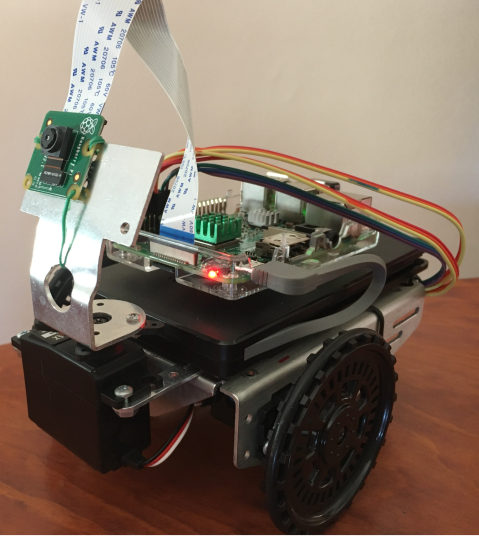
\includegraphics[width=6cm]{figs/cap5/Original.png}
	\end{center}
	\caption{Pibot} 
	\label{fig:pibot}
\end{figure}

Para poder continuar con la investigación de este proyecto, se creó una estructura de metal para que la cámara cambiase su disposición, mirase hacia el suelo y estuviese del derecho para evitar futuros cálculos innecesarios. El diseño hasta ese momento quedó como muestra la Figura \ref{fig:pibotmetal}.


\begin{figure} [h!]
	\begin{center}
		\includegraphics[width=8cm]{figs/cap5/new.png}
	\end{center}
	\caption{Pibot con cámara modificada} 
	\label{fig:pibotmetal}
\end{figure}


De este robot interesa que tiene dos grados de libertad para el movimiento del robot, ya que cuenta con dos ruedas con motores independientes y una rueda loca, lo que le permite desplazarse a lo largo del eje X como girar sobre sí misma. Otro grado de libertad que ha resultado útil para la aplicación de este proyecto es el giro sobre el eje Z del motor sobre el que está montada la cámara y poder aumentar el campo de visión. Así lo muestra la Figura \ref{fig:esquemaDOF}, señalados en rojo.


\begin{figure} [h!]
	\begin{center}
		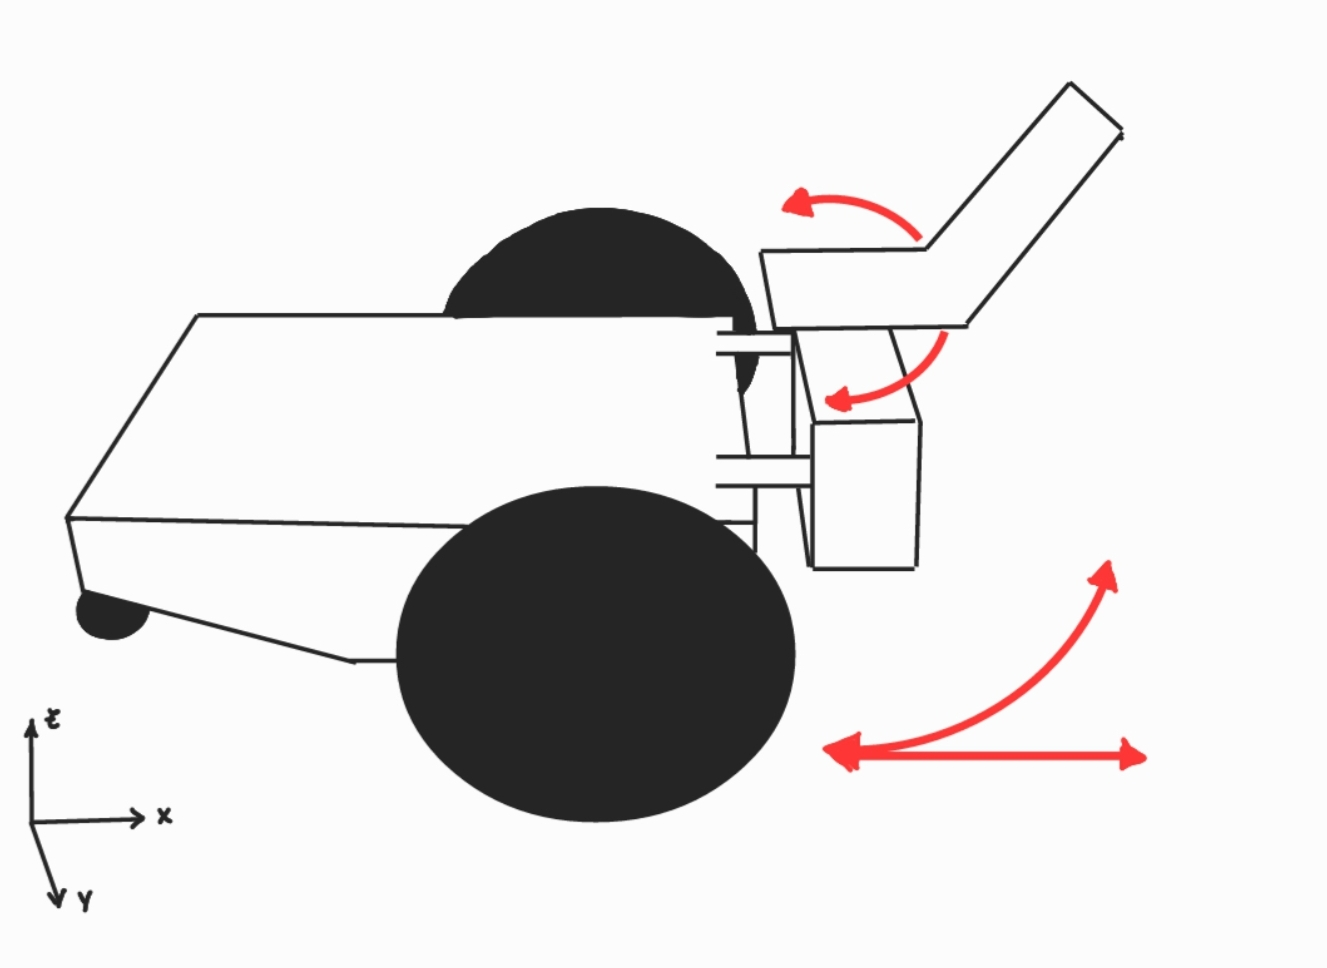
\includegraphics[width=9cm]{figs/cap5/dof.jpg}
	\end{center}
	\caption{Esquema de los grados de libertad de Pibot} 
	\label{fig:esquemaDOF}
\end{figure}


Para poder cumplir con el objetivo principal descrito en el Capítulo 3, es necesario añadir una serie de componentes \textit{hardware} para poder formar el esqueleto completo del robot.

\section{Elección de componentes hardware}

Una vez definida la geometría del robot, bautizado como Pibotj, es necesario elegir los componentes que más se ajustan para poder confeccionar el esqueleto del robot. Para ellos se ha creado un esquema (Figura \ref{fig:fritzzing}) que muestra todos los componentes necesarios y sus conexiones. A continuación, se van a explicar cada uno de los componentes \textit{hardware} elegidos.  

\begin{figure} [h!]
	\begin{center}
		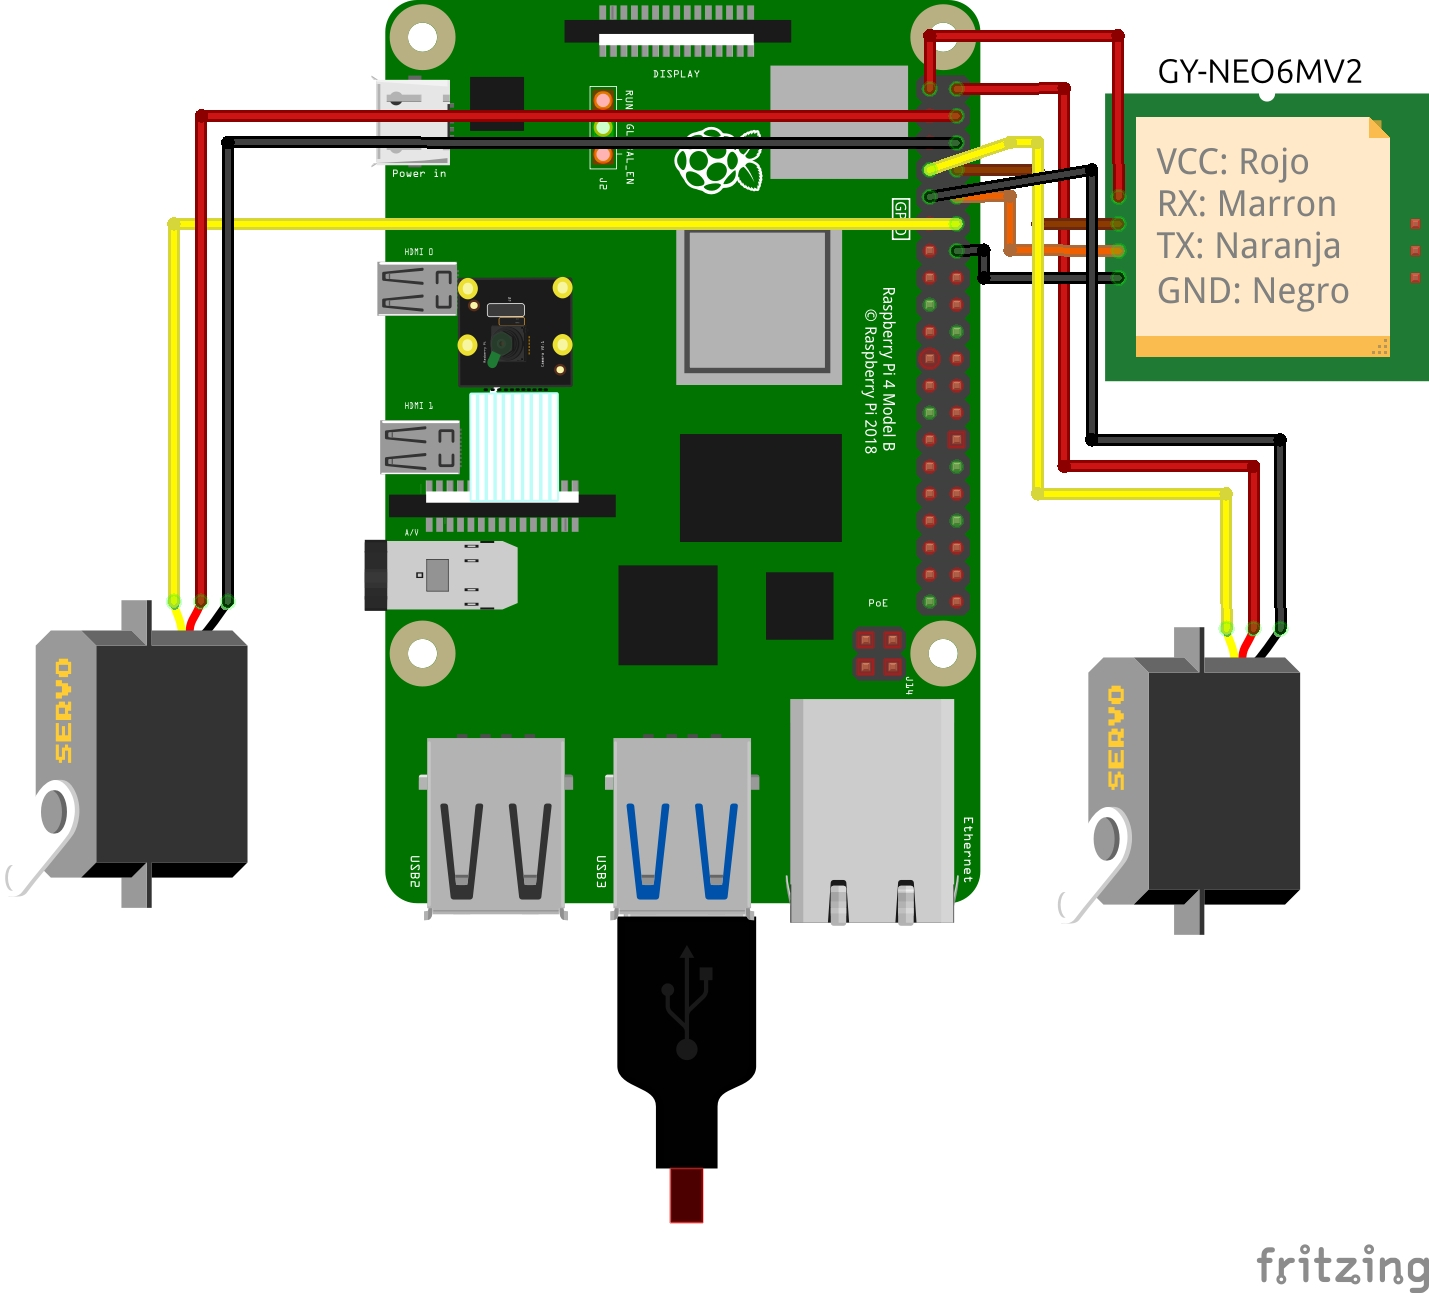
\includegraphics[width=9cm]{figs/cap5/modelocompleto_bb.jpg}
	\end{center}
	\caption{Esquema de conexiones del Pibotj} 
	\label{fig:fritzzing}
\end{figure}


\subsection{Raspberry Pi 4}

Es muy usado en robótica, ordenador a bordo,....



\subsection{Servomotores Parallax}
La fuerza, la utilidad que hacen,...


\subsection{Ruedas ActivityBot}
La fuerza, la utilidad que hacen,...

\subsection{Rueda Loca}
La fuerza, la utilidad que hacen,...

\subsection{Raspberry Pi Cámara}

Calidad de la imagen, parámetros intrínsecos teóricos,... 

\subsection{GPS NEO 6M}
Explicar el módulo GPS .... pruebas, alcance... tarda en coger señal, la luz azul...

\subsection{Google Coral USB}

Utilidades, el nivel de cómputo que llega,... inferencias por segundo,tipo de modelos compatible...

\subsection{Powerbank}
 
 Todo el día encendida y ejecutando, aguanta perfectamente... \\
 
  
  
 Distribuir los componentes (foto de fritzing): motores, sensores, cámaras (fotos mías)
 
 
 Explicar todos los componentes usados: 
 
 Si se incluyen imágenes que sean distintas a las del apartado de plataformas de desarrollo o no incluirlas. 
 
 Fotos hechas por mí 
 
 Uso las características que he aprovechado del capítulo 4 
 
 
\section{Bocetos}

La realización de bocetos es una etapa fundamental en el proceso de diseño que se realiza antes de iniciar el modelado en 3D, ya que su propósito es obtener una visión clara de la estructura y disposición de los componentes que conforman el Pibotj. Una vez que se ha definido el esqueleto completo que este necesitará, es el momento de crear una serie de bocetos (Figura \ref{fig:bocetos}) que permitirán afinar los detalles antes de realizar el diseño en 3D.

\begin{figure}[ht!]
	\centering
	\begin{minipage}{0.4\linewidth}
		\centering
		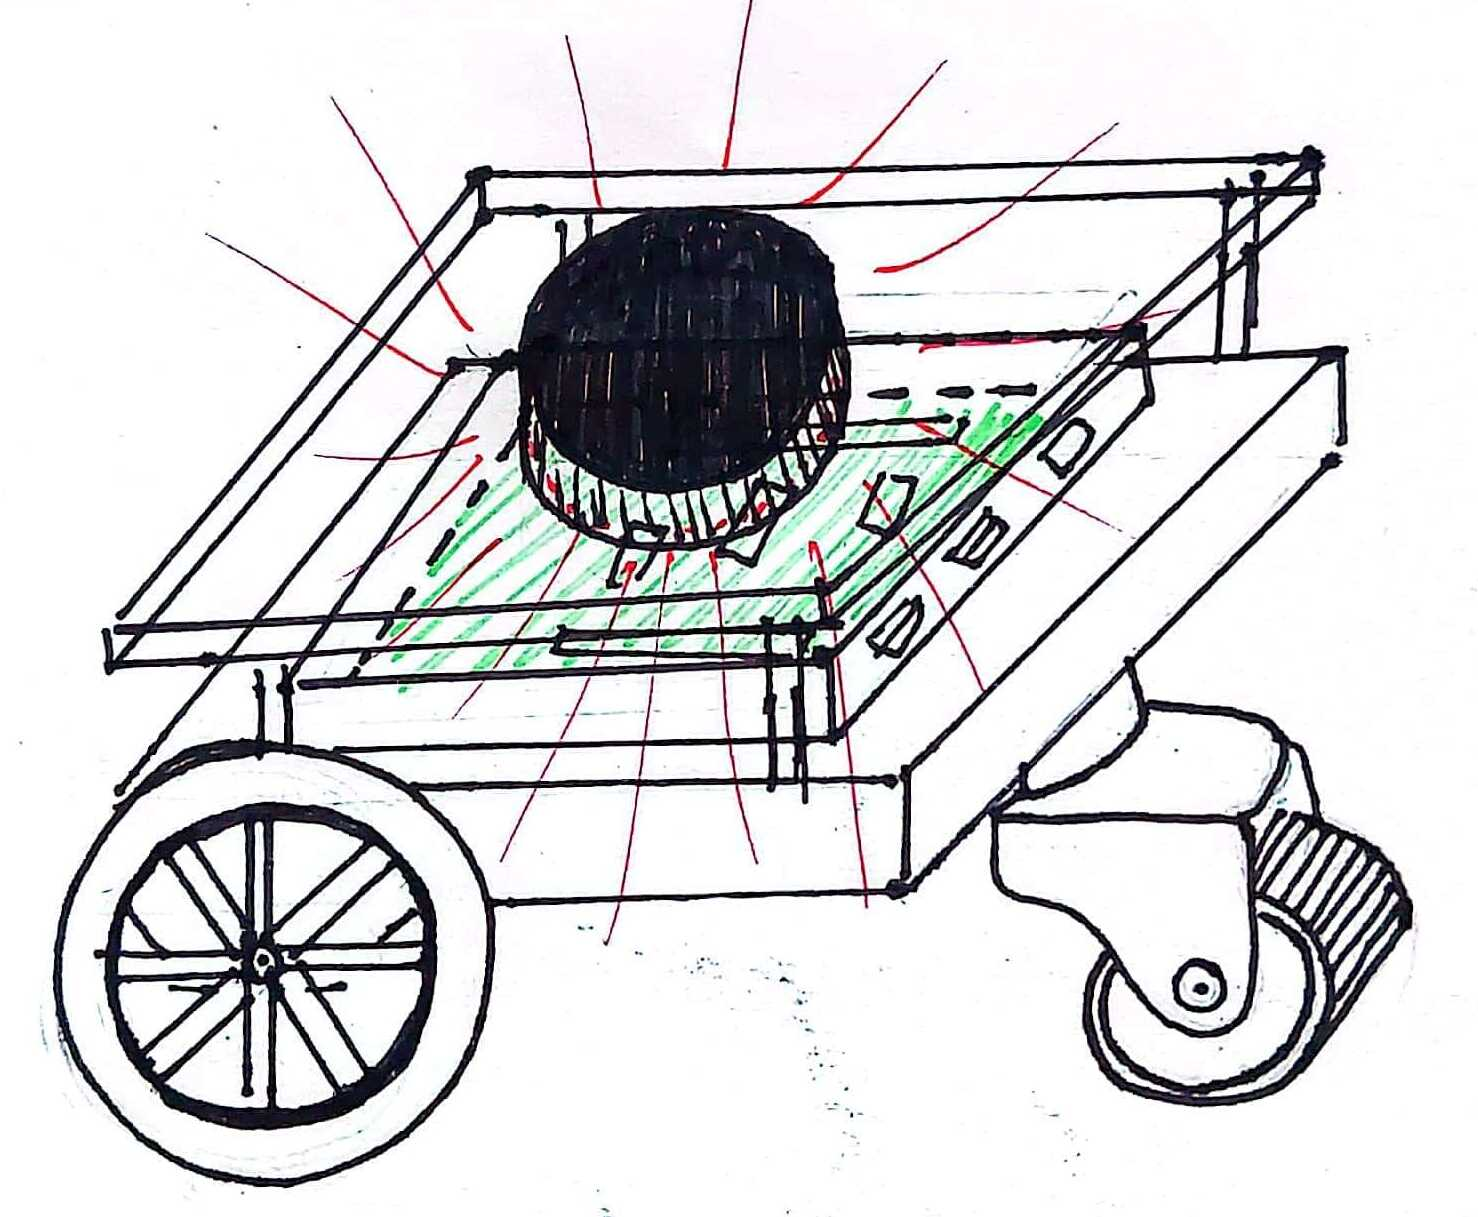
\includegraphics[width=\linewidth]{figs/cap5/prototipo_laser.jpeg}
	\end{minipage}
	\hspace{2cm}
	\begin{minipage}{0.4\linewidth}
		\centering
		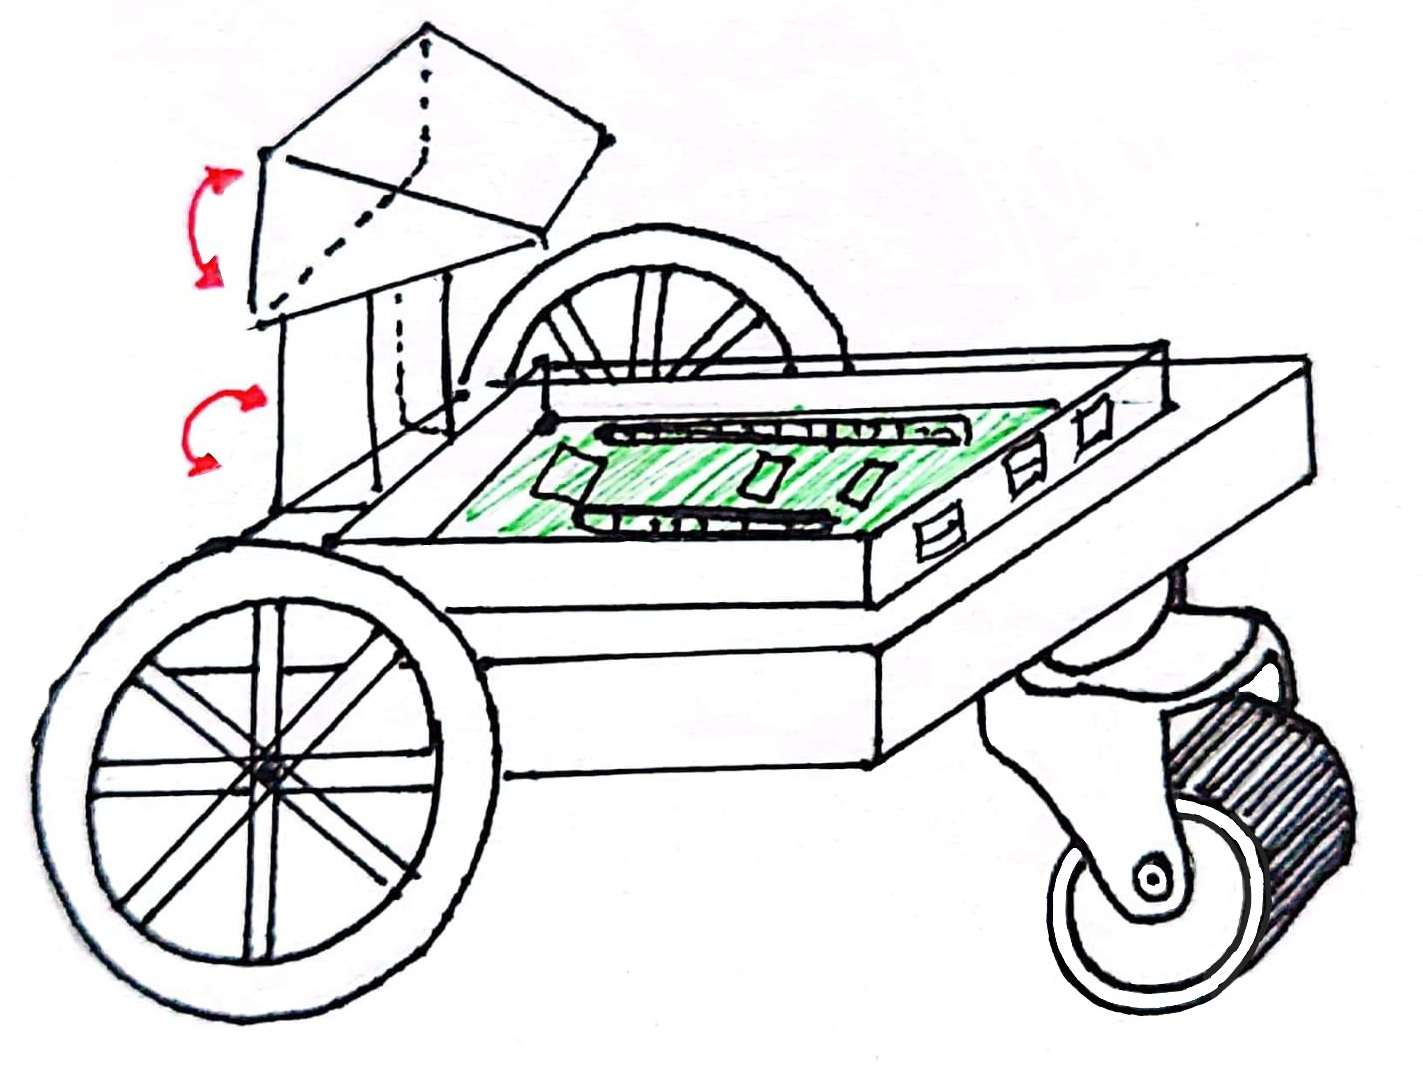
\includegraphics[width=\linewidth]{figs/cap5/prototipo_sin_laser.jpeg}
	\end{minipage}
	\hspace{2cm}
	\begin{minipage}{0.5\linewidth}
		\centering
		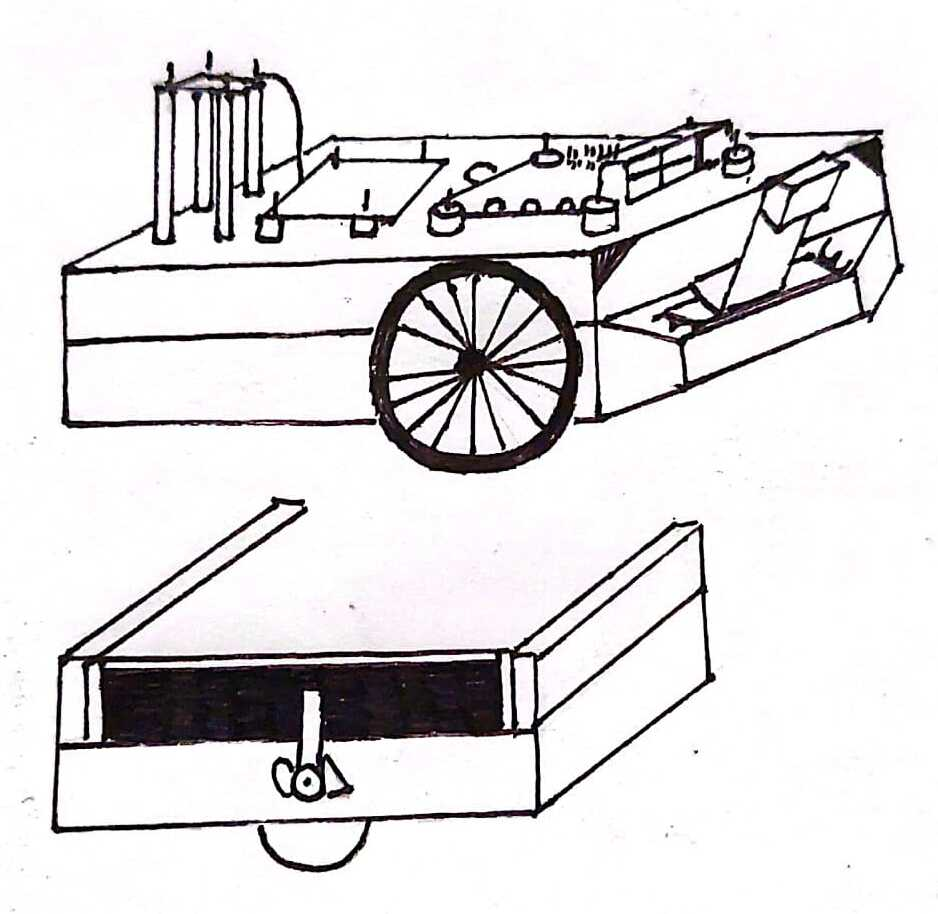
\includegraphics[width=\linewidth]{figs/cap5/boceto_papel.jpeg}
	\end{minipage}
	\caption{Bocetos creados a mano}
	\label{fig:bocetos}
\end{figure}

Antes de realizar el diseño \acs{CAD} de las piezas, se creó una maqueta a tamaño real (Figuras \ref{fig:maqueta1} y \ref{fig:maqueta2}) para poder tener una idea de cómo sería la aplicación final y así intentar no malgastar material de impresión. 

\begin{figure}[ht!]
	\centering
	\begin{minipage}{0.5\linewidth}
		\centering
		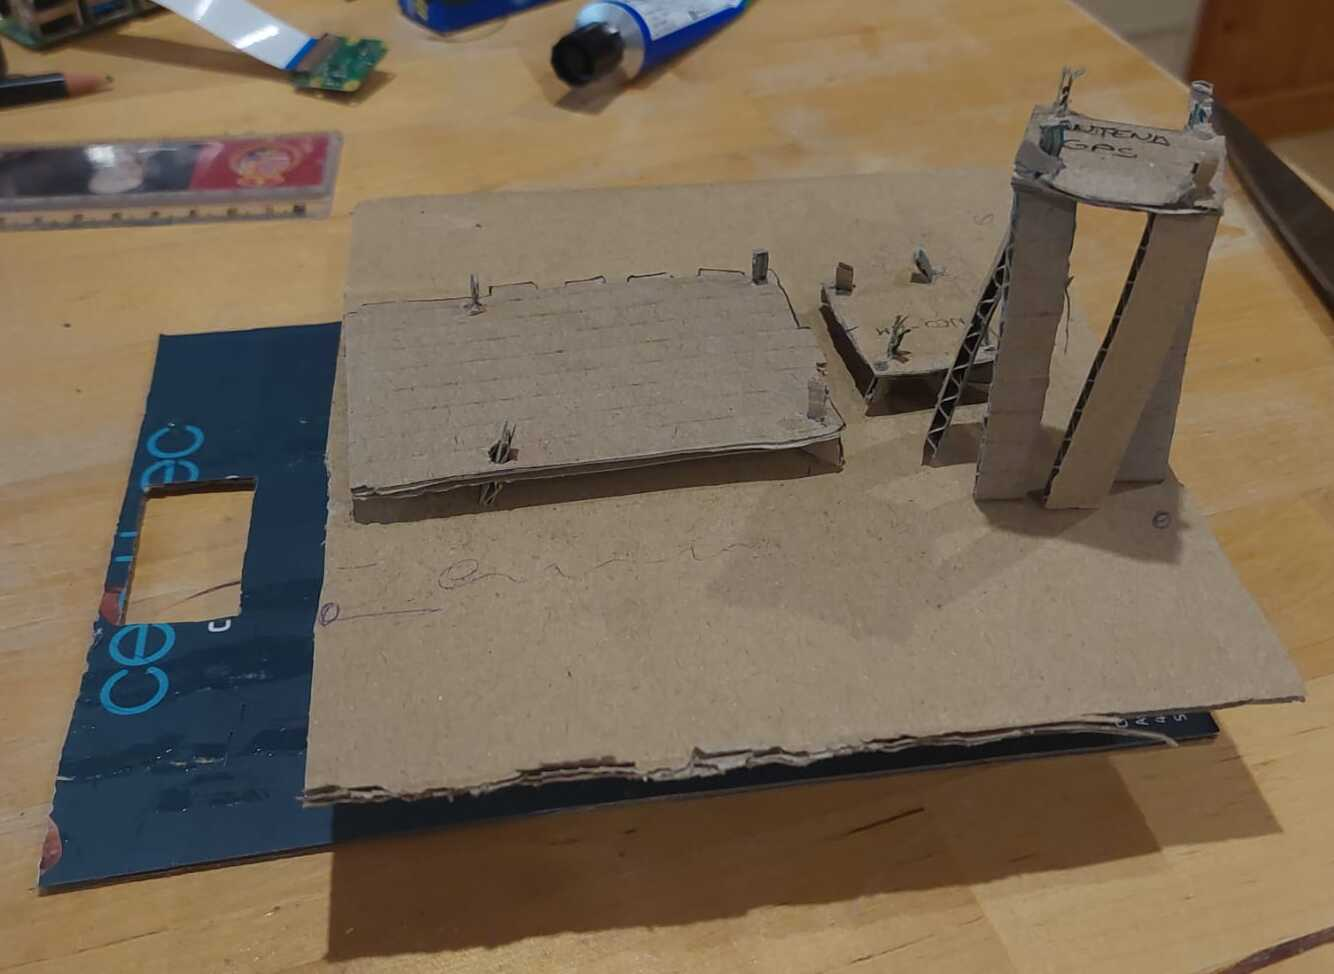
\includegraphics[width=\linewidth]{figs/cap5/boceto_carton1.jpeg}
		\caption*{\centering}
	\end{minipage}
	\hspace{1cm}
	\begin{minipage}{0.4\linewidth}
		\centering
		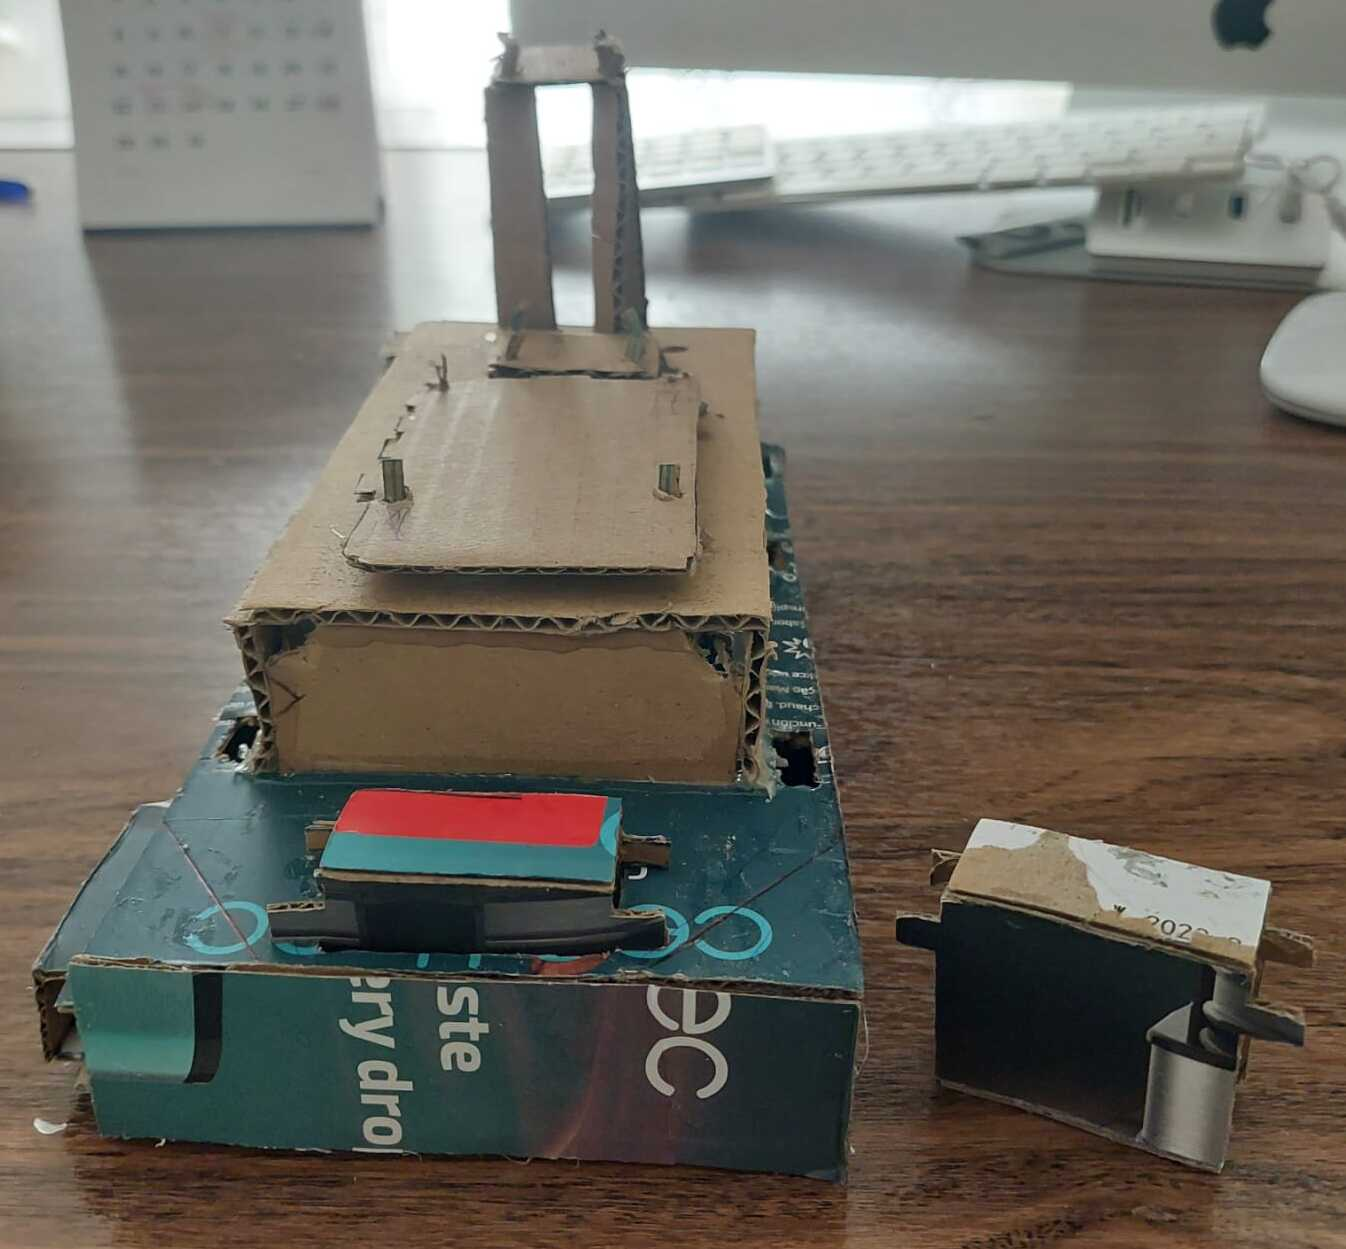
\includegraphics[width=\linewidth]{figs/cap5/boceto_carton2.jpeg}
		\caption*{\centering}
	\end{minipage}
	\hspace{2cm}
	\begin{minipage}{0.4\linewidth}
		\centering
		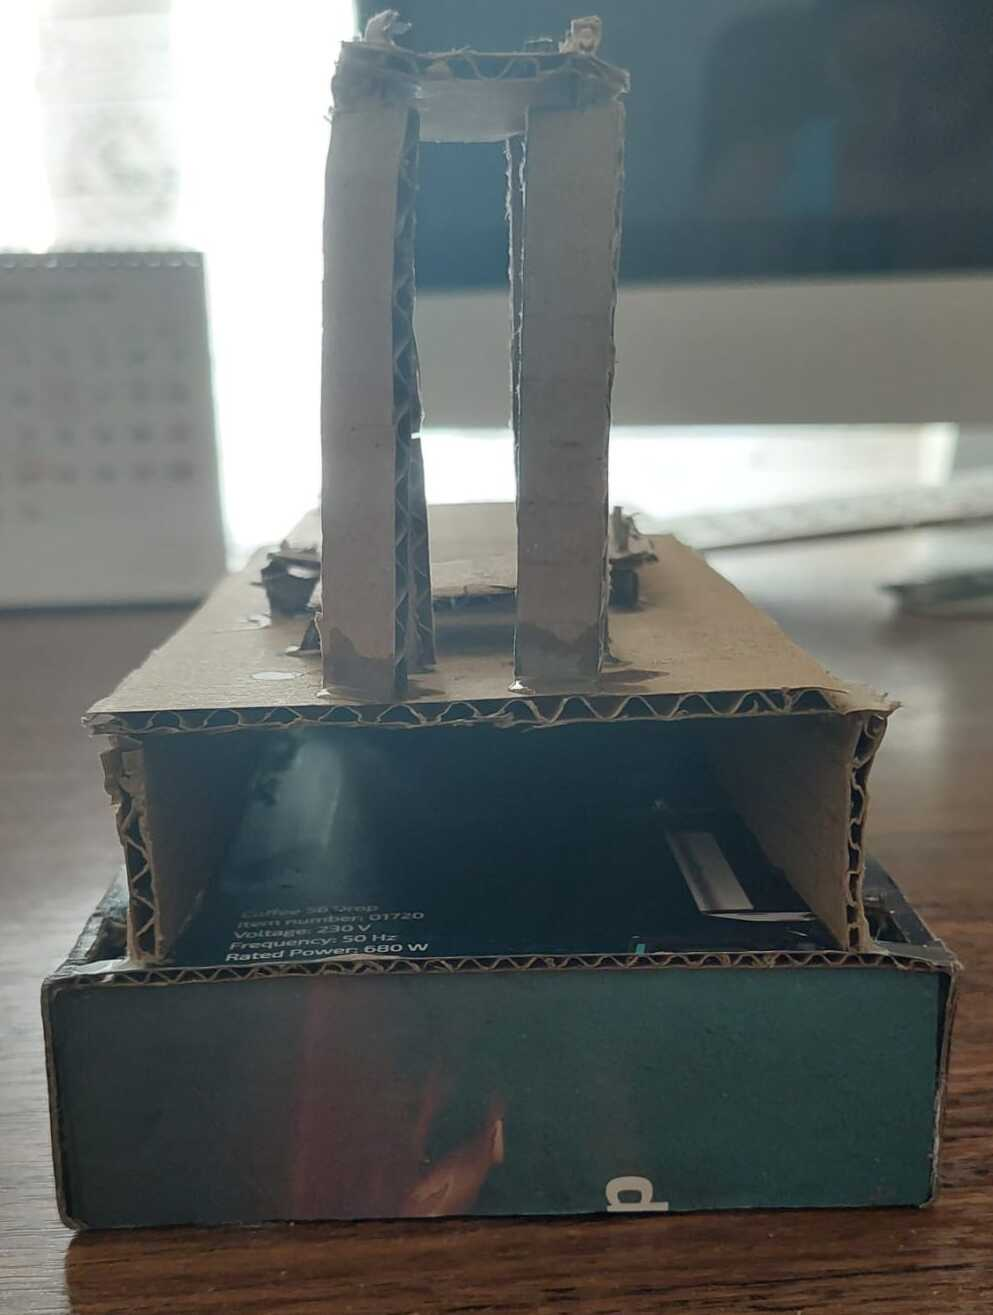
\includegraphics[width=\linewidth]{figs/cap5/boceto_carton3.jpeg}
		\caption*{\centering}
	\end{minipage}
	\caption{Maqueta en proceso}
	\label{fig:maqueta1}
\end{figure}

\begin{figure}[ht!]
	\centering
	\begin{minipage}{0.44\linewidth}
		\centering
		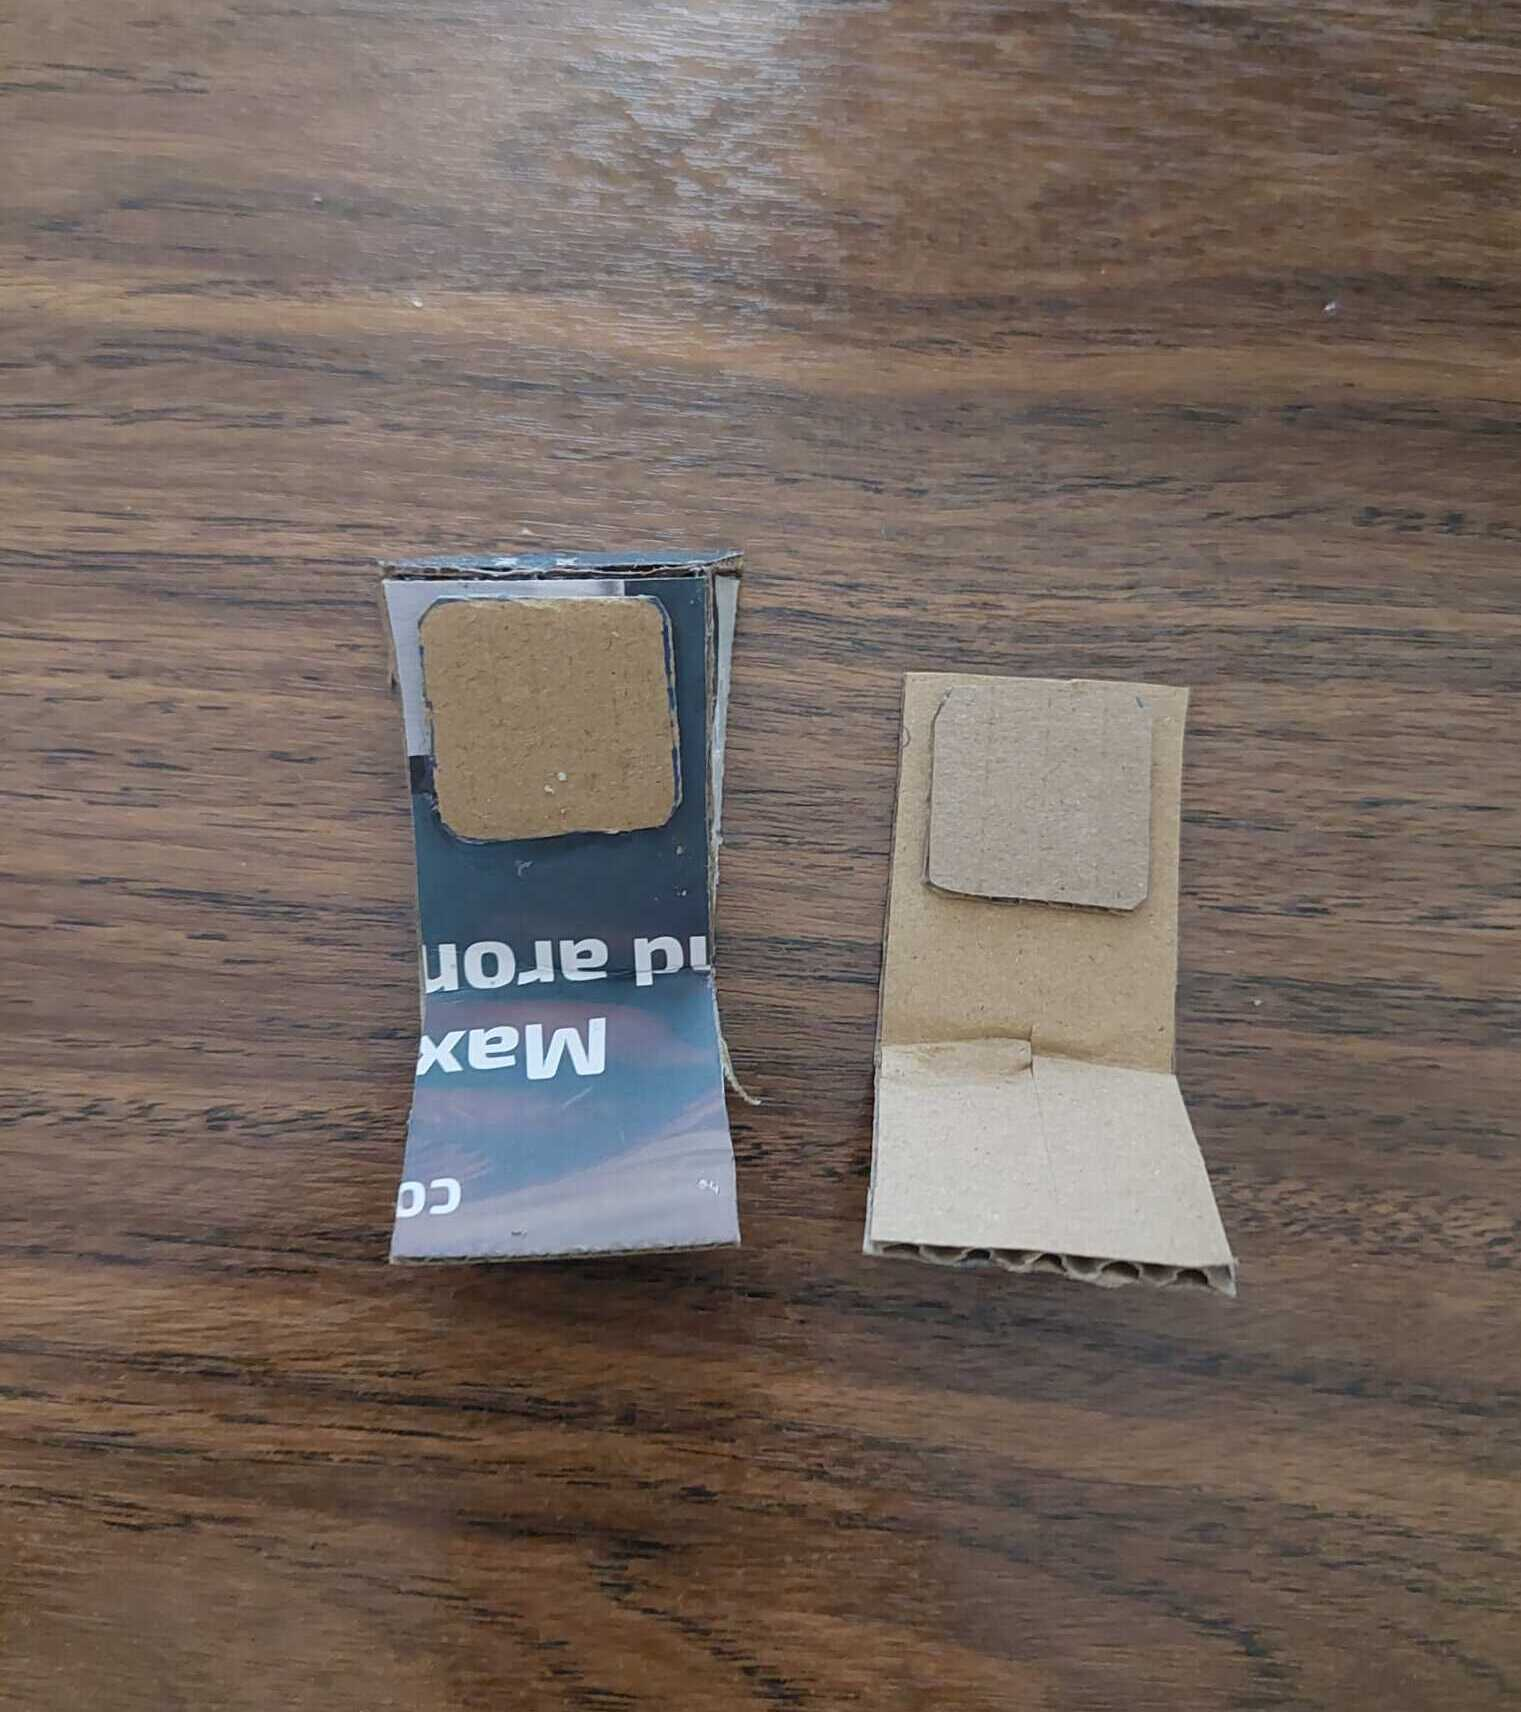
\includegraphics[width=\linewidth]{figs/cap5/boceto_carton4.jpeg}
		\caption*{\centering}
	\end{minipage}
	\hspace{2cm}
	\begin{minipage}{0.4\linewidth}
		\centering
		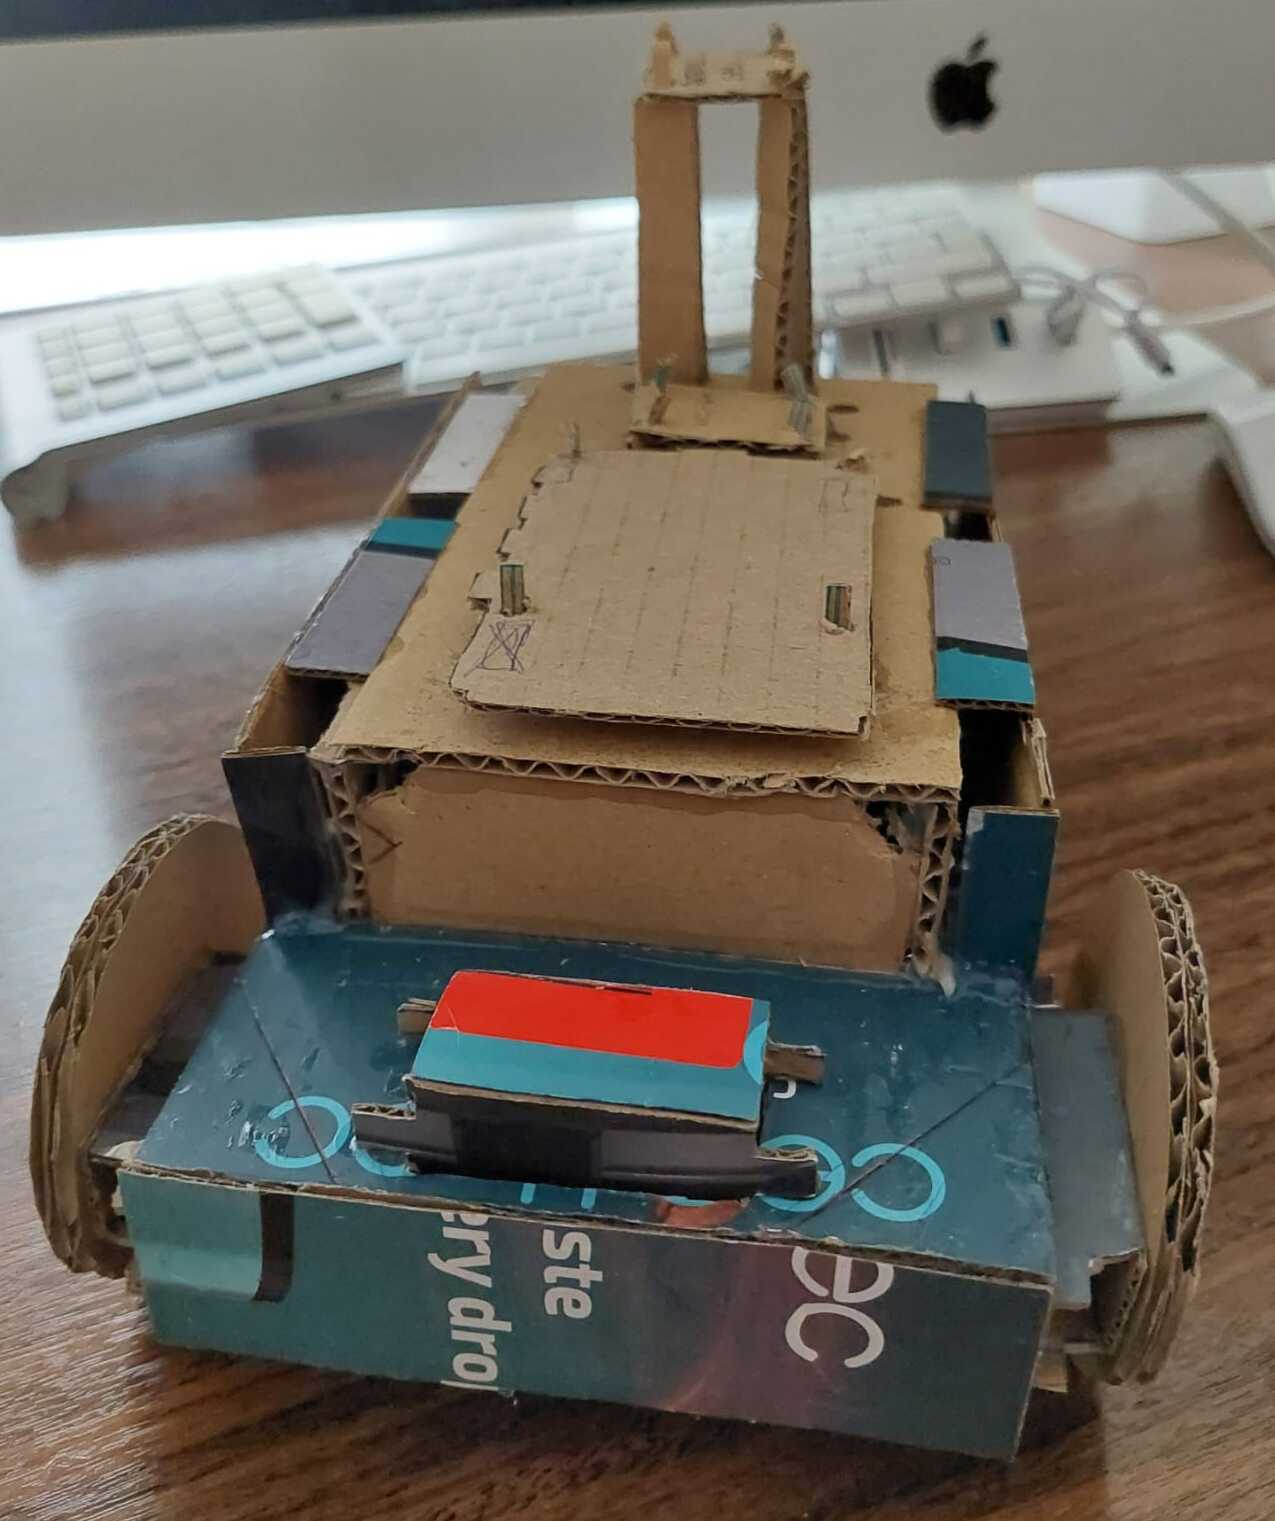
\includegraphics[width=\linewidth]{figs/cap5/boceto_carton5.jpeg}
		\caption*{\centering}
	\end{minipage}
	\hspace{2cm}
	\begin{minipage}{0.45\linewidth}
		\centering
		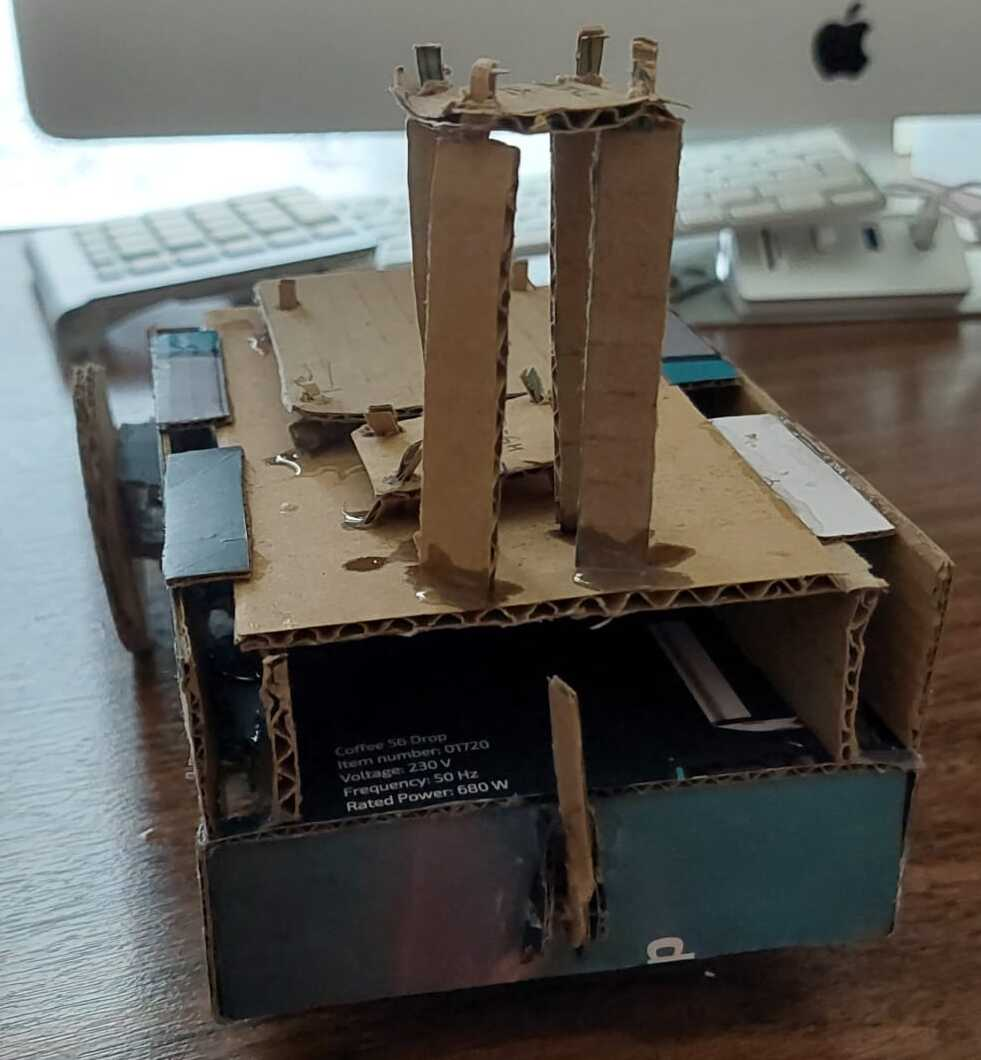
\includegraphics[width=\linewidth]{figs/cap5/boceto_carton6.jpeg}
		\caption*{\centering}
	\end{minipage}
	\hspace{2cm}
	\begin{minipage}{0.4\linewidth}
		\centering
		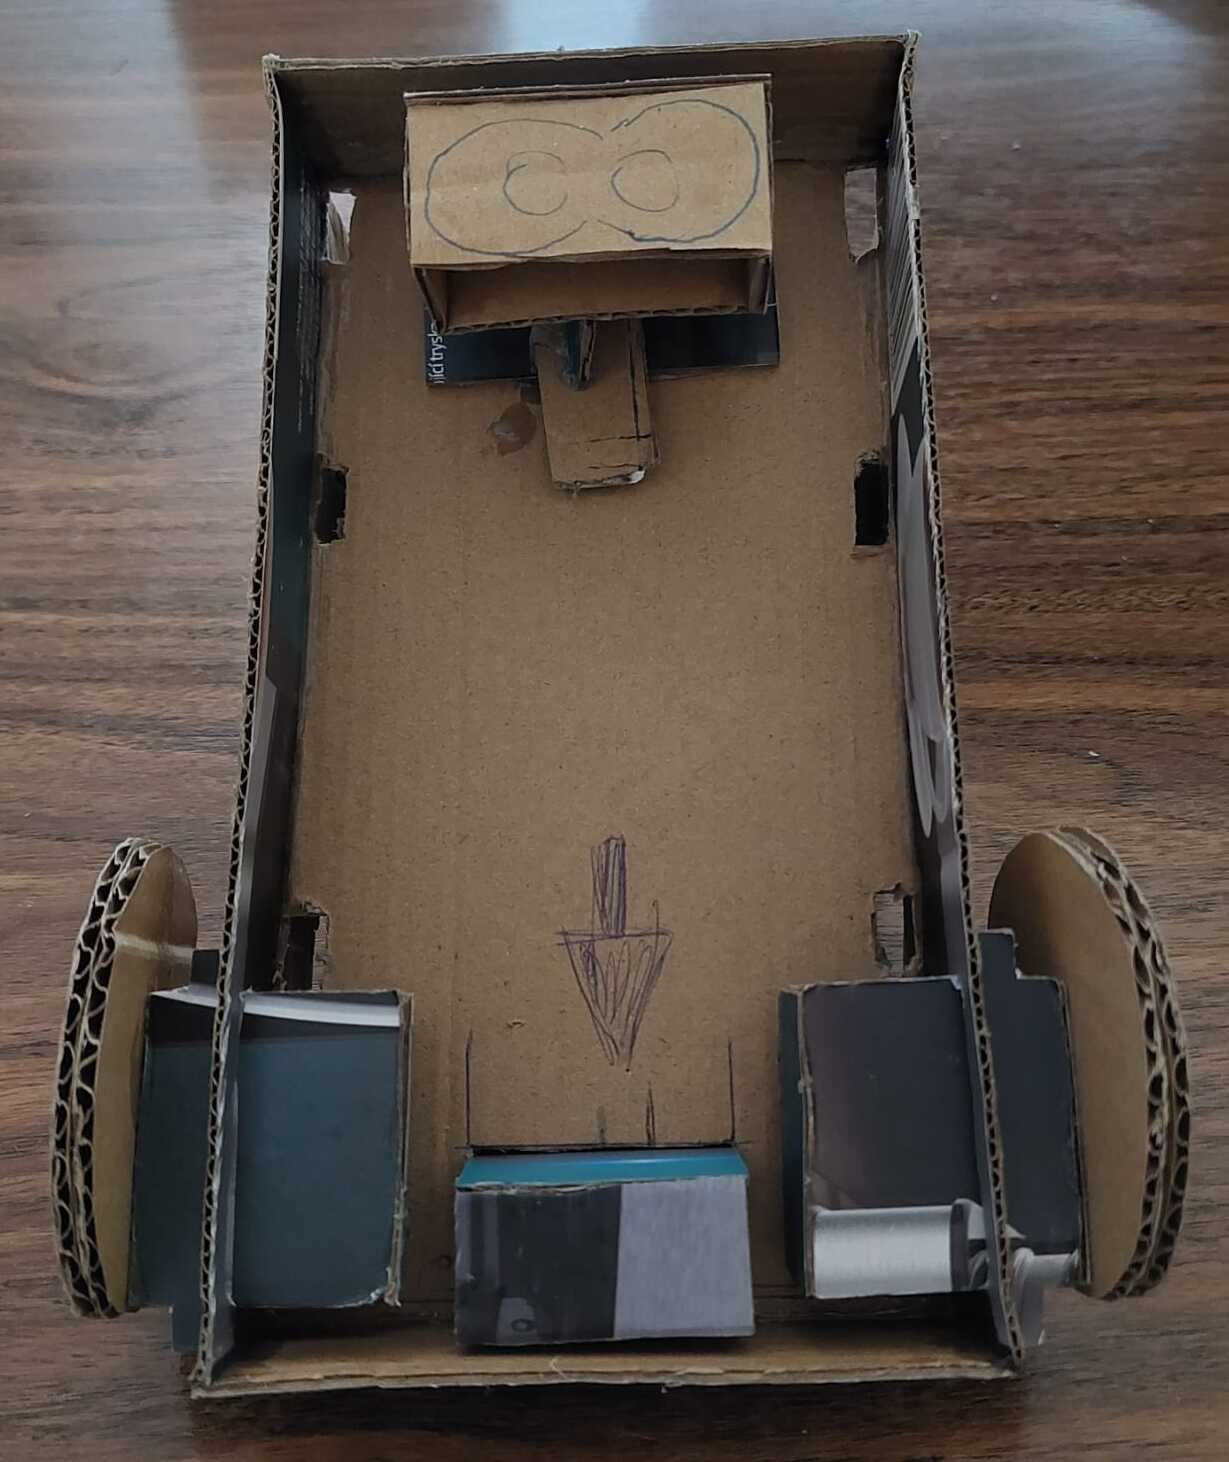
\includegraphics[width=\linewidth]{figs/cap5/boceto_carton7.jpeg}
		\caption*{\centering}
	\end{minipage}
	\caption{Maqueta final}
	\label{fig:maqueta2}
\end{figure}

Tras tener una idea clara de cómo va a ser Pibotj, es el momento de empezar a diseñar cada una de las piezas. 

\section{Diseño CAD}

Para hacer el diseño \acs{CAD} y la maqueta explicada en el apartado anterior, se crearon unos planos a mano (Figura \ref{fig:planos}) de las diferentes piezas que estarían involucradas en el diseño. Estas medidas son precisas gracias al uso del calibre (Figura \ref{fig:calibre}).


\begin{figure}[ht!]
	\centering
	\begin{minipage}{0.45\linewidth}
		\centering
		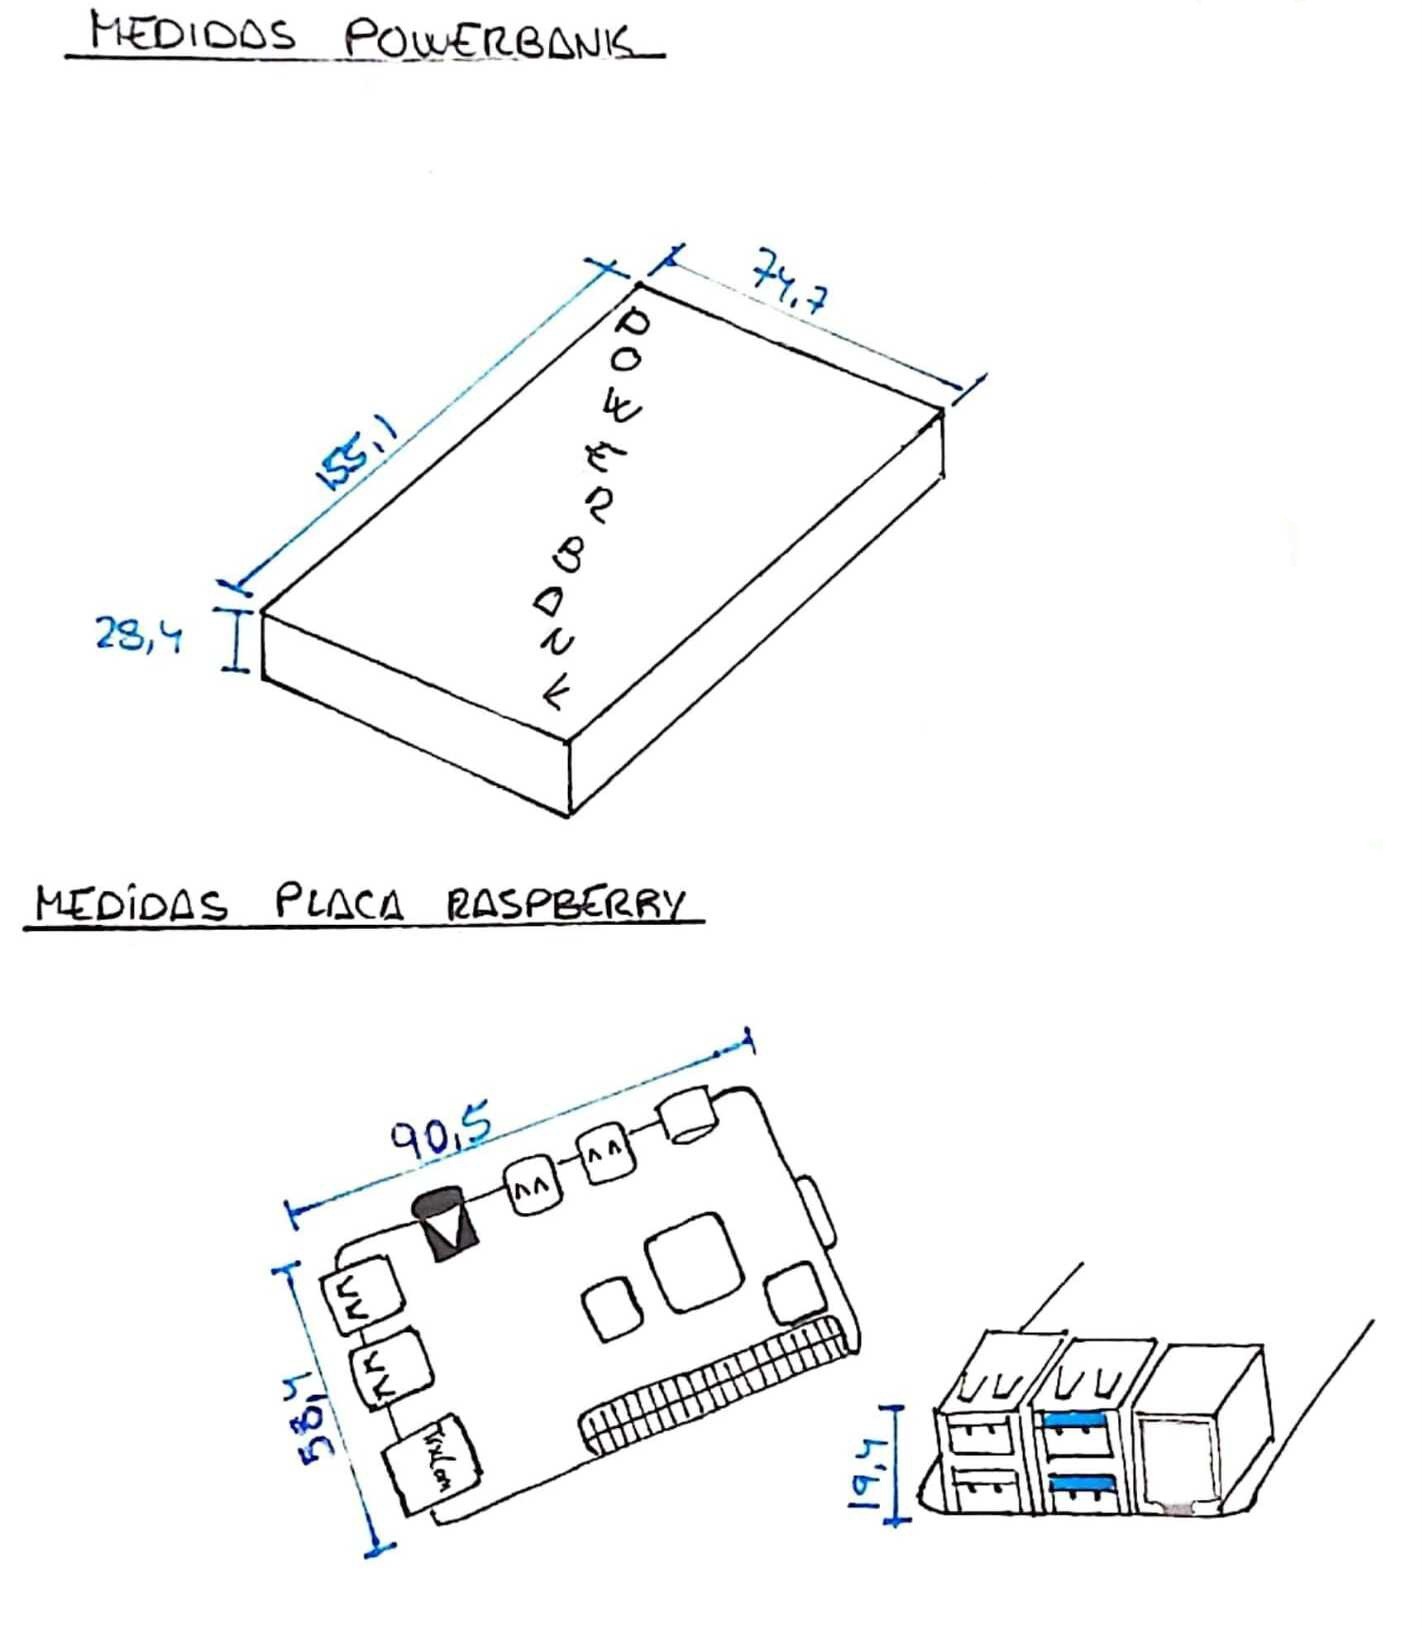
\includegraphics[width=\linewidth]{figs/cap5/planos1.jpeg}
		\caption*{\centering}
	\end{minipage}
	\hspace{1cm}
	\begin{minipage}{0.45\linewidth}
		\centering
		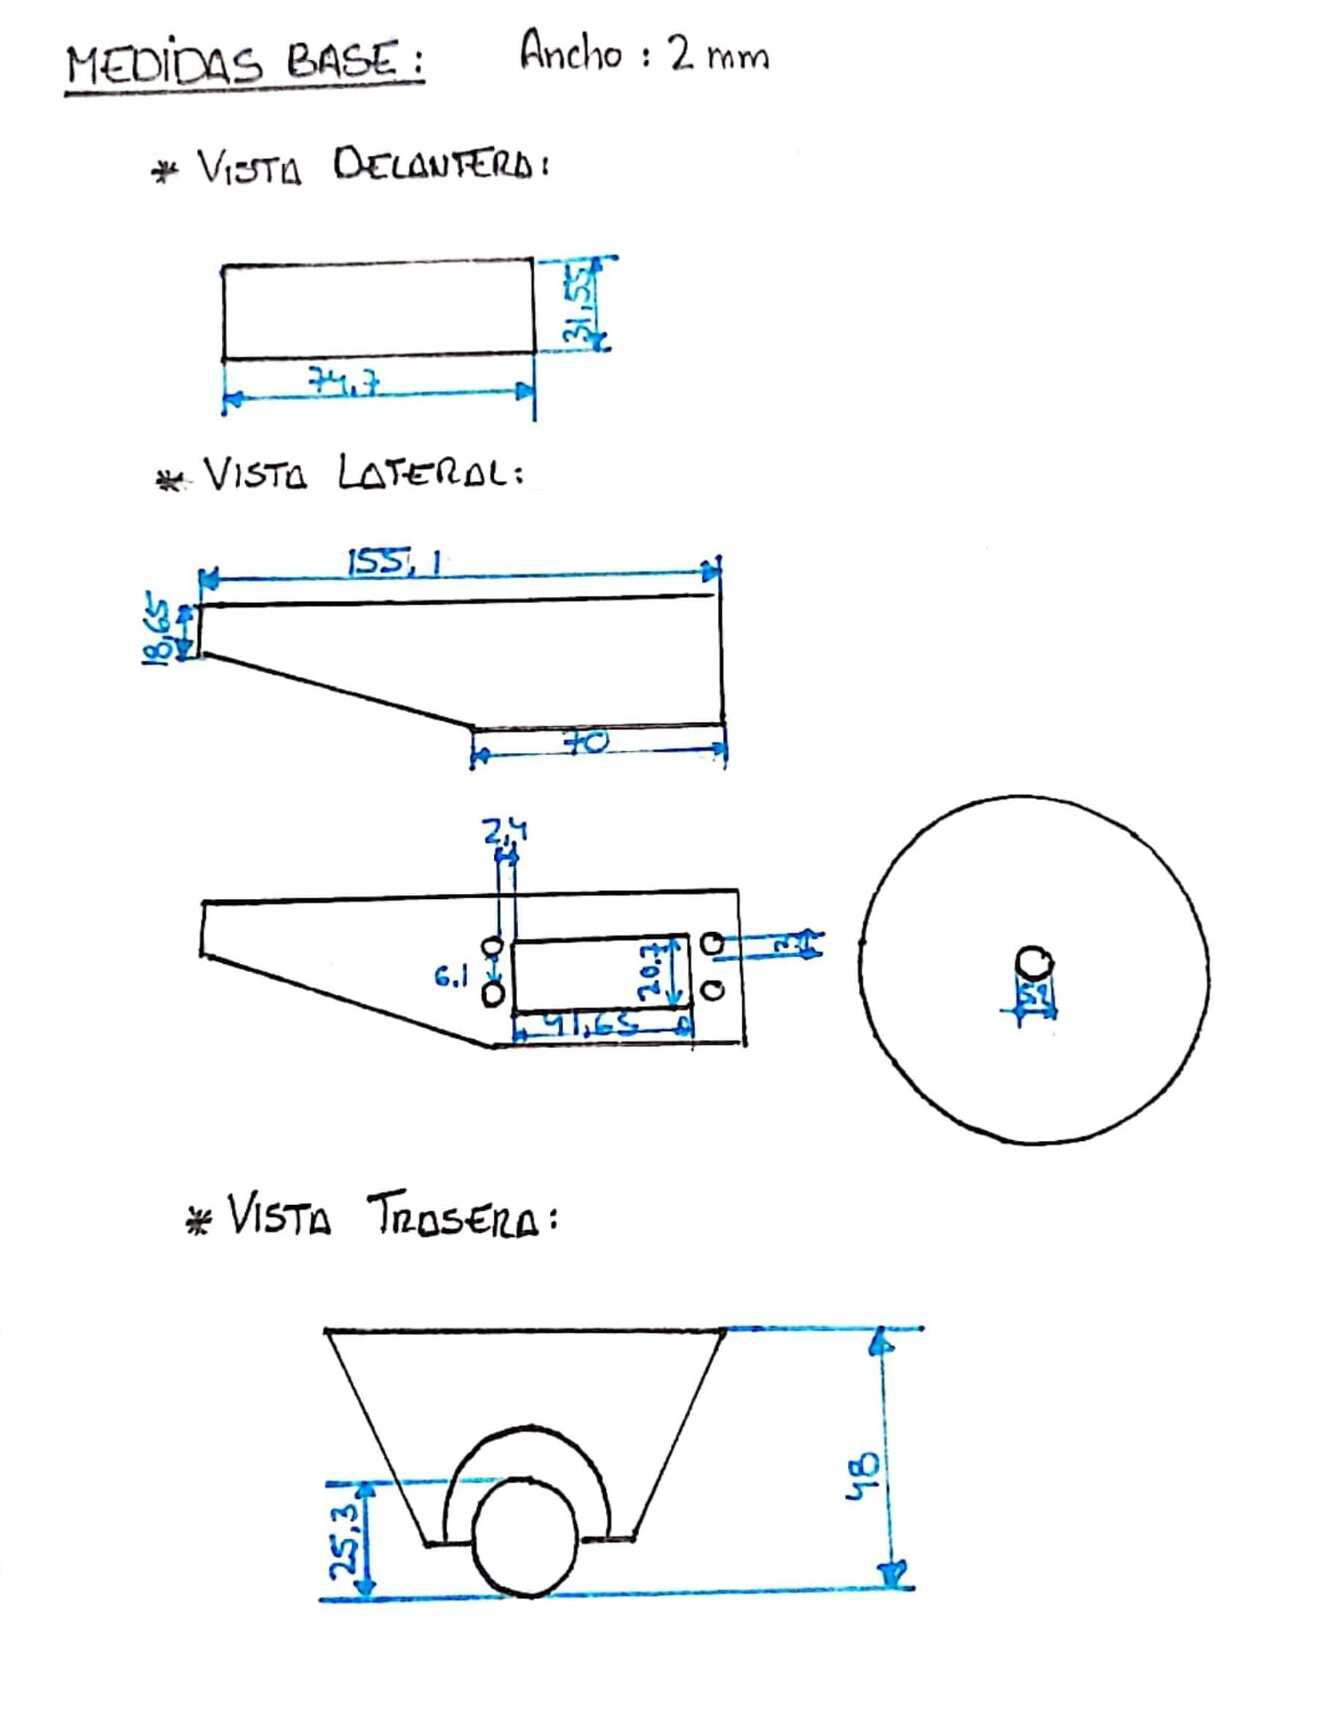
\includegraphics[width=\linewidth]{figs/cap5/planos2.jpeg}
		\caption*{\centering}
	\end{minipage}
	\hspace{1cm}
	\begin{minipage}{0.45\linewidth}
		\centering
		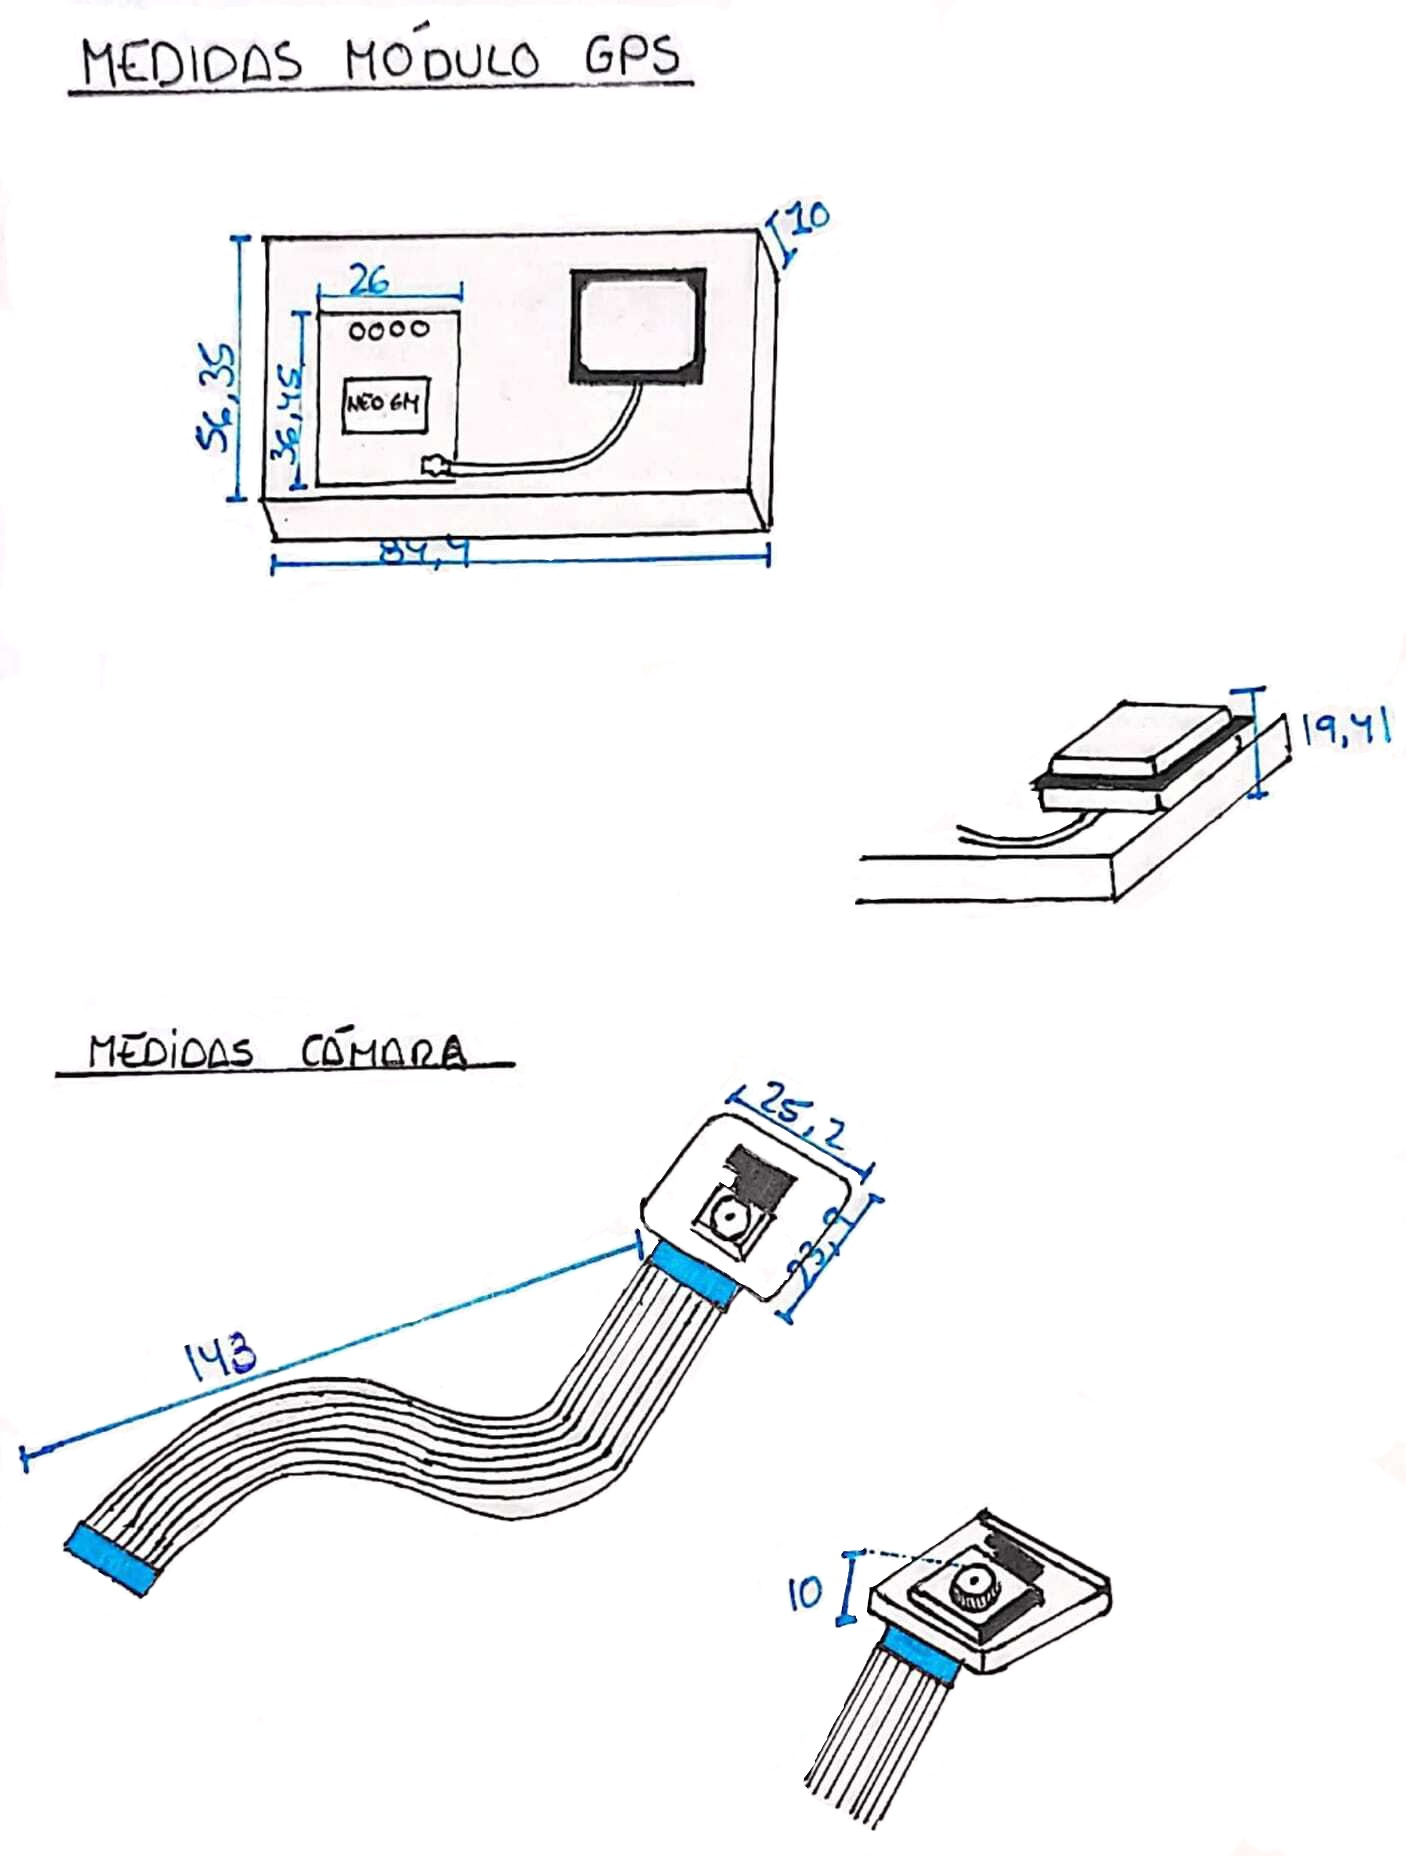
\includegraphics[width=\linewidth]{figs/cap5/planos3.jpeg}
		\caption*{\centering}
	\end{minipage}
	\hspace{1cm}
	\begin{minipage}{0.45\linewidth}
		\centering
		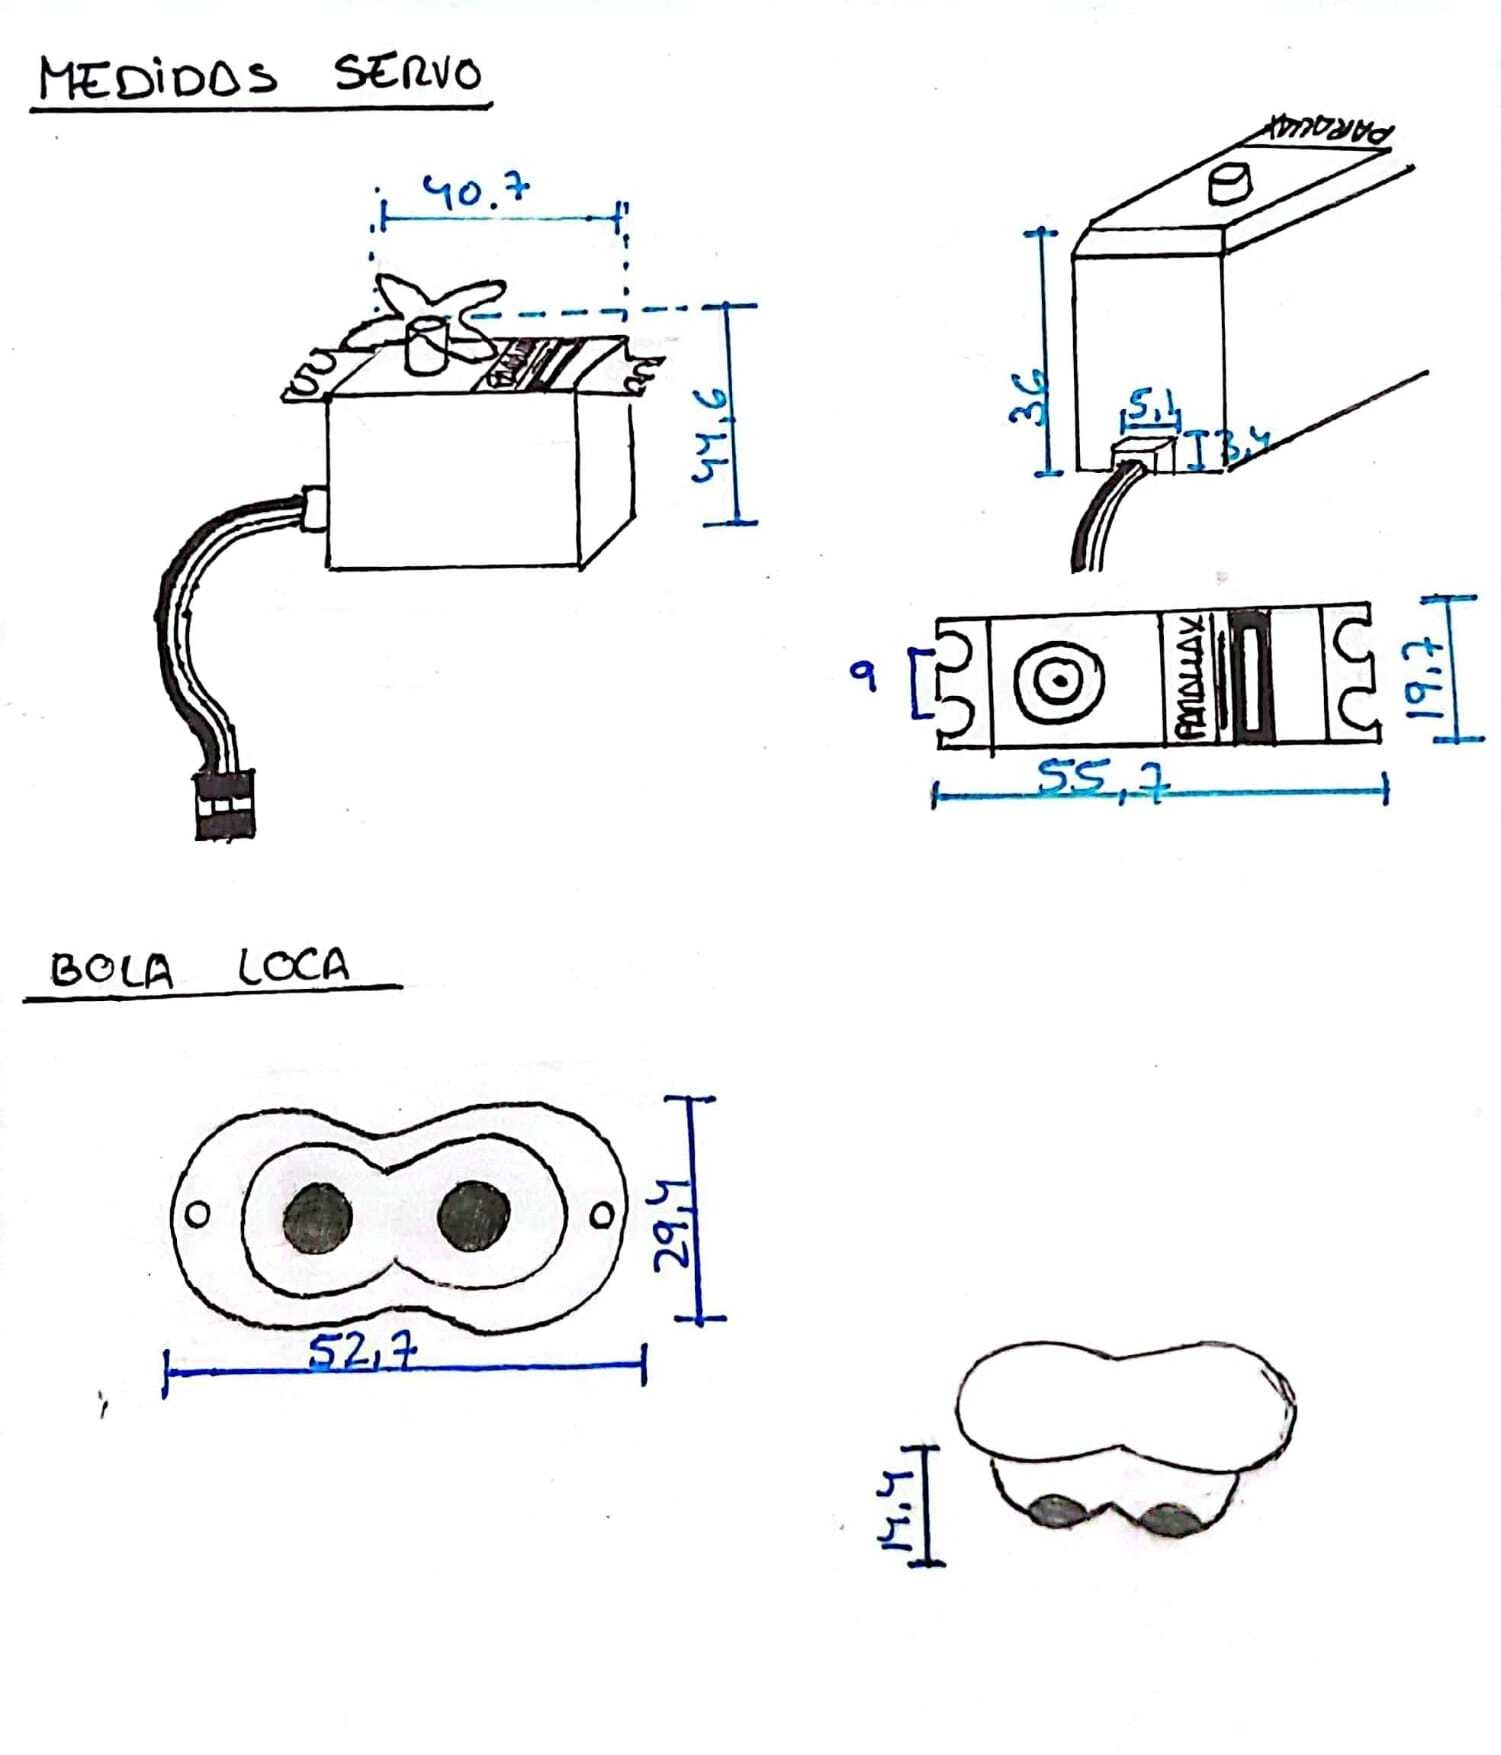
\includegraphics[width=\linewidth]{figs/cap5/planos4.jpeg}
		\caption*{\centering}
	\end{minipage}
	\caption{Planos de los componentes}
	\label{fig:planos}
\end{figure}


\begin{figure}[ht!]
	\centering
	\begin{minipage}{0.4\linewidth}
		\centering
		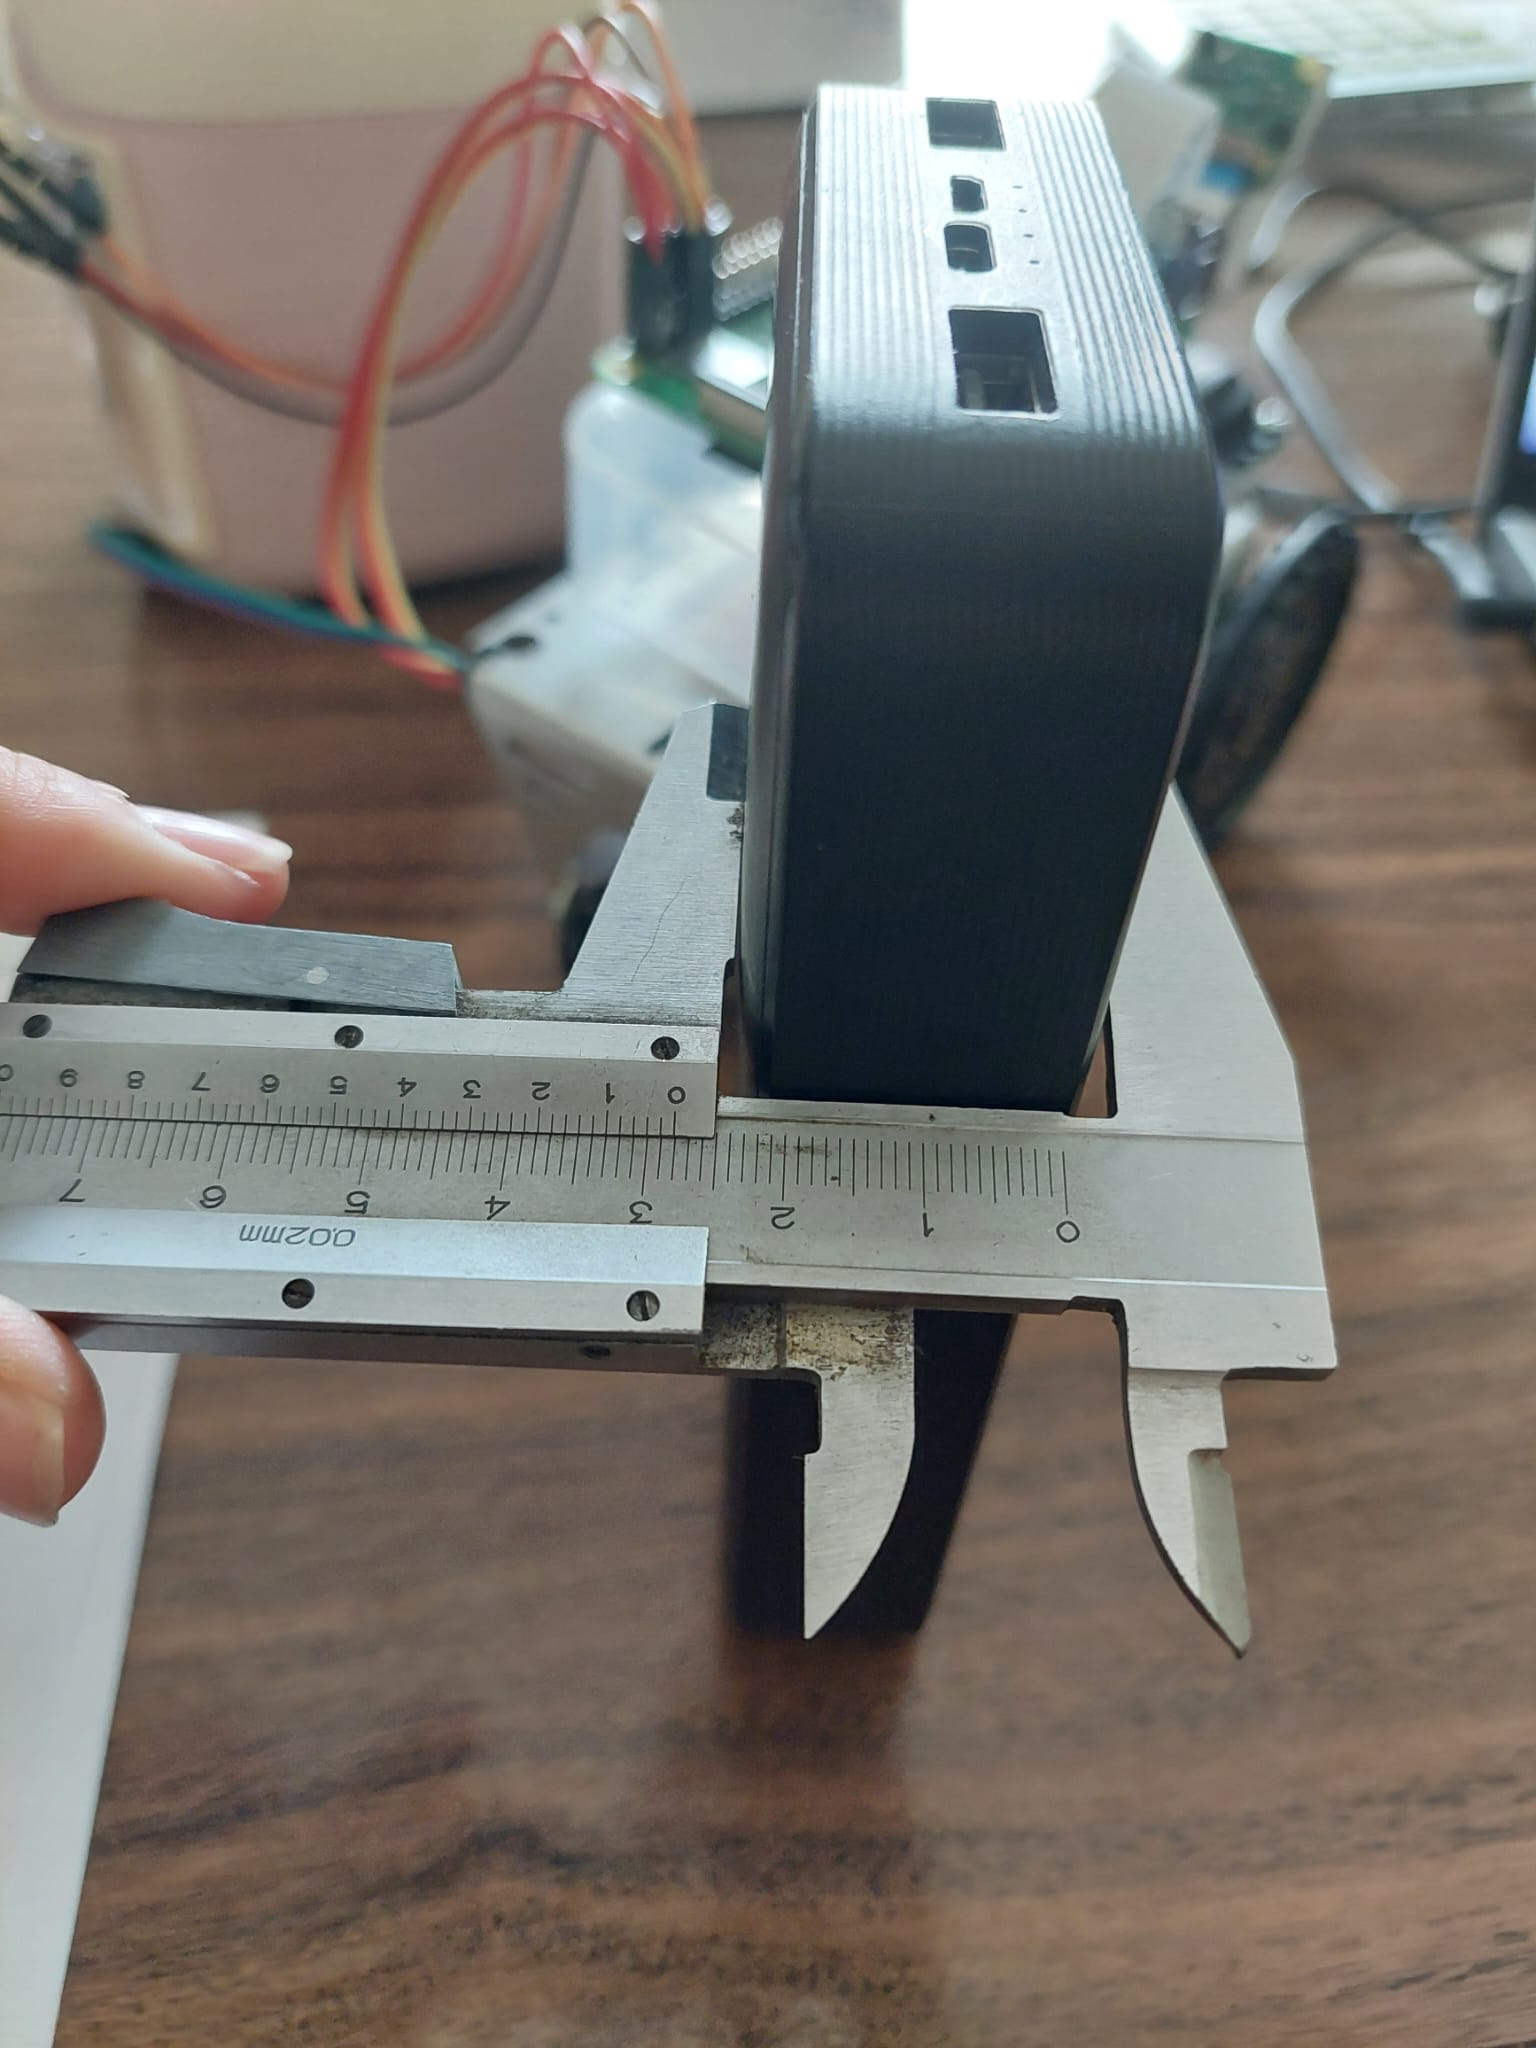
\includegraphics[width=\linewidth]{figs/cap5/calib1.jpeg}
		\caption*{\centering}
	\end{minipage}
	\hspace{2cm}
	\begin{minipage}{0.4\linewidth}
		\centering
		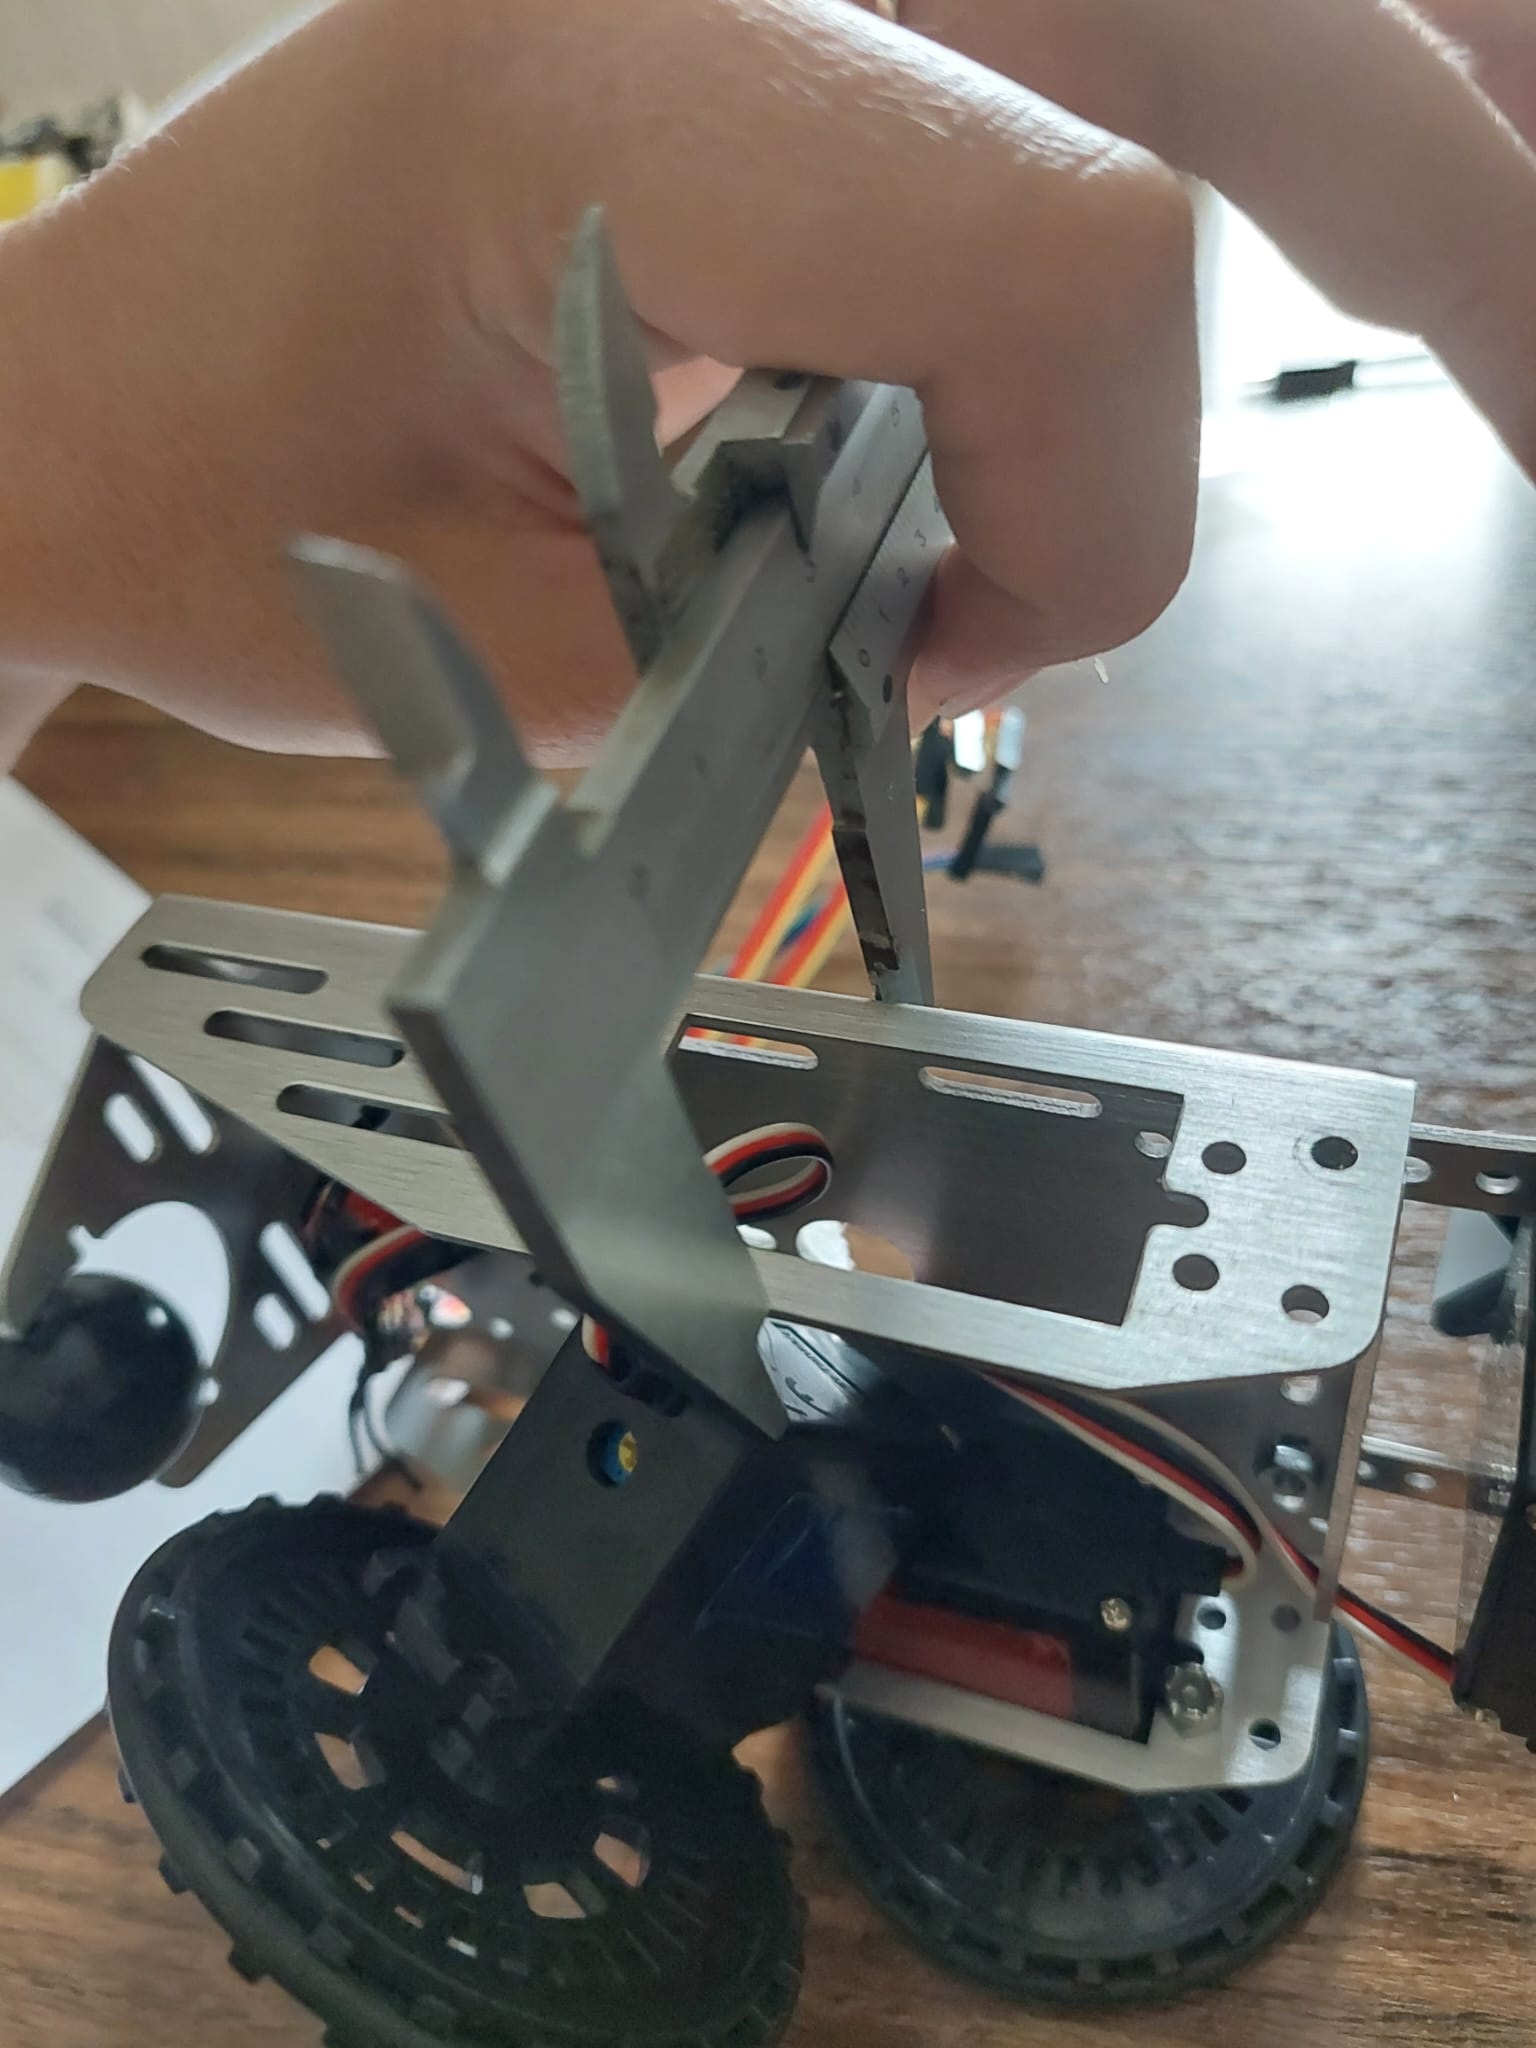
\includegraphics[width=\linewidth]{figs/cap5/calib2.jpeg}
		\caption*{\centering}
	\end{minipage}
	\caption{Usando el calibre}
	\label{fig:calibre}
\end{figure}

\setcounter{footnote}{65}

Para el diseño de Pibotj, se ha empleado la herramienta de modelado FreeCAD\footnote{\url{https://www.freecad.org/}} con el objetivo de utilizar \textit{software} libre, permitiendo que cualquier persona pueda acceder y modificar las piezas. El diseño se ha dividido en cuatro partes, cada una con una finalidad específica, las cuales se describirán a continuación.

Para llevar a cabo el diseño de todas las piezas, se han seguido los tutoriales de dos cursos de FreeCAD impartidos por Juan González (también conocido como Obijuan)\footnote{\url{https://www.youtube.com/watch?v=2_DbFzFV9D4&list=PLmnz0JqIMEzWQV-3ce9tVB_LFH9a91YHf}}, y el curso de FreeCAD para ingenieros de dcahue-ingeniería\footnote{\url{https://www.youtube.com/watch?v=4zp2DrWv8Wk&list=PLEpca2UUEwQeHp33w36SCzmCz_KKzaMKr&index=11}}, ambos fundamentales en el desarrollo del proyecto.

Además, se han utilizado otros tutoriales específicos, como los dedicados a la creación de \textit{shape binders}\footnote{\url{https://www.youtube.com/watch?v=MCY5IrWrHrU}} y la realización de planos inclinados\footnote{\url{https://www.youtube.com/watch?v=T4hKW1mLrCw}}, esenciales para diseñar la inclinación de la cámara.

\subsection{Pieza base}

La pieza base ha sido diseñada para alojar los motores de las ruedas y de la cámara. En la parte trasera, incorpora un prisma rectangular destinado a la colocación de la rueda loca, mientras que en el lado izquierdo cuenta con un orificio circular para sujetar la \textit{powerbank}. En la parte superior, se han añadido seis aberturas rectangulares para permitir el paso ordenado de los cables, manteniendo una estética limpia y organizada desde el exterior.

Además, dispone de cuatro orificios circulares que permiten fijar la pieza superior mediante tornillos. Se puede encontrar tanto su versión compatible con FreeCAD\footnote{\url{https://github.com/RoboticsURJC/tfg-jlopez/blob/main/design/base.FCStd}} como con el formato de diseño 3D por excelencia, STL\footnote{\url{https://github.com/RoboticsURJC/tfg-jlopez/blob/main/design/base.stl}}. La Figura \ref{fig:pbase} muestra la pieza base desde distintas perspectivas, tal como será preparada para la impresión en una impresora 3D convencional. Por su parte, la Figura \ref{fig:pbasemontada} presenta nuevamente la pieza base, pero esta vez equipada con los componentes de \textit{hardware} necesarios.

\begin{figure}[ht!]
	\centering
	\begin{minipage}{0.45\linewidth}
		\centering
		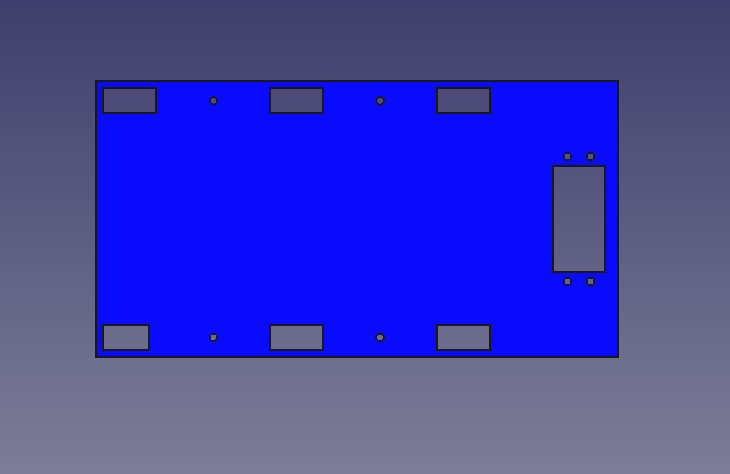
\includegraphics[width=\linewidth]{figs/cap5/basevistasuperiorsin.png}
		\caption*{\centering Vista superior}
	\end{minipage}
	\hspace{1cm}
	\begin{minipage}{0.45\linewidth}
		\centering
		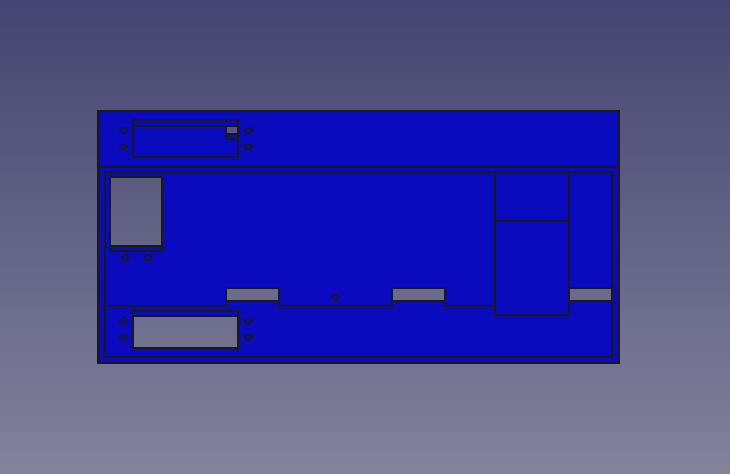
\includegraphics[width=\linewidth]{figs/cap5/basevistaladosin.png}
		\caption*{\centering Vista inferior}
	\end{minipage}
	\hspace{1cm}
	\begin{minipage}{0.45\linewidth}
		\centering
		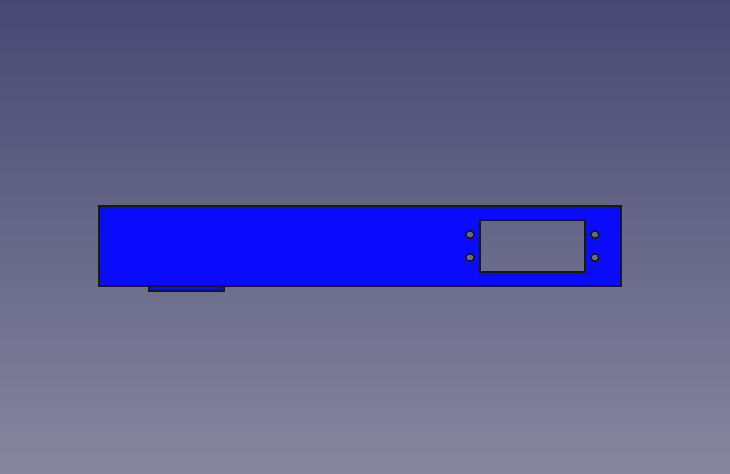
\includegraphics[width=\linewidth]{figs/cap5/basevistalateralsin.png}
		\caption*{\centering Vista lateral}
	\end{minipage}
	\hspace{1cm}
	\begin{minipage}{0.45\linewidth}
		\centering
		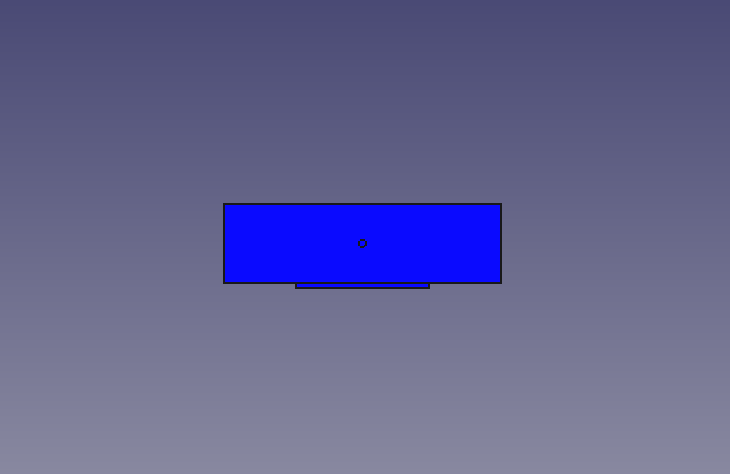
\includegraphics[width=\linewidth]{figs/cap5/basetraserasin.png}
		\caption*{\centering Vista lateral izquierdo}
	\end{minipage}

	\caption{Pieza base}
	\label{fig:pbase}
\end{figure}


\begin{figure}[ht!]
	\centering
	\begin{minipage}{0.45\linewidth}
		\centering
		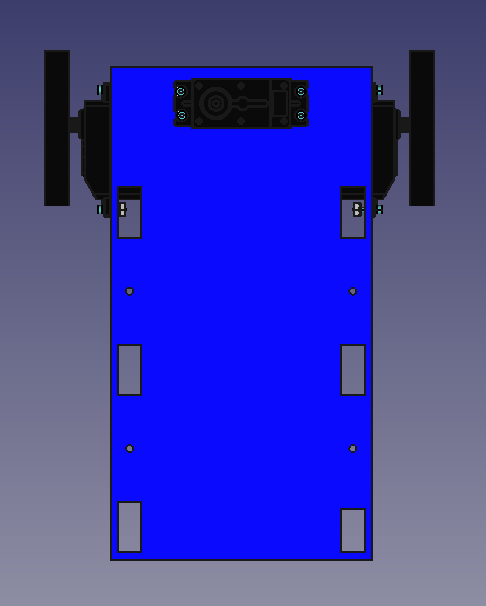
\includegraphics[width=\linewidth]{figs/cap5/basecon1.png}
		\caption*{\centering}
	\end{minipage}
	\hspace{1cm}
	\begin{minipage}{0.45\linewidth}
		\centering
		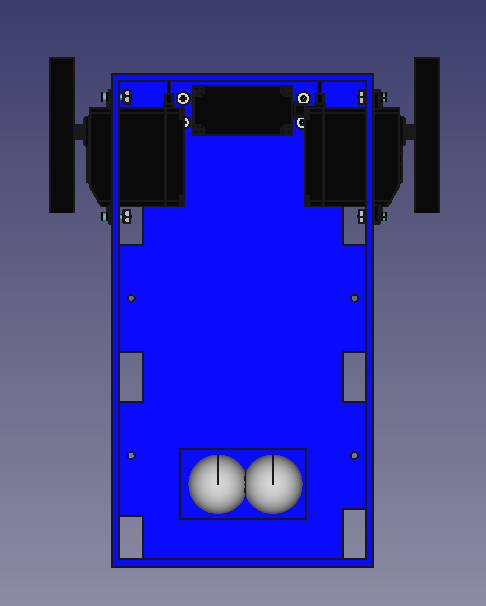
\includegraphics[width=\linewidth]{figs/cap5/basecon2.png}
		\caption*{\centering}
	\end{minipage}
	\caption{Pieza base atornillada}
	\label{fig:pbasemontada}
\end{figure}

\subsection{Pieza cámara}

 
Para posicionar la cámara de manera que mire hacia el suelo y pueda captar los baches, es necesario fijarla con una rotación sobre el eje y. En este caso, dicha rotación es de 50 grados, o 130 grados si se toma como referencia la base de la pieza que va atornillada al motor (Figura \ref{fig:rot}). Esta base cuenta con dos orificios diagonales que permiten su fijación al motor.

\begin{figure} [h!]
	\begin{center}
		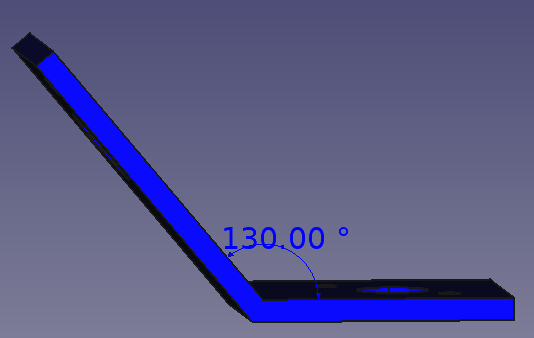
\includegraphics[width=8cm]{figs/cap5/rot.png}
	\end{center}
	\caption{Inclinación de la cámara} 
\label{fig:rot}
\end{figure}

La parte inclinada de la pieza incluye un orificio diseñado para alojar el sensor CMOS, garantizando una correcta alineación y visión. Además, esta sección tiene dos orificios adicionales para asegurar el sensor CMOS y mantenerlo firmemente en su lugar. Se puede encontrar tanto su versión compatible con FreeCAD\footnote{\url{https://github.com/RoboticsURJC/tfg-jlopez/blob/main/design/camara.FCStd}} como con el formato STL\footnote{\url{https://github.com/RoboticsURJC/tfg-jlopez/blob/main/design/camara.stl}}. La Figura \ref{fig:pcamara} muestra la pieza de la cámara desde distintas perspectivas, tal como será preparada para la impresión en una impresora 3D convencional. Por su parte, la Figura \ref{fig:pcamaramontada} presenta nuevamente la pieza de la cámara, pero esta vez atornillada sobre los componentes \textit{hardware} necesarios. 

\begin{figure}[ht!]
	\centering
	\begin{minipage}{0.45\linewidth}
		\centering
		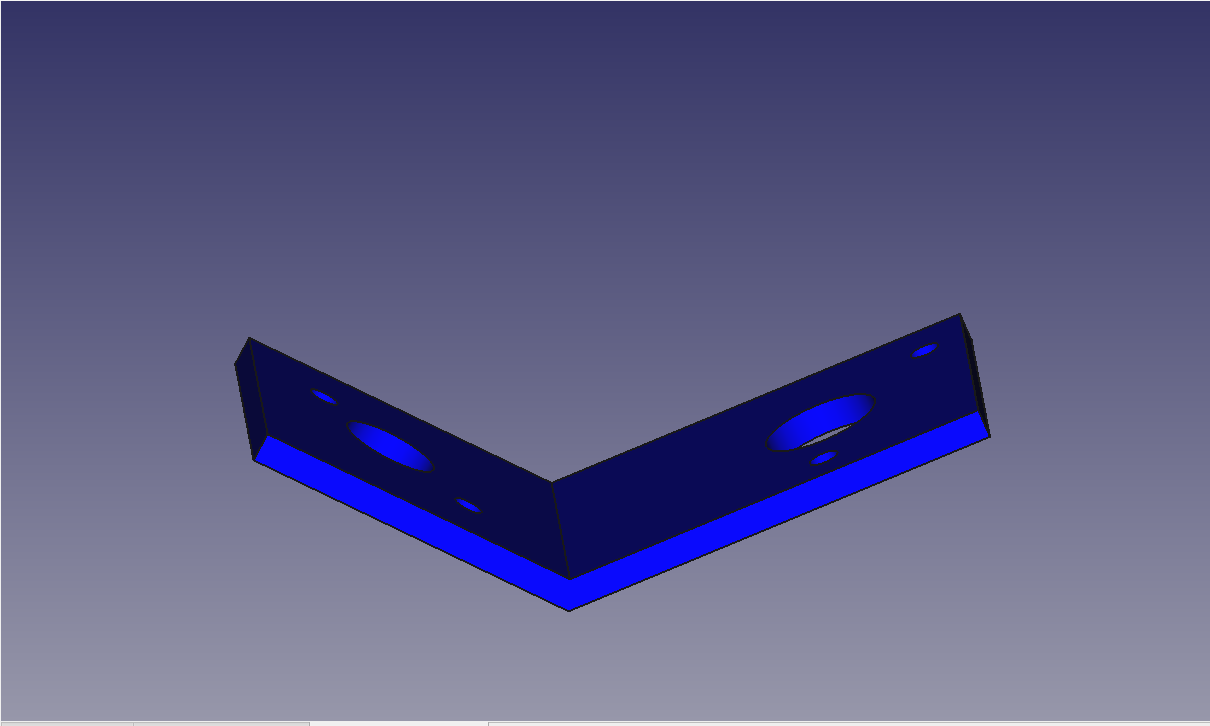
\includegraphics[width=\linewidth]{figs/cap5/camera2sin.png}
		\caption*{\centering}
	\end{minipage}
	\hspace{1cm}
	\begin{minipage}{0.45\linewidth}
		\centering
		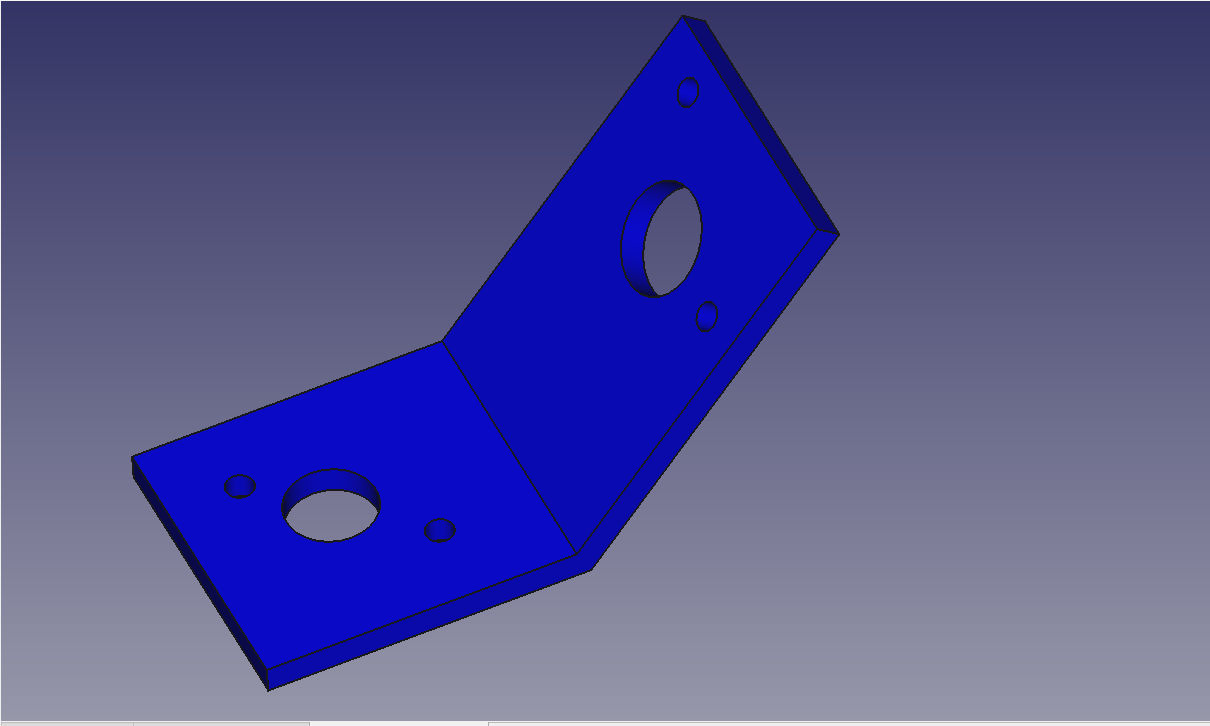
\includegraphics[width=\linewidth]{figs/cap5/camera3sin.png}
		\caption*{\centering}
	\end{minipage}
	
	\caption{Pieza cámara}
	\label{fig:pcamara}
\end{figure}


\begin{figure}[ht!]
	\centering
	\begin{minipage}{0.45\linewidth}
		\centering
		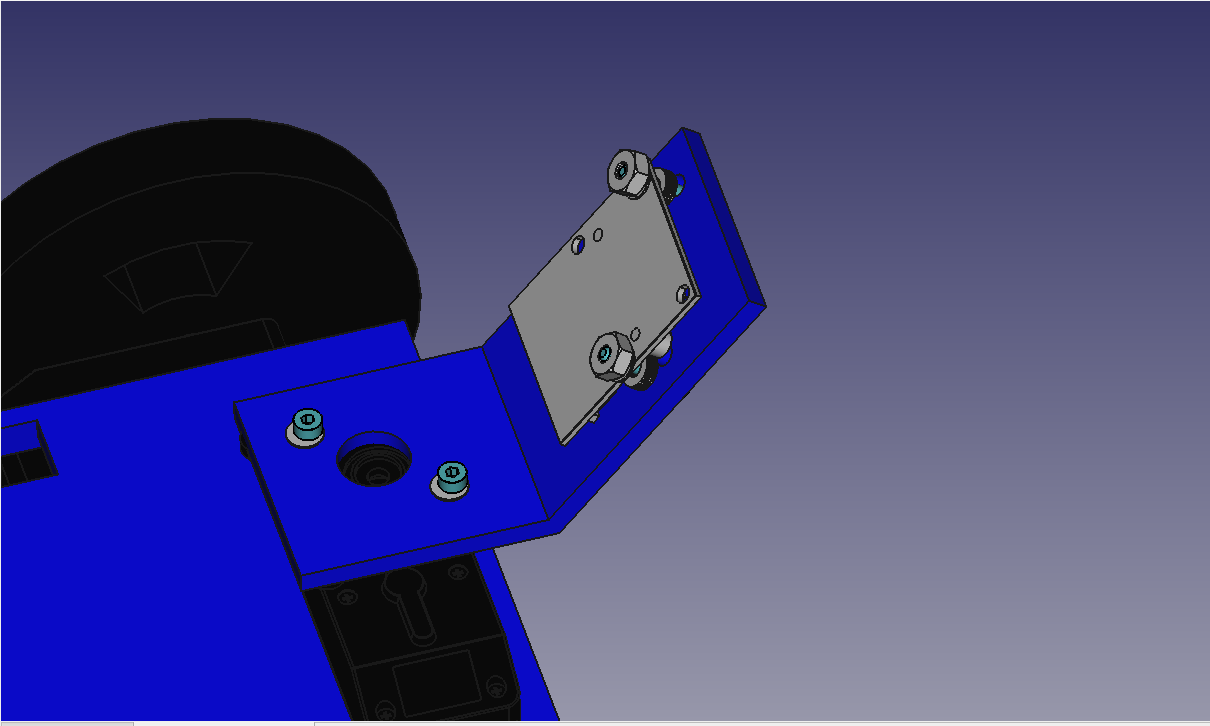
\includegraphics[width=\linewidth]{figs/cap5/camera2con.png}
		\caption*{\centering}
	\end{minipage}
	\hspace{1cm}
	\begin{minipage}{0.45\linewidth}
		\centering
		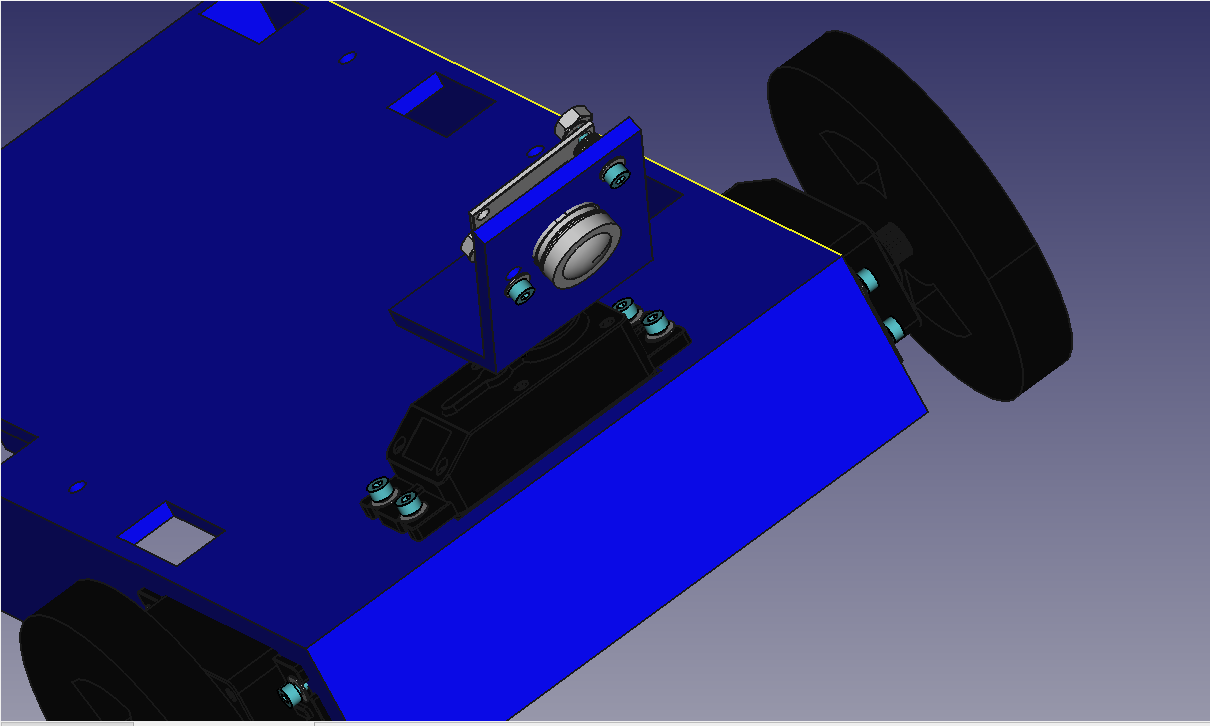
\includegraphics[width=\linewidth]{figs/cap5/camera3con.png}
		\caption*{\centering}
	\end{minipage}
	\caption{Pieza cámara atornillada}
	\label{fig:pcamaramontada}
\end{figure}


\subsection{Pieza superior}


Esta pieza superior ha sido diseñada para alojar la placa Raspberry Pi, el módulo GPS y la \textit{powerbank} en su interior. En la cara superior se encuentran doce orificios circulares destinados a atornillar tanto la Raspberry Pi como el módulo GPS. Además, en esta misma cara hay seis aberturas que se conectan con la cara inferior, alineándose con las aberturas correspondientes de la pieza base para garantizar un paso de cables ordenado.

La cara inferior, además de las seis aberturas, incluye cuatro orificios adicionales para permitir el atornillado de la pieza base. En el lateral izquierdo, la pieza está abierta para facilitar la inserción de la \textit{powerbank}, mientras que en el lado derecho cuenta con dos cuadrantes que permiten retirar la \textit{powerbank} cuando sea necesario. Esta pieza está disponible tanto en formato compatible con FreeCADL\footnote{\url{https://github.com/RoboticsURJC/tfg-jlopez/blob/main/design/parte-superior.FCStd}} como en STL\footnote{\url{https://github.com/RoboticsURJC/tfg-jlopez/blob/main/design/parte-superior.stl}}.

La Figura \ref{fig:psuperior} muestra la pieza base desde varias perspectivas, lista para la impresión en una impresora 3D convencional. La Figura \ref{fig:psuperiormontada} presenta nuevamente la pieza base, pero equipada con los componentes de hardware necesarios.


\begin{figure}[ht!]
	\centering
	\begin{minipage}{0.45\linewidth}
		\centering
		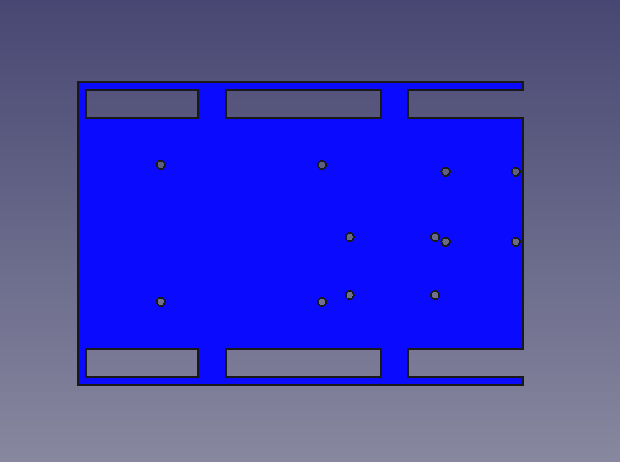
\includegraphics[width=\linewidth]{figs/cap5/superior1.png}
		\caption*{\centering Vista superior}
	\end{minipage}
	\hspace{1cm}
	\begin{minipage}{0.45\linewidth}
		\centering
		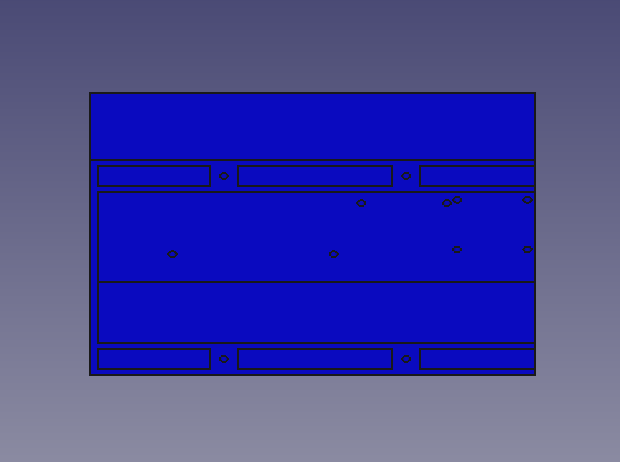
\includegraphics[width=\linewidth]{figs/cap5/superior2.png}
		\caption*{\centering Vista inferior}
	\end{minipage}
	\hspace{1cm}
	\begin{minipage}{0.45\linewidth}
		\centering
		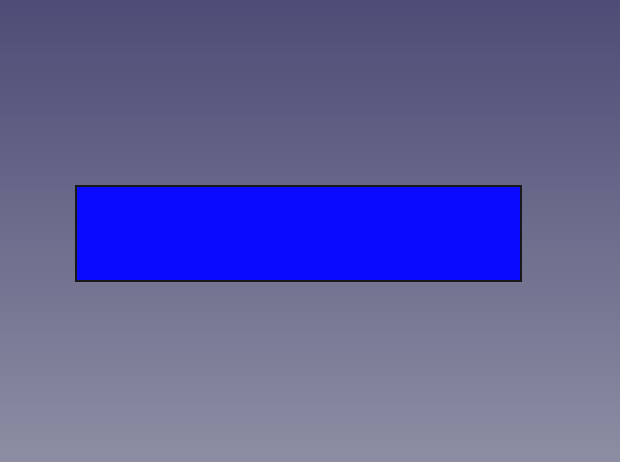
\includegraphics[width=\linewidth]{figs/cap5/superior3.png}
		\caption*{\centering Vista lateral}
	\end{minipage}
	\hspace{1cm}
	\begin{minipage}{0.45\linewidth}
		\centering
		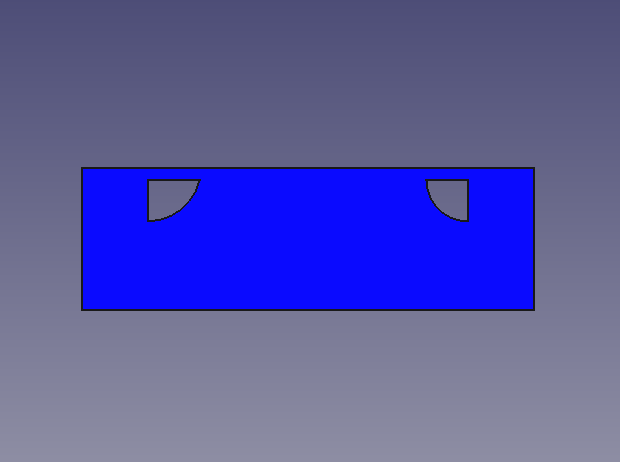
\includegraphics[width=\linewidth]{figs/cap5/superior4.png}
		\caption*{\centering Vista lateral izquierdo}
	\end{minipage}
	
	\caption{Pieza superior}
	\label{fig:psuperior}
\end{figure}


\begin{figure}[ht!]
	\centering
	\begin{minipage}{0.45\linewidth}
		\centering
		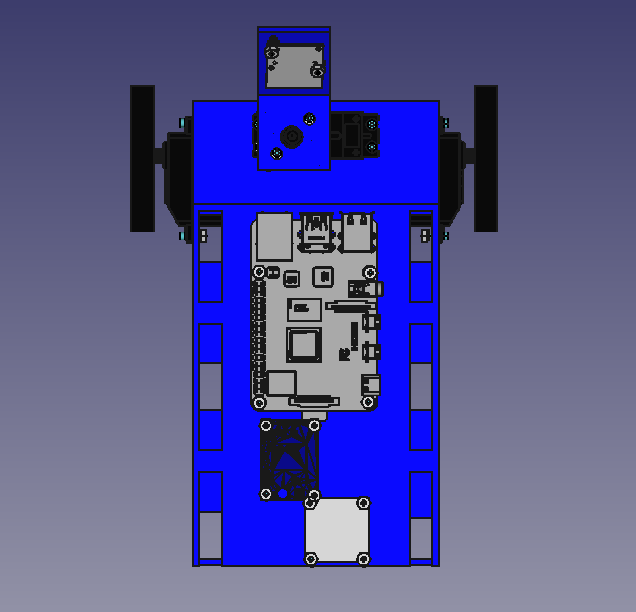
\includegraphics[width=\linewidth]{figs/cap5/superior1m.png}
		\caption*{\centering}
	\end{minipage}
	\hspace{1cm}
	\begin{minipage}{0.45\linewidth}
		\centering
		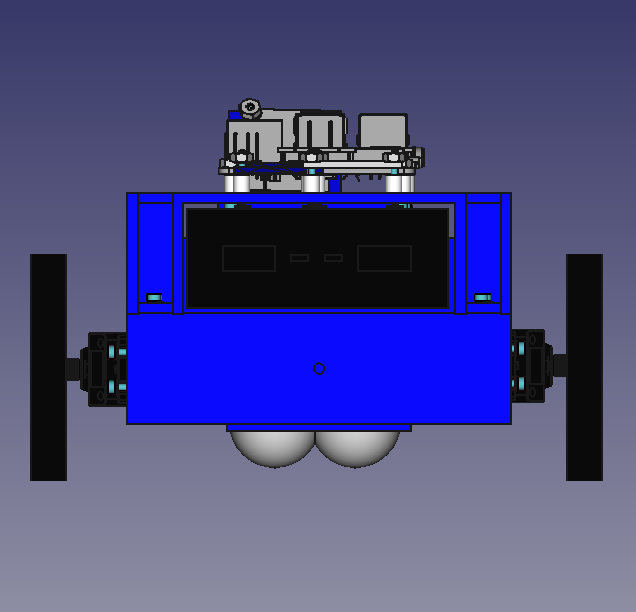
\includegraphics[width=\linewidth]{figs/cap5/superior2m.png}
		\caption*{\centering}
	\end{minipage}
	\caption{Pieza superior atornillada}
	\label{fig:psuperiormontada}
\end{figure}


\subsection{Pieza sujección trasera}

Para asegurar que la \textit{powerbank} se mantenga en su lugar dentro del robot, se ha diseñado una pieza que se atornilla en el lado izquierdo de la base. Esta pieza es un prisma rectangular con más de 30 mm de altura, aproximadamente 5 mm de largo y 3 mm de ancho (Figura \ref{fig:ptrasera}). Su función es mantener la \textit{powerbank} en su hueco. La pieza debe colocarse en posición vertical para evitar que la \textit{powerbank} se deslice, y en posición horizontal cuando se desee retirarla. Existe una versión en FreeCAD\footnote{\url{https://github.com/RoboticsURJC/tfg-jlopez/blob/main/design/sujeccion-trasera.FCStd}} y otra en formato STL\footnote{\url{https://github.com/RoboticsURJC/tfg-jlopez/blob/main/design/sujeccion-trasera.stl}}. La Figura \ref{fig:traseracon} muesta cómo quedaría montada la pieza sobre el robot.

\begin{figure}[ht!]
	\centering
	\begin{minipage}{0.45\linewidth}
		\centering
		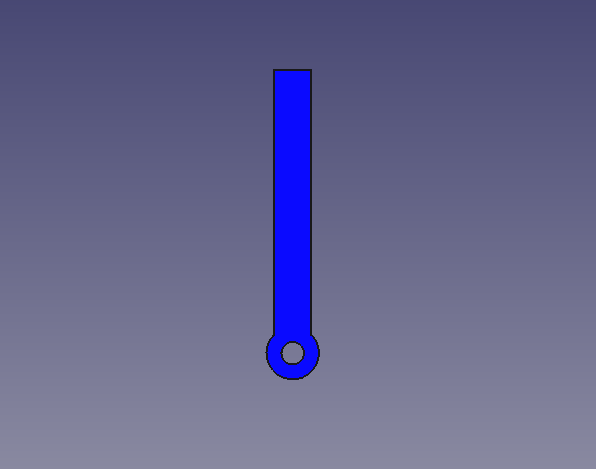
\includegraphics[width=\linewidth]{figs/cap5/trasera1.png}
		\caption*{\centering}
	\end{minipage}
	\hspace{1cm}
	\begin{minipage}{0.45\linewidth}
		\centering
		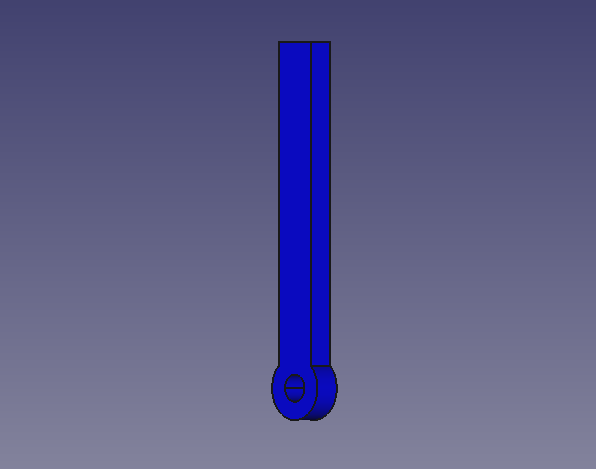
\includegraphics[width=\linewidth]{figs/cap5/trasera2.png}
		\caption*{\centering}
	\end{minipage}
	\caption{Pieza sujección trasera}
	\label{fig:ptrasera}
\end{figure}

\begin{figure} [h!]
	\begin{center}
		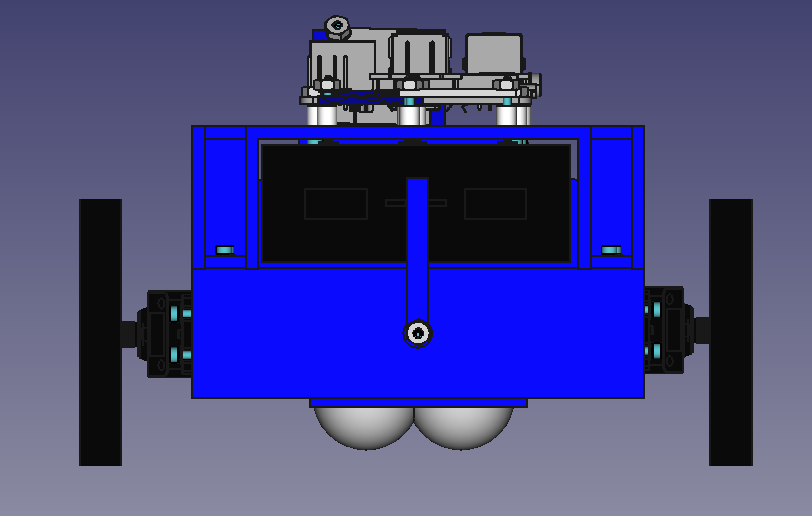
\includegraphics[width=8cm]{figs/cap5/traseracon.png}
	\end{center}
	\caption{Pieza sujección trasera montada} 
	\label{fig:traseracon}
\end{figure}

Una vez detalladas cada una de las piezas \acs{CAD} diseñadas, es momento de describir el proceso de impresión y montaje que se ha seguido para obtener a Pibotj.
  
\section{Impresión y montaje}

En esta sección se presentan todos los detalles que deben considerarse para replicar este proyecto. 

Para la impresión de Pibotj se ha usado la impresora FDM Creality Ender3 V2 (Figura \ref{fig:impresora}), un rollo de PLA convencional azul y Ultimaker Cura\footnote{\url{https://ultimaker.com/es/software/ultimaker-cura/}} como \textit{software} de impresión. Se ha usado para la impresión de todas las piezas las características que muestra el Cuadro \ref{cuadro:cimpresion}. En este proyecto es necesario imprimir una pieza de cada una explicada en el apartado de Diseño CAD, como muestra la Figura \ref{fig:piezasimpresas}. La duración de impresión es en torno a 50 horas.
 
\begin{figure} [h!]
	\begin{center}
		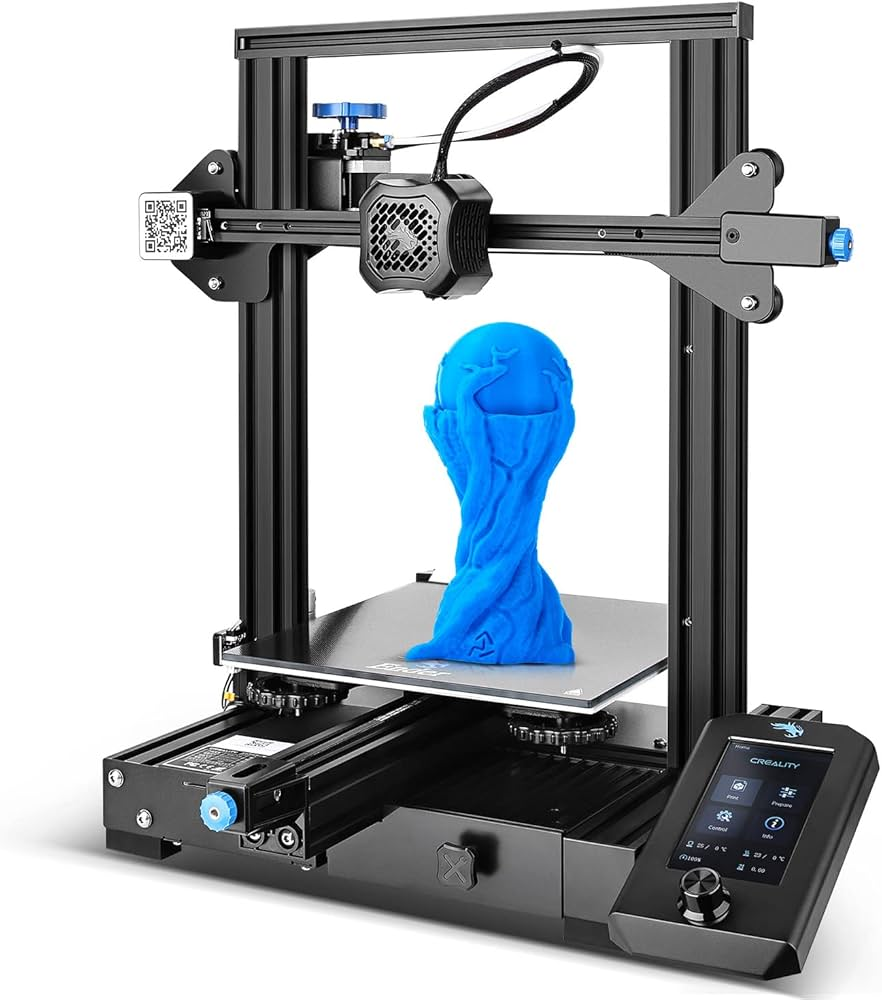
\includegraphics[width=7cm]{figs/cap5/impresora.jpg}
	\end{center}
	\caption{Impresora FDM Creality Ender3 V2$^{\ref{note:enlace80}}$} 
	\label{fig:impresora}
\end{figure}

\setcounter{footnote}{80} % Establecer la numeración de la siguiente nota al pie
\footnotetext[\value{footnote}]{\url{https://www.creality.com/es/products/ender-3-v2-neo-3d-printer}\label{note:enlace80}}

\begin{table}[H]
	\begin{center}
		\begin{tabular}{|c|c|}
			\hline
			Características & Parámetros\\
			\hline
			\multirow{2}{*}{Calidad} & \multirow{2}{*}{\shortstack{ Altura de capa: 0,2 mm \\ Ancho de línea: 0.4 mm}}\\
			& \\
			\hline
			\multirow{4}{*}{Paredes} & \multirow{4}{*}{\shortstack{Grosor de pared: 0,8 mm \\ Cantidad de líneas de pared: 2 \\ Alineación de costura en Z: \textit{Esquina más afilada} \\ Preferencia de costura en esquina: \textit{Ocultación inteligente} }} \\
			& \\
			& \\
			& \\
			\hline
			
			\multirow{2}{*}{\shortstack{Relleno}} &  \multirow{2}{*}{\shortstack{Densidad de relleno: 15\% \\ Patrón de relleno: \textit{Gyroid} }}\\
			& \\
			\hline
			\multirow{2}{*}{\shortstack{Velocidad}} &  \multirow{2}{*}{\shortstack{Velocidad de impresión: 50 mm/s\\ Velocidad de la primera capa: 20 mm/s}}\\
			& \\
			\hline
		\end{tabular}
		\caption{Características usadas para la impresión}
		\label{cuadro:cimpresion}
	\end{center}
\end{table}


\begin{figure} [h!]
	\begin{center}
		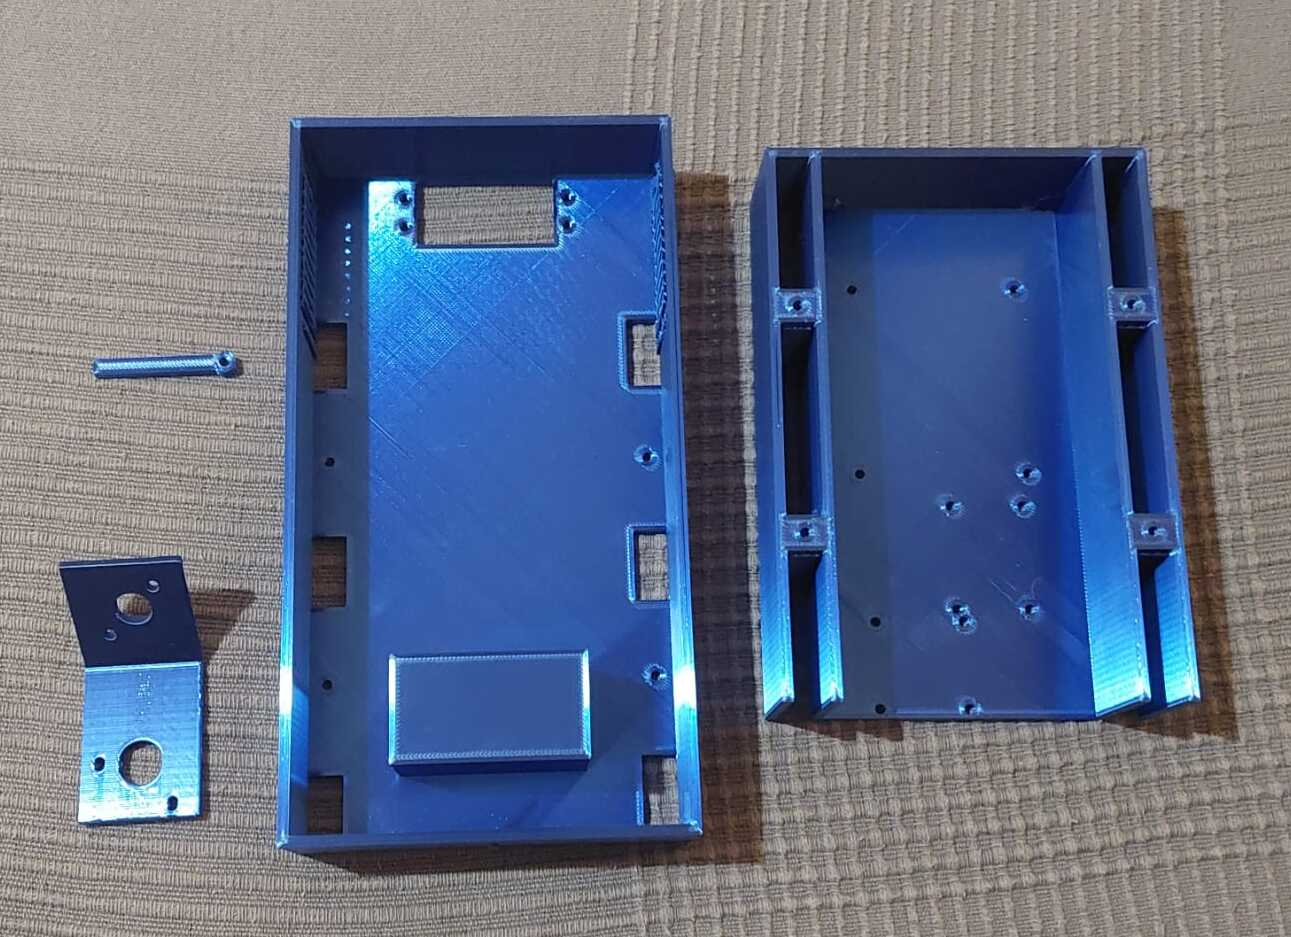
\includegraphics[width=10cm]{figs/cap5/setcompleto.jpeg}
	\end{center}
	\caption{Piezas impresas} 
	\label{fig:piezasimpresas}
\end{figure}


Una vez impresas todas las piezas y retirado sus soportes generados, es el momento del montaje; cuya duración es de dos horas aproximadamente, dependiendo de las habilidades del usuario.

Uno de los elementos a tener en cuenta para el montaje son los Hama Beads (Figura \ref{fig:hamabeads}). Los Hama Beads son cilindros de plástico pequeños con un círulo en el centro usados comunmente para manualidades y para la creación de objetos de decoración. En este caso, se ha usado para evitar que tanto la Raspberry Pi como el módulo GPS toquen directamente la superficie impresa. Además, por su círculo interior pasan perfectamente los tornillos usados. 

\begin{figure} [h!]
	\begin{center}
		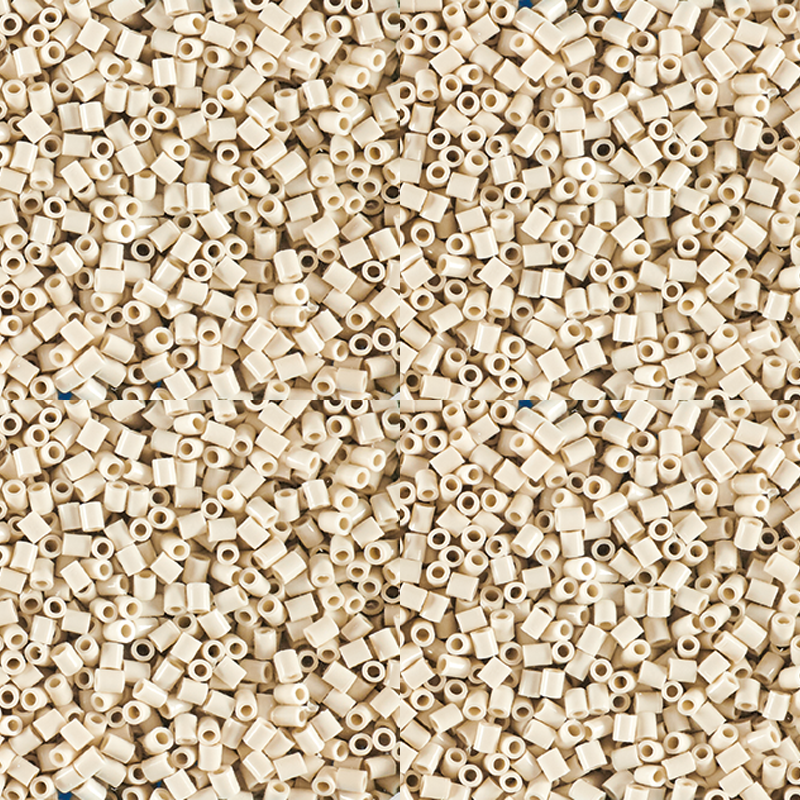
\includegraphics[width=6cm]{figs/cap5/hama.png}
	\end{center}
	\caption{Hama Beads$^{\ref{note:enlace81}}$} 
	\label{fig:hamabeads}
\end{figure}

\setcounter{footnote}{81} % Establecer la numeración de la siguiente nota al pie
\footnotetext[\value{footnote}]{\url{https://www.hamabeads.es/}\label{note:enlace81}}


Otro aspecto a tener en cuenta es que para la placa del módulo GPS es necesario soldarle unos pines (Figura \ref{fig:soldar}) para que posteriormente se pueda conectar los cables y evitar pérdida de señal. También es necesario agrandar con una taladradora los cuatro agujeros que tiene la antena del módulo para que puedan entrar bien los tornillos. 

\begin{figure} [h!]
	\begin{center}
		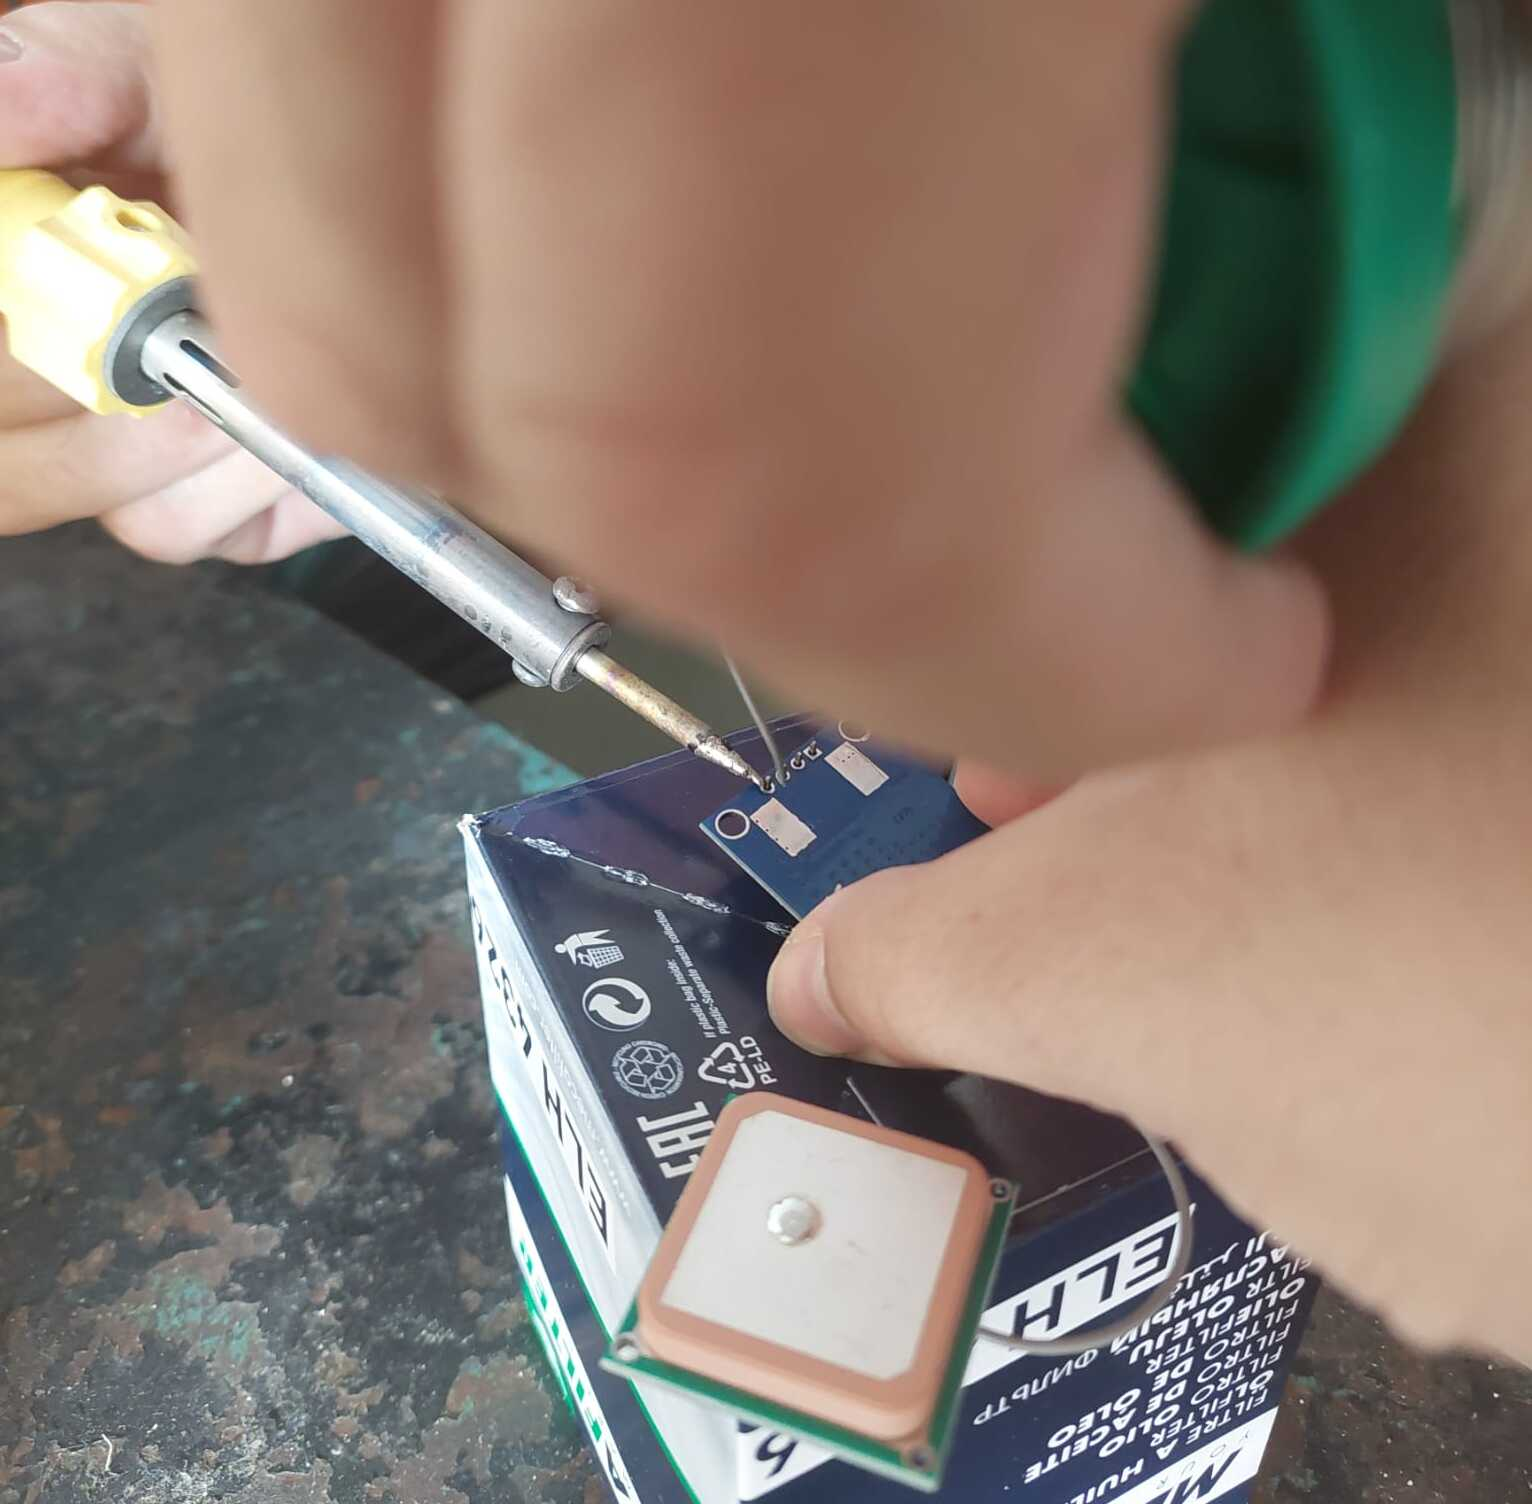
\includegraphics[width=8cm]{figs/cap5/soldar.jpeg}
	\end{center}
	\caption{Soldando pines al módulo GPS} 
	\label{fig:soldar}
\end{figure}

Una vez tenido en cuenta todos los aspectos anteriores, es necesario empezar a atornillar todas las piezas. Para facilitar el trabajo, el Cuadro \ref{cuadro:tornillos} muestra toda la tornillería necesaria. Además, las Figuras \ref{fig:pbasemontada}, \ref{fig:pcamaramontada}, \ref{fig:psuperiormontada} y \ref{fig:traseracon} han sido tomadas gracias a un diseño creado en FreeCAD\footnote{\url{https://github.com/RoboticsURJC/tfg-jlopez/blob/main/design/robotcompleto.FCStd}}, de Pibotj completo, que muestra el lugar donde se sitúa la tornillería del robot y ayudará al usuario facilitar el ensamblaje. La Figura \ref{fig:robotfreecad} muestra el robot completo montado. Los tornillos, tuercas y arandelas se han obtenido a través de Amazon\footnote{\url{https://www.amazon.es/410-tornillos-M2-avellanados-hexagonales/dp/B0C1BLSBLW/}}. Se recomienda usar un fijador para evitar que se aflojen los tornillos.

\begin{table}[H]
	\begin{center}
		\begin{tabular}{|c|c|c|c|c|}
			\hline
			Componente & Tornillos & Tuercas & Arandelas & Hama Beads blancas\\
			\hline
			Motores & 12 M2 10mm & 12 & 24 &\\
			\hline
			Picamera (base) & 2 M2 10mm & 2 & 4 &\\
			\hline
			Picamera (cámara) & 2 M2 12mm & 2 & 12 &\\
			\hline
			Raspberry Pi & 4 M2 12mm & 4 & & 4\\
			\hline
			Placa GPS & 4 M2 16mm & 4 & 8 & 4\\
			\hline
			Antena GPS & 4 M2 16mm & 4 & & 4\\
			\hline
			Sujección entre placas & 4 M2 16mm & 4 & 8 &\\
			\hline
			Sujección trasera & 1 M2 16mm & 1 & 2 &\\
			\hline
		\end{tabular}
		\caption{Tornillería necesaria}
		\label{cuadro:tornillos}
	\end{center}
\end{table}

\begin{figure} [h!]
	\begin{center}
		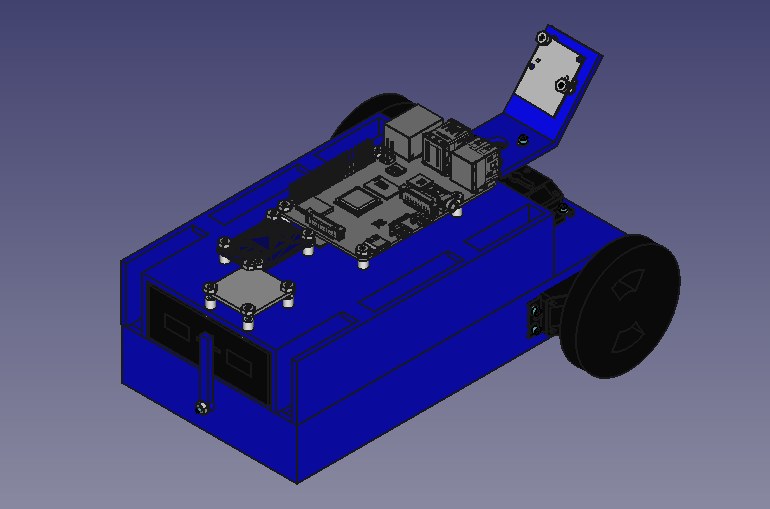
\includegraphics[width=12cm]{figs/cap5/completo3.png}
	\end{center}
	\caption{Robot completo montado en FreeCAD} 
	\label{fig:robotfreecad}
\end{figure}


Para sujetar el cable de alimentación de la Raspberry Pi, se ha utilizado una brida. Para optimizar el espacio ocupado por los cables, se han empleado gomas pequeñas. Además, se están utilizando diez cables macho-hembra para alimentar los dos motores y el módulo GPS, mientras que el motor de la cámara ha quedado sin conectar.

En la realización de este proyecto se han probado dos tipos de ruedas: las del kit ActivityBot y las de goma azul. Según la aplicación, se puede optar por una u otra. A continuación, se explicará el montaje de cada tipo.

Para utilizar las ruedas del kit ActivityBot, simplemente es necesario atornillarlas al robot con el tornillo que viene incluido, ya que estas ruedas están diseñadas específicamente para motores Parallax. El robot tendría el aspecto que se muestra en la Figura \ref{fig:ab}.

\begin{figure} [h!]
	\begin{center}
		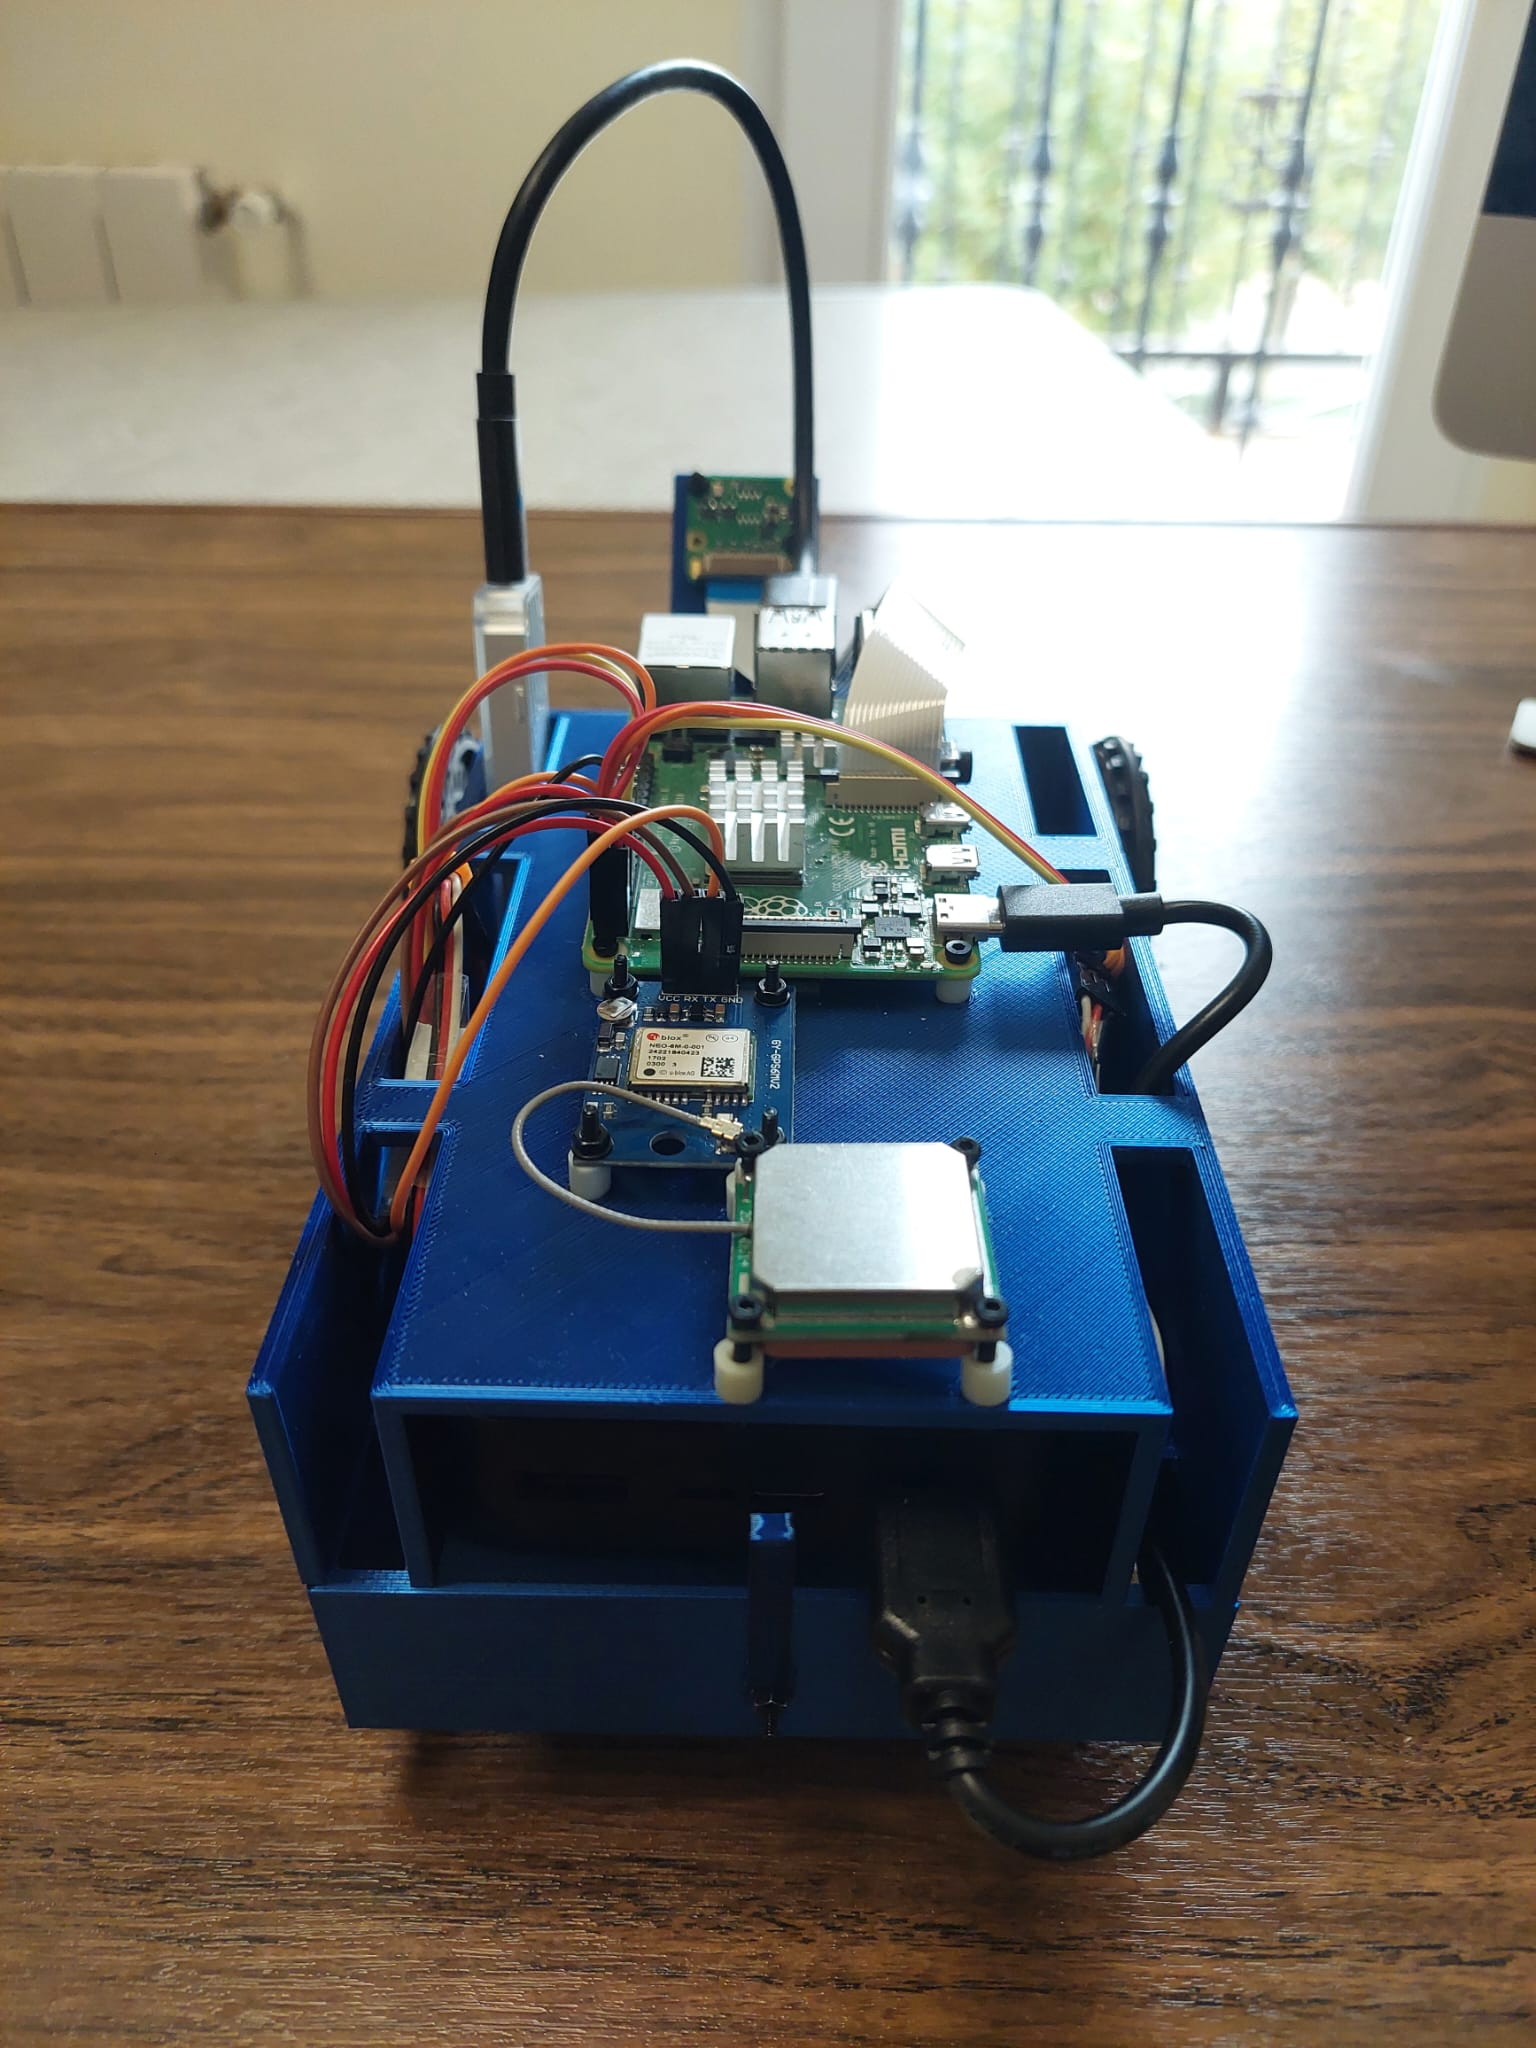
\includegraphics[width=12cm]{figs/cap5/ab.jpeg}
	\end{center}
	\caption{Pibotj con ruedas de ActivityBot} 
	\label{fig:ab}
\end{figure}

Por otro lado, si se prefieren ruedas como las de goma azul, se requerirán algunas modificaciones. En primer lugar, se deberá usar una sierra para cortar las partes sobrantes (Figura \ref{fig:rae}, izquierda). También será necesario perforar la rueda con un taladro para que el tornillo que conecta al motor encaje fácilmente. Luego, se deben colocar dos topes de motor sobre la superficie lisa de la rueda (Figura \ref{fig:rae}, derecha) y hacer los agujeros correspondientes para atornillarlos. En este caso, se han utilizado siete tornillos M2 de 8 mm. El robot con estas ruedas tendría el aspecto que se muestra en la Figura \ref{fig:ra}.

\begin{figure}[ht!]
	\centering
	\begin{minipage}{0.45\linewidth}
		\centering
		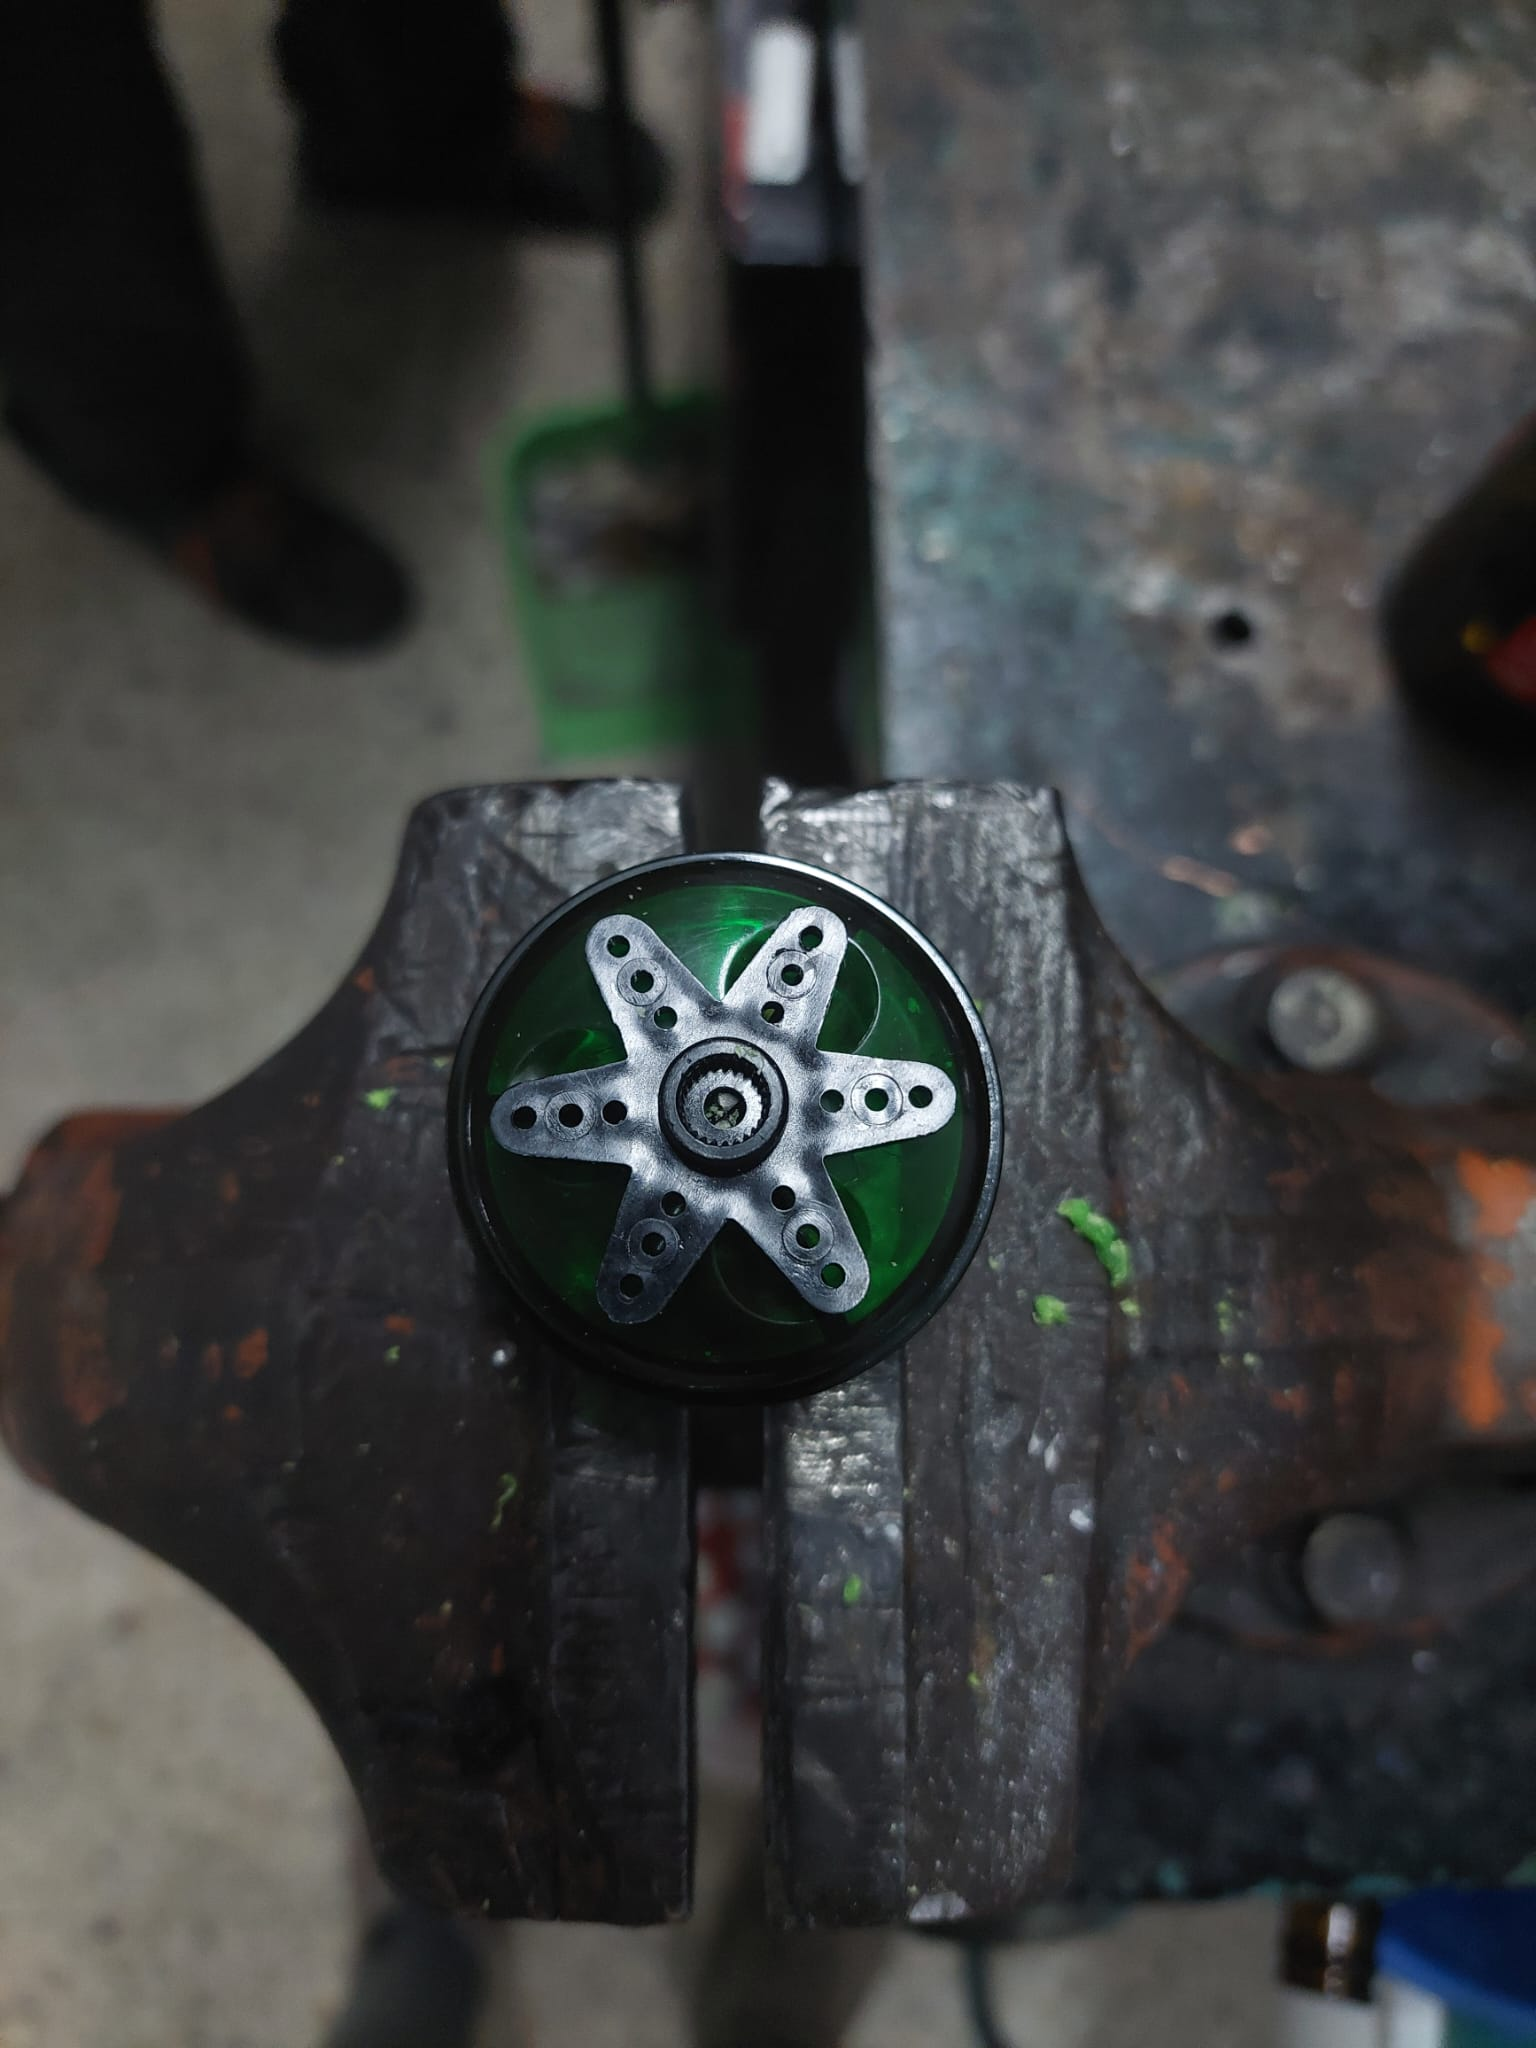
\includegraphics[width=\linewidth]{figs/cap5/creacionra1.jpeg}
		\caption*{\centering}
	\end{minipage}
	\hspace{1cm}
	\begin{minipage}{0.45\linewidth}
		\centering
		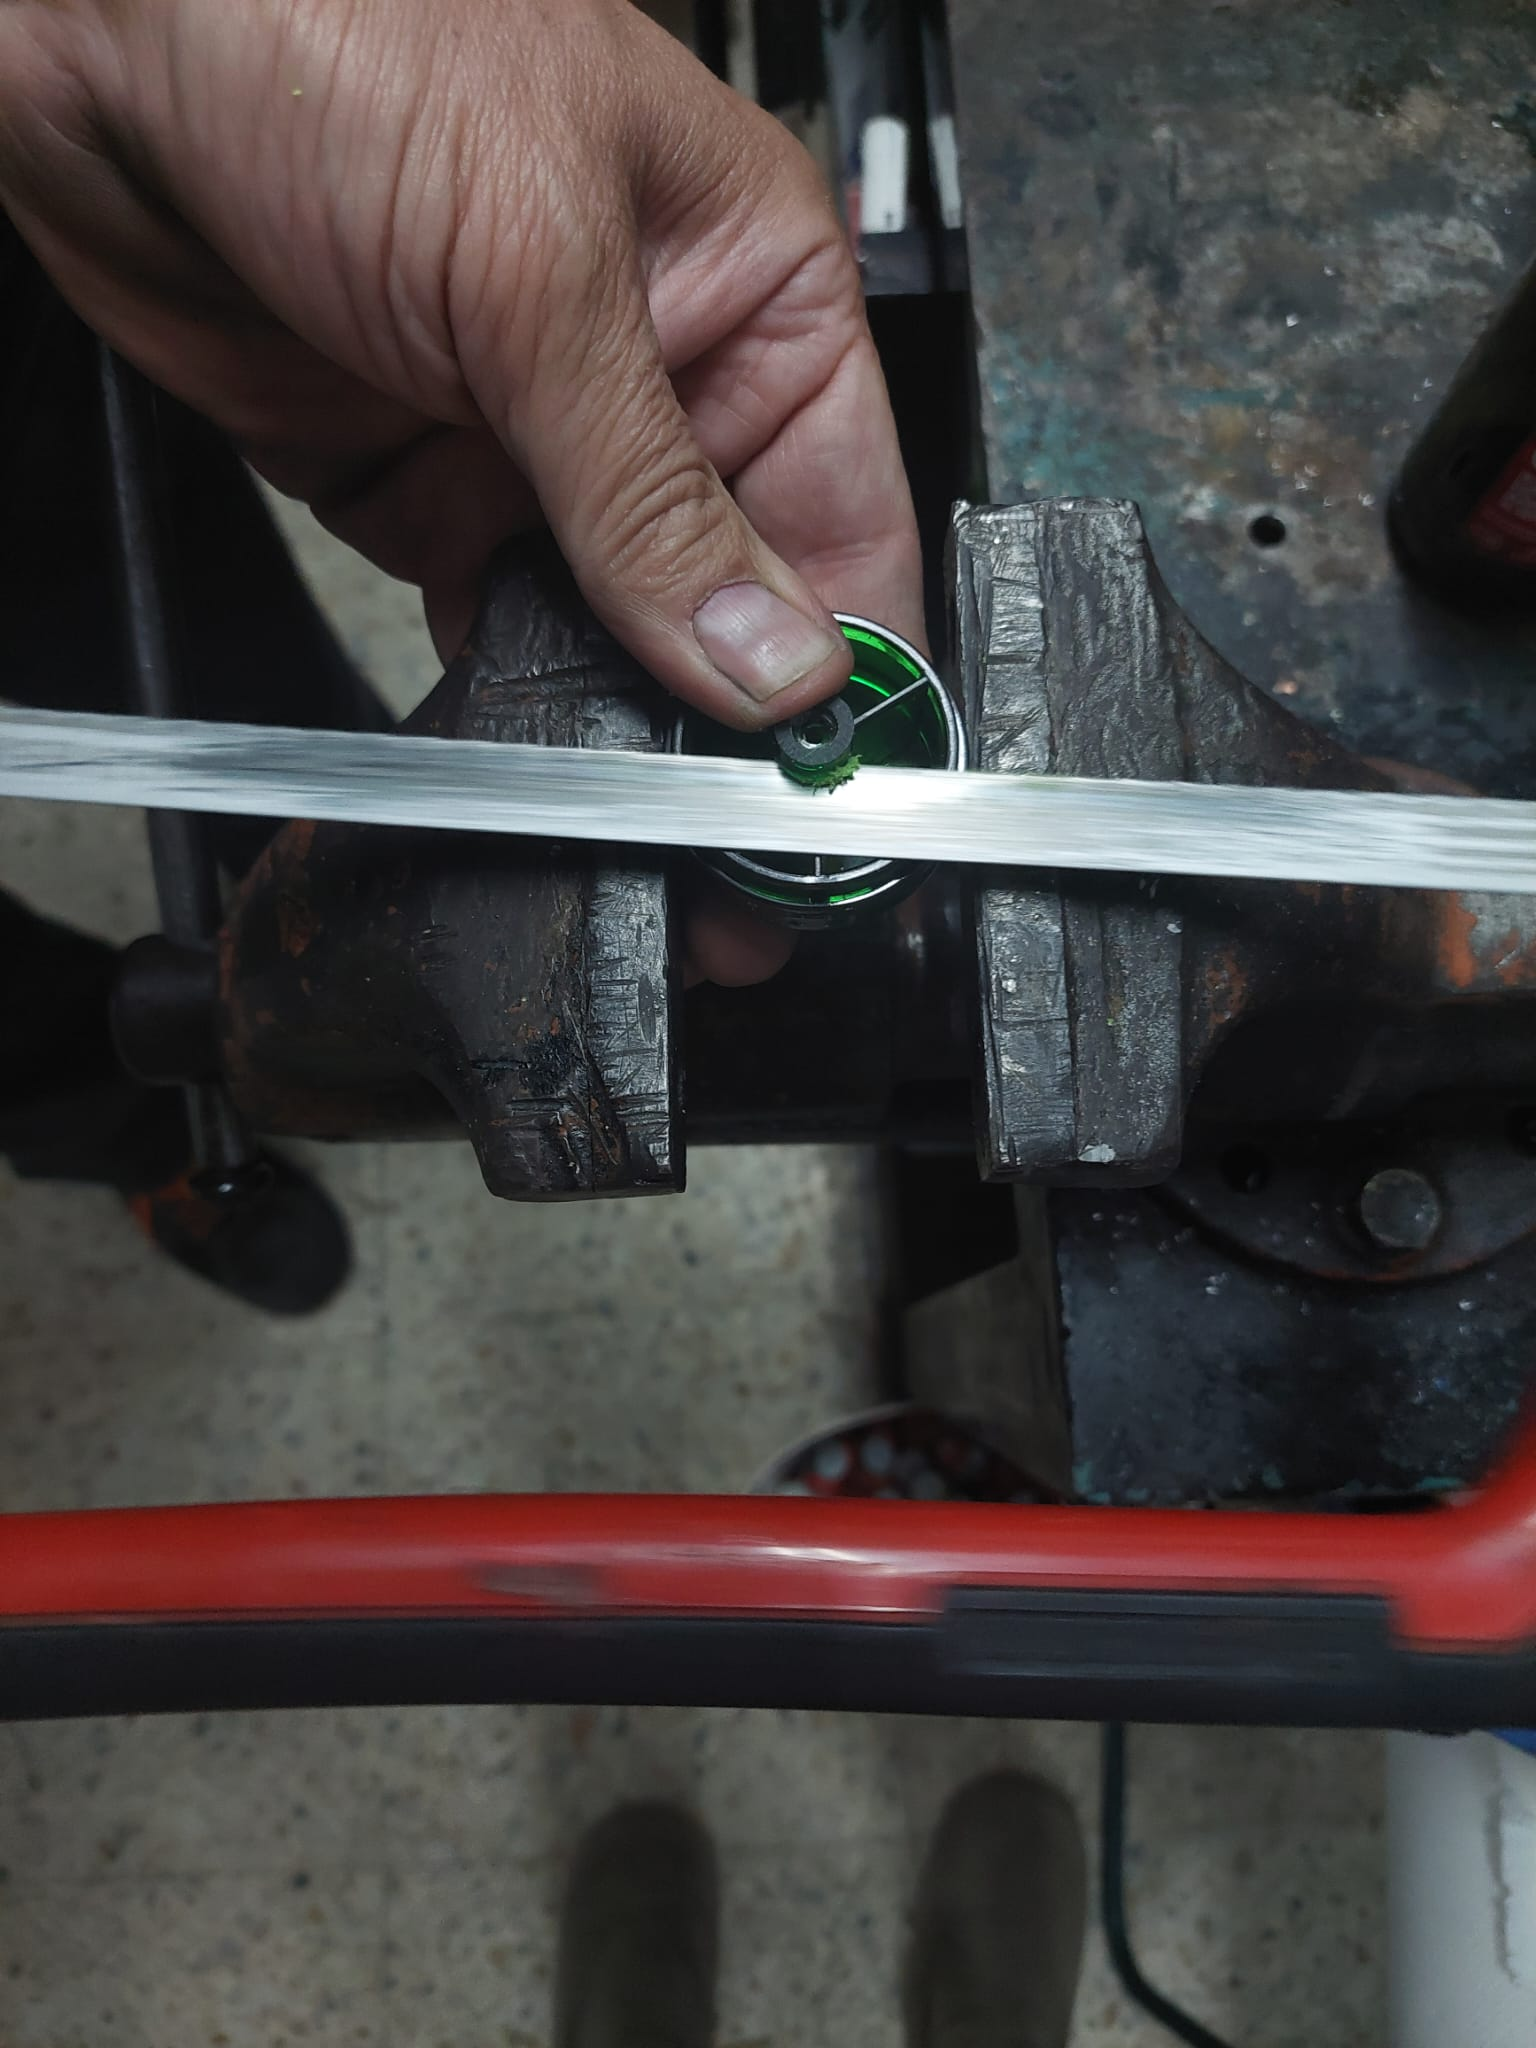
\includegraphics[width=\linewidth]{figs/cap5/creacionra2.jpeg}
		\caption*{\centering}
	\end{minipage}
	\caption{Ensamblaje ruedas azules}
	\label{fig:rae}
\end{figure}


\begin{figure} [h!]
	\begin{center}
		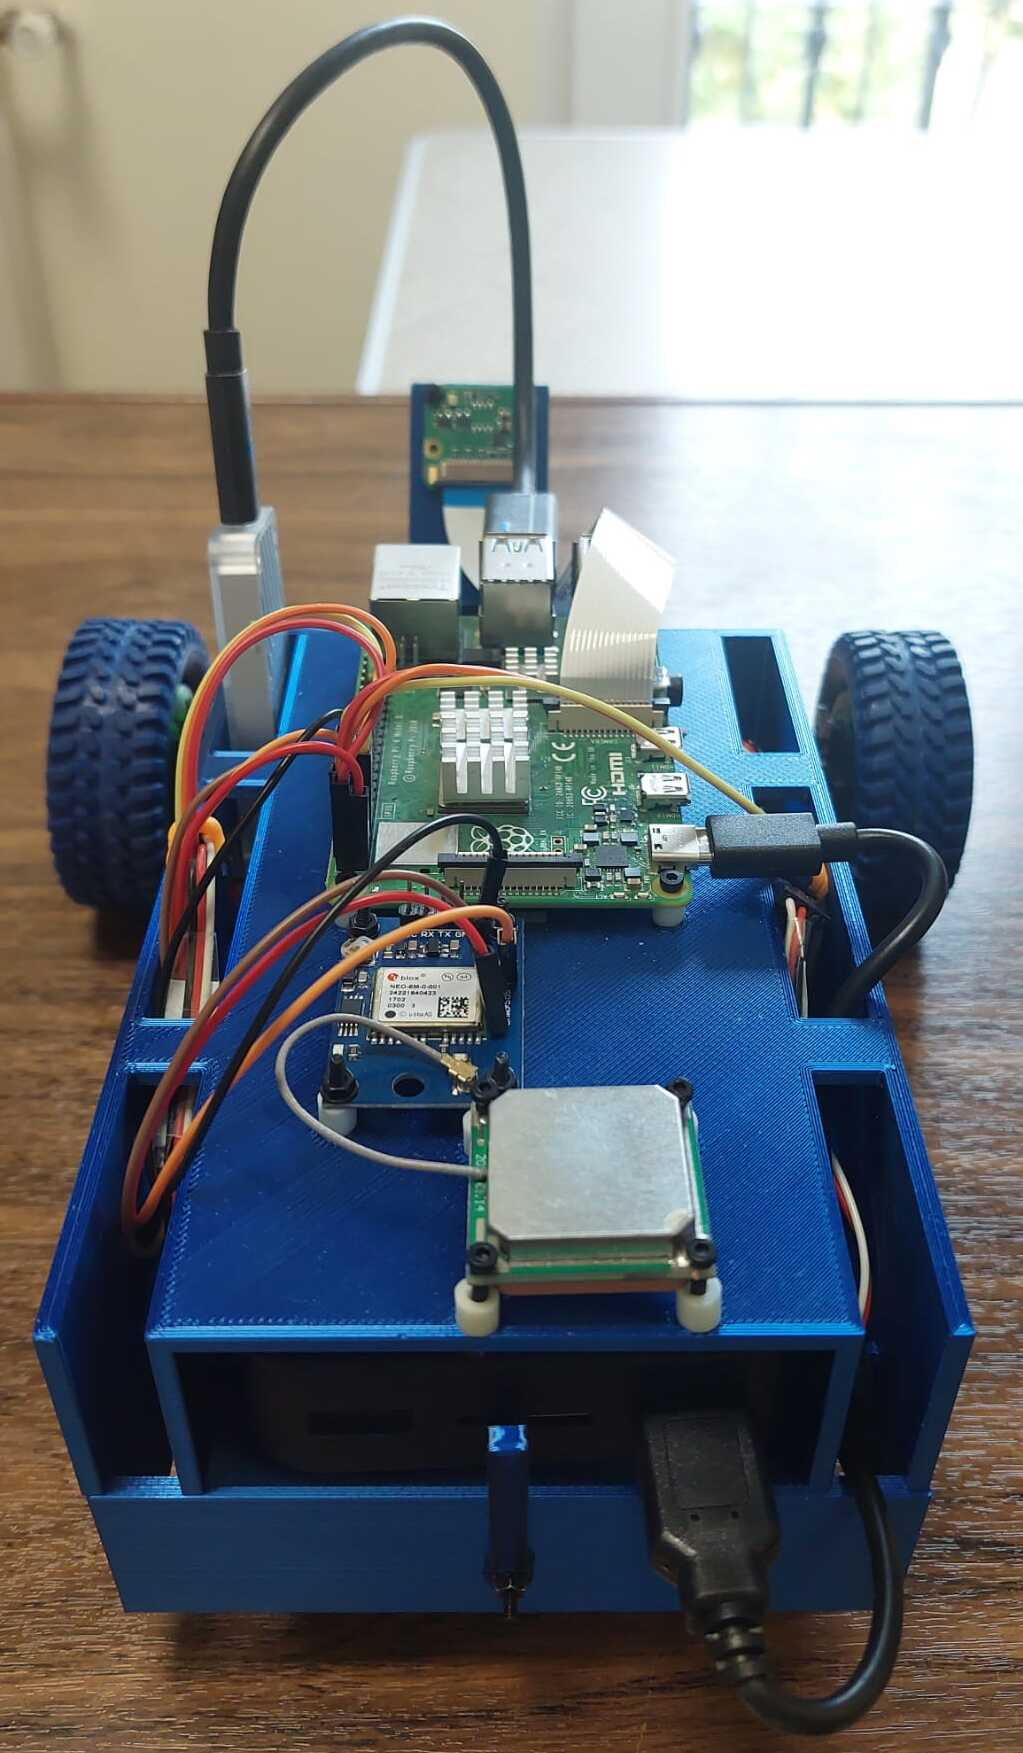
\includegraphics[width=12cm]{figs/cap5/ra.jpeg}
	\end{center}
	\caption{Pibotj con ruedas azules} 
	\label{fig:ra}
\end{figure}


Para resumir lo explicado, el Cuadro \ref{cuadro:costetotal} enumera todos los componentes necesarios para construir a Pibotj, junto con sus precios respectivos.

\begin{table}[H]
	\begin{center}
		\begin{tabular}{|c|c|}
			\hline
			Componente & Precio \\
			\hline
			Motores Parallax & 34€ \\
			\hline
			Picamera &  18€ \\
			\hline
			Raspberry Pi & 65€ \\
			\hline
			Módulo GPS & 9€ \\
			\hline
			Ruedas ActivityBot/Azules & 9€ \\
			\hline
			Google Coral USB & 65€ \\
			\hline
			Powerbank & 30€ \\
			\hline
			Rueda Loca & 1,13€ \\
			\hline
			Tornillos, tuercas, arandelas y Hama Beads & 3€ \\
			\hline
			Cables, gomas y brida & 3€ \\
			\hline
			Rollo de PLA gastado & 10€ \\
			\hline
		\end{tabular}
		\caption{Coste proyecto}
		\label{cuadro:costetotal}
	\end{center}
\end{table}

El coste total del proyecto es de 247,13€ por lo que demuestra que está por debajo del límite establecido de 250€ y cumple con el objetivo establecido del Capítulo 3.\\\\\\\\\\


Una vez alcanzado este punto, se ha completado el desarrollo del hardware necesario para la construcción de Pibotj. A continuación, se procederá a dar vida a este hardware para alcanzar el objetivo del proyecto, lo cual se detallará en el siguiente capítulo.

